%%%%%%%%%%%%%%%%%%%%%%%%%%%%%%%%%%%%%%%%%%%%%%%%
% BOZZA PER TESI DI LAUREA IN LATEX
%%%%%%%%%%%%%%%%%%%%%%%%%%%%%%%%%%%%%%%%%%%%%%%%

%\documentclass[12pt,titlepage]{book}
\documentclass[a4paper,twoside,12pt]{article}
\usepackage[british]{babel}
\usepackage{gensymb}
\usepackage[toc,page]{appendix}
%\usepackage{graphics}
%\usepackage{url,amsfonts,epsfig}
%\usepackage[applemac]{inputenc} %comando per le lettere accentate se usate mac  
\usepackage[utf8]{inputenc} % comando per le lettere accentate se usate pc  
\usepackage[nottoc]{tocbibind}
\usepackage{unipitesi}
\usepackage[font=small]{caption}
\usepackage{subcaption}
\usepackage{tabu}
\usepackage{hyperref}
\usepackage{textcomp}
\usepackage{multirow}
\usepackage{graphicx}
\usepackage{amsmath}
\usepackage{amssymb}
\usepackage{xcolor}
\usepackage{verbatim}
\graphicspath{ {Images/} }

\hypersetup{
colorlinks=true,
linkcolor=blue,
urlcolor=blue
}
\urlstyle{same}

\pagestyle{headings}

\definecolor{dred}{RGB}{200,0,0}
\definecolor{dblue}{RGB}{0,0,200}

%\title{\textsc{Analysis of performance of ATLAS experiment Phase 2 inner tracker}}
%\author{Federico Massa}

\begin{document}

%%%% Opzione per interlinea 2
%%%\baselineskip 18pt

%\maketitle

\titolo{\textit{Tracking performances of the ATLAS detector} \\
			\textit{and impact on the $H\rightarrow ZZ^{*}\rightarrow 4\mu$ channel}}
\laureando{Federico Massa} 
\corsodilaureamagistrale{Fisica} 
\relatore[Prof.]{Giorgio Chiarelli} 
\secondorelatore[Dott.]{Claudia Gemme} 
%\controrelatore[Prof.]{prof3} 
\annoaccademico{2015-2016} 
\data{data}
\maketitle


\tableofcontents
%%\listoffigures
%%\listoftables
\newpage

\begin{comment}
\begin{abstract}
La fase di High Luminosity LHC offrirà nuove opportunità per esplorare eventi estremamente rari, ed in particolare per studiare la fisica e le proprietà del bosone di Higgs.
L’esperimento ATLAS, per sfruttare al massimo questa possibilità, sostituirà l’Inner Tracker  all’attuale Inner Detector.
A causa dell'elevato numero di eventi di pileup ($>200$) previsti, il tempo richiesto dalla simulazione Monte Carlo risulta proibitivo. E’ stato, pertanto, sviluppato un metodo ad-hoc che permette di simulare solo le regioni di interesse in modo accurato, confrontando differenti configurazioni del rivelatore. In questo studio presentero' i risultati ottenuti relativamente al canale\\ {$H\rightarrow ZZ^*\rightarrow 4\mu$}
\end{abstract}
\end{comment}

\newpage

\section*{Introduction} \label{sec:introduction}
This thesis is centered on the expected performance of the tracking system (ITk) which is being designed for the ATLAS upgrade and that will replace the
current Inner Detector in the High Luminosity LHC phase (HL-LHC), scheduled to start in 2026. \\

The Large Hadron Collider (LHC) accelerator worked at a center-of-mass energy of 7 TeV during Run-1 and 13 TeV during Run-2. It is scheduled to be upgraded in two different stages: the first one will begin after the end of Run 2 during the Long shutdown 2 (LS2) in 2019-2020, when LHC will reach its maximum design energy of 14 TeV; the second one will start at the end of Run 3 during the Long shutdown 3 (LS3) in 2024-2026 (Fig.\ref{fig:HLLHC_Plan}). The latter upgrade stage will lead to what is known as High-Luminosity LHC (HL-LHC) during which the
luminosity will reach the maximum value of $7.5 \times 10^{34}\ cm^{-2}s^{-1}$, corresponding to approximately $3000\ fb^{-1}$ during ten years of data taking. \\

\begin{figure} [h]
	\includegraphics[width=\textwidth]{HLLHC_Plan}
	\caption{LHC/HL-LHC Plan as scheduled in 2015\cite{scoping}.}
	\label{fig:HLLHC_Plan}
\end{figure}

HL-LHC will allow to study new physics processes, such as extra dimensions or the ones predicted by SUSY models, as well as improve Standard Model measurements. In particular, Higgs boson 
couplings are expected to be measured with a precision between 5\% and 30\%\cite{loi}. Thanks to the increased luminosity, it will be possible to observe the Higgs boson in extremely
rare channels, which are impossible to measure at LHC.\\

By the end of Run 3, ATLAS detector will be using 15-20 years old components. In particular,
the highly irradiated Inner Detector pixels and strips will have reached the end of their
lifetime and the transition radiation tracker will reach 100\% occupancy at that luminosity. Thus, the Inner Detector must be completely substituted by the Inner Tracker (ITk), which will
have to guarantee the same or an improved performance in the harsh conditions of HL-LHC while maximizing the acceptance. At design luminosity, the expected number of in-time pileup events will be $<\mu > = 200$, a much
higher value than the one expected at the end of Run 3 ($<\mu > = 80$) and even more if 
compared to the current one ($<\mu > = 23$), introducing new challenges in the pattern
recognition. The increase of the number
of collisions per bunch crossing leads to new requirements on the front-end electronics, trigger and data acquisition system that cannot be met by the current apparatus, thus leading to a 
substantial upgrade of the electronics. Moreover, the Reference Scenario of the Scoping Document\cite{scoping} proposes an increase of the geometrical acceptance of the detector by extending the $|\eta|$ coverage to $4.0$, which requires either the substitution (such as in the case of ITk) or the addition of new detectors (muon chambers,
calorimeter system). \\

Other than detector and hardware upgrades, HL-LHC will require software upgrades to meet the needs of the new detectors, handle large event samples and adapt to multi-processor
architectures. To deal with the simulation size and time requirements it will be necessary to mix fast simulation techniques (using detector parametrisations) with full simulation at event level.\\

Here we present a fast simulation method that allows to simulate the effect of the high number of pile-up events on the tracking and physics performances, applied to single pion and $H \rightarrow ZZ^{*} \rightarrow 4\mu$ Monte Carlo samples. 

\clearpage

\section{ATLAS Detector} \label{sec:detector}

\begin{figure} [h]
	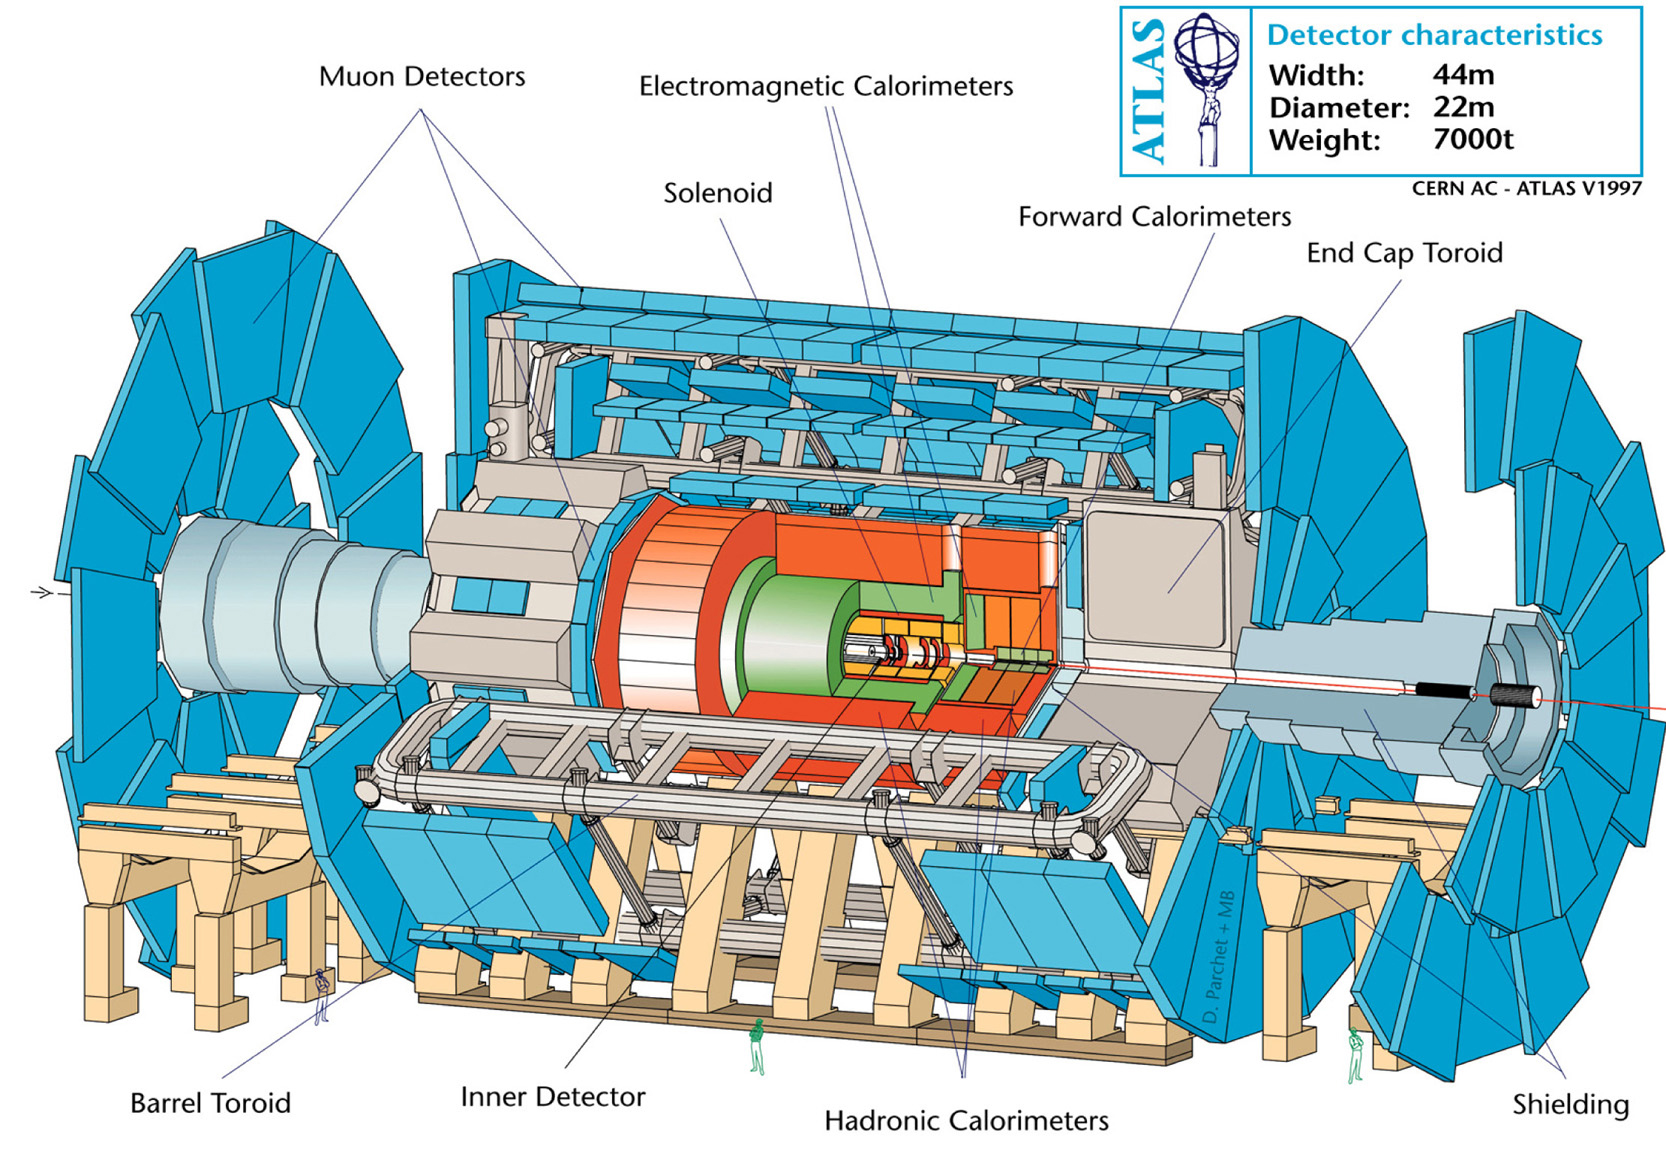
\includegraphics[width=\textwidth]{atlasdet}
	\caption{Current ATLAS detector.}
	\label{fig:current_atlasdet}
\end{figure}

This section briefly describes the current experimental apparatus, shown in Figure \ref{fig:current_atlasdet}, and the reasons as to why it cannot withstand the conditions of HL-LHC. The ATLAS detector is is a magnetic spectrometer, therefore its components are:
\begin{itemize}
\item the \textbf{magnet system};
\item the \textbf{inner detector};
\item the \textbf{electromagnetic calorimeter};
\item the \textbf{hadronic calorimeter};
\item the \textbf{muon spectrometer};
\item the\textbf{trigger system};
\item the\textbf{data acquisition system (DAQ)}.
\end{itemize}

In the following sections these elements are briefly described, outlining the main upgrades that will be applied for the high luminosity phase. 

\subsection{The magnet system}\label{sec:magnet}

\begin{figure} [h]
	\centering
	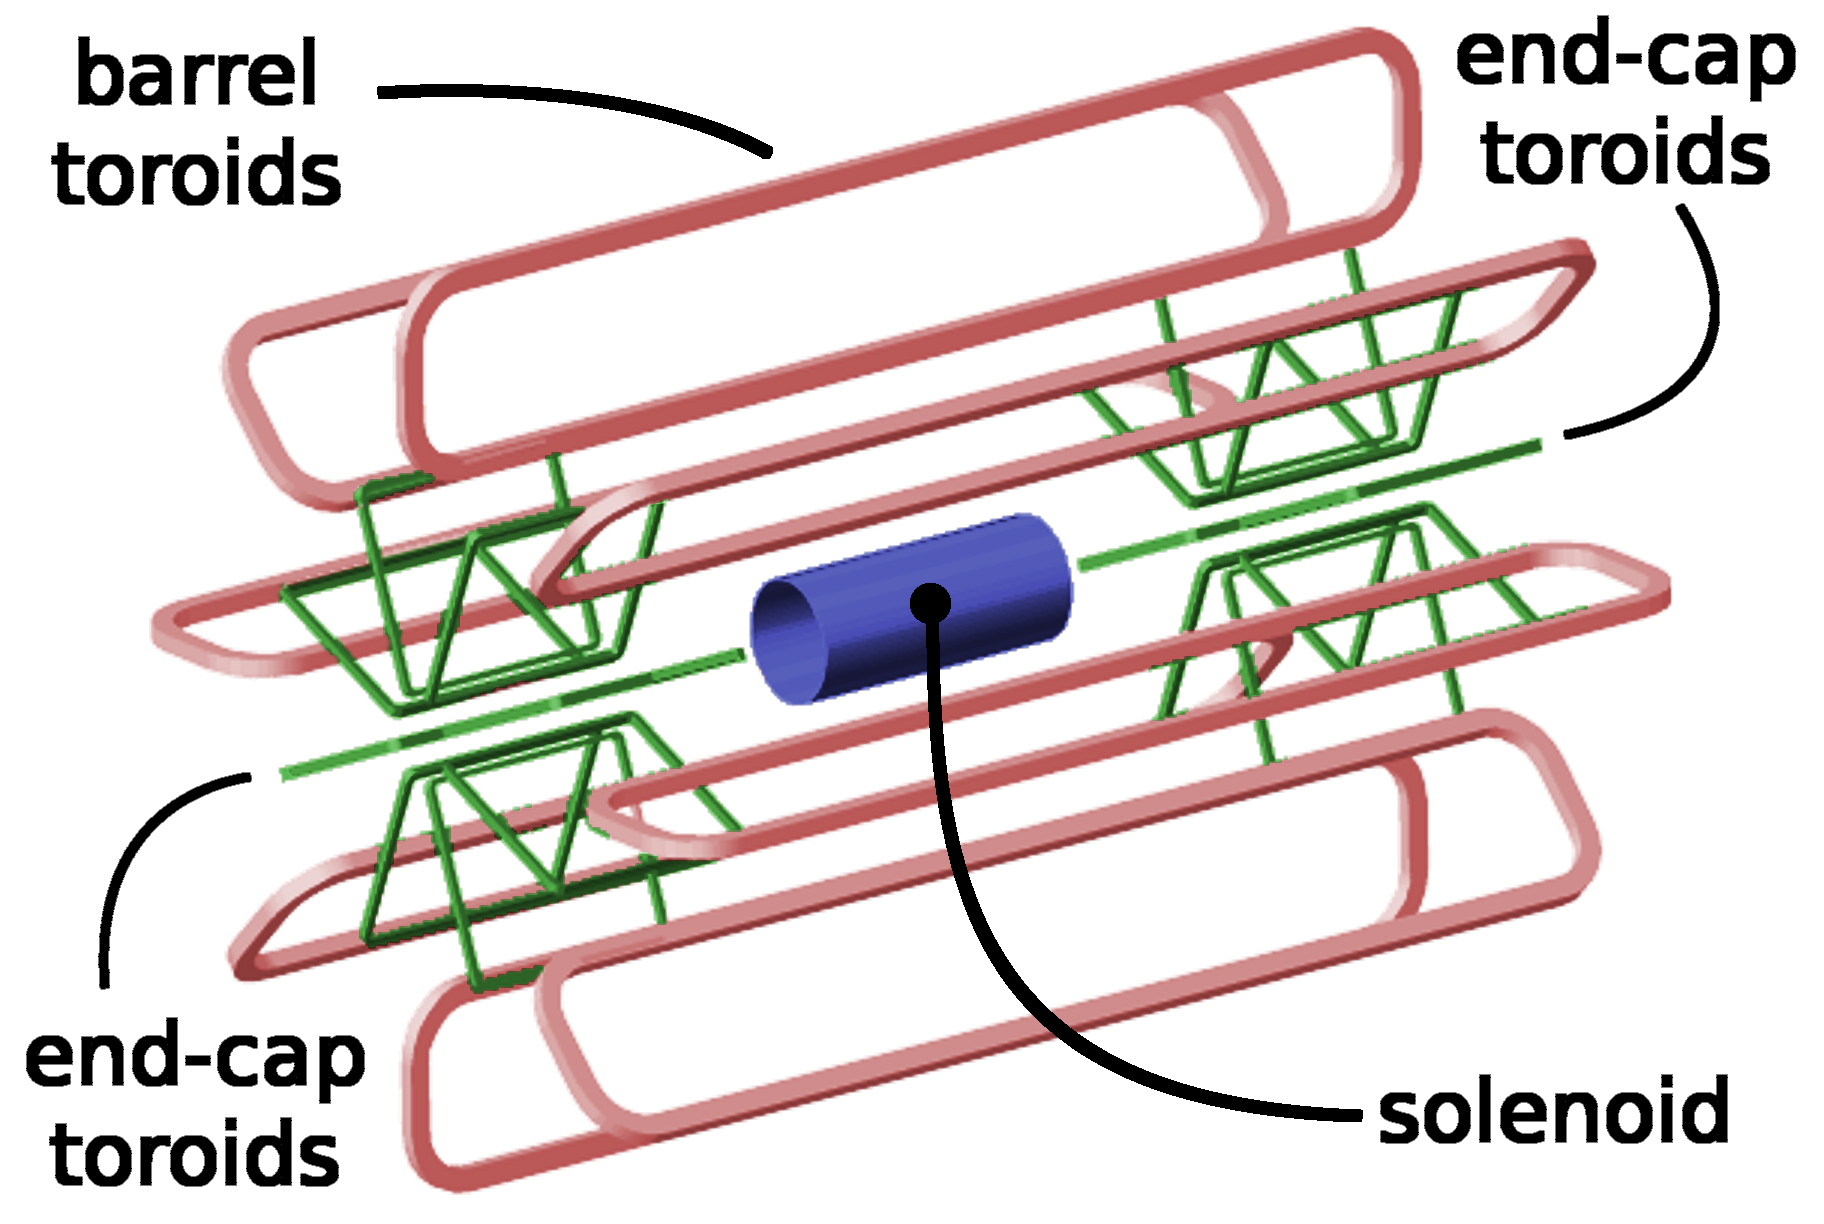
\includegraphics[scale=0.13]{magnetSystems}
	\caption{ATLAS magnet system\cite{magnet_system_picture}.}
	\label{fig:magnet_system_picture}
\end{figure}

The current magnet system (Fig.\ref{fig:magnet_system_picture}) comprises four superconducting magnets\cite{magnet_system}, for charged particles bending and momentum measurement in the $8000\ m^3$ volume of the apparatus.\\

The \textit{Central Solenoid Magnet} encloses the tracking volume and provides a $2\ T$ magnetic field along the beam axis and minimal thickness in order to reduce the degradation of photon and electron energy resolution in the subsequent calorimeter layers.\\

The \textit{Barrel} and \textit{Endcap Toroids} provide a tangential magnetic field of about $1\ T$ for the muon detectors, both in the radial and the forward region.\\

As the current magnet system already matches HL-LHC needs, it will not require an
upgrade.

\subsection{The Inner Detector}\label{sec:detector:tracker}

\begin{figure} [h]
\centering
	\includegraphics[width=.75\textwidth, angle=-90]{NewID}
	\caption{ATLAS Inner Detector layout\cite{Aad:2008zzm}.}
	\label{fig:IDLayout}
\end{figure}

The ATLAS \textbf{Inner Detector} (ID), whose current layout is shown if Fig.\ref{fig:IDLayout}, is designed to measure the momentum of the
charged particles tracks with $p_{T}$ greater than $\simeq$ $500\ MeV$ and 
within $|\eta| < 2.5$, with the capability to reconstruct multiple primary vertices, as well as vertices displaced from the primary\cite{Aad:2008zzm}. \\

The ID is contained in a cylindrical envelope (with the axis along the z-axis) that extends
$\pm\ 3512\ mm$ in length and $1150\ mm$ in radius. The whole system is placed inside
the central solenoid magnet. The ID is consists of three sub-detectors: the innermost section provides
high resolution pattern recognition and secondary vertexing capability using \textit{silicon pixel layers}, the middle one consists of stereo pairs of \textit{silicon microstrip} (SCT) layers and the outermost one consists of the \textit{Transition Radiation Tracker} (TRT). During 2014 ATLAS upgrade, the \textit{Insertable B-Layer} (IBL), a fourth pixel barrel layer, was added to avoid the decrease of performances after the luminosity upgrade of LS1. \\

Each one of these detectors is subdivided into a \textit{barrel} ($|\eta \lesssim 1.0$) region, in which the sensor modules 
are organized tangentially with respect to a circle around the beam axis and an \textit{end-cap} region, in which they are placed perpendicularly with respect to the beam axis, producing
a disk resemblant shape.\\

The \textit{pixel} barrel layout consists of 3 layers placed at approximate radii $50.5$, $88.5$ and $122.5\ mm$ with respect to the beam 
axis. The IBL was added during the LS1 as the
innermost pixel layer at radius $33.5\ mm$. In the end-cap region, three disks per side were chosen,
at z position respectively $495\ mm$, $580\ mm$, $650\ mm$. \\

The \textit{SCT} barrel layout consists of four layers at radii $300\ mm$, $373\ mm$, $447\ mm$ and $520\ mm$. The end-cap region is instead composed by 9 disks per side with variable
inner radii and z-position ranging from $850\ mm$ to $2720\ mm$. \\

The \textit{TRT} barrel layout is formed by straws parallel to the beam axis at radii from $563\ mm$ to $1066\ mm$,
while the end-cap region consists of radially wound straws with z ranging from $850\ mm$ to 
$2710\ mm$. This detector can track particles up to $|\eta| < 2.0$.

\subsubsection*{Pixel and SCT}

The pixel and SCT sensors are designed to maintain their performance during the detector
lifetime at nominal luminosity\cite{Aad:2008zzm}. As the integrated radiation dose has significant consequences
on these sensors, they are operated at a temperature between $-10\ ^{\circ}C$ and $-5\ ^{\circ}C$.\\

\textit{Pixel sensors} of the Run 1 ID (thus excluding IBL) are $250\ \mu m$ thick detectors which are mounted on oxygenated n-type wafers, with the pixel on the $n^+$ side. About 90\% of the pixel on a sensor have a nominal 
size of $50 \times 400\ \mu m^2$, while the rest are $50 \times 600\ \mu m^2$ large and are placed
at the front-end chips on a module. There are a total of 1744 identical pixel sensors with an external dimension of $19 \times 63\ mm^2$, each composed by 47232 pixels. For reasons of space, there are four ganged pixels on each column of the front-end chip, thus resulting in a total of 46080 readout channels. \textit{IBL pixels} are, instead, $50 \times 250\ \mu m^2$ large to 
ensure a highly precise measurement of the coordinates near the interaction point\cite{IBL}. Two 
different technologies have been implemented in the central and forward IBL region, which
results in a different sensor thickness and module sizes.\\

The \textit{SCT} consists of a total of 15912 silicon strips sensors with thickness $285 \mu m$. Each sensor consists of 768 strips of $12\ cm$ length, with average pitch of $80\ \mu m$.
On each SCT module there are two back-to-back sensors with a relative angle of $40\ mrad$,
which allows the extraction of a second coordinate. The readout electronis is placed at the end of each sensor.\\

Pixel and SCT system will be completely replaced for HL-LHC, as described in sec.\ref{sec:tracking}.

\subsubsection*{TRT}
The basic elements of \textit{TRT} consist of $4\ mm$ diameter tubes\cite{Aad:2008zzm}. For both the barrel
and end-cap sections, the anodes are made of $31\ \mu m$ diameter, $\pm\ 71.2\ cm$ 
active length tungsten wires 
connected to the front-end electronics and grounded. The wires are carefully aligned within
the straw, with a maximum tolerance of $300\ \mu m$. The barrel section contains about 
50000 straw tubes, whereas the end-cap contains approximatively 320000,
for a total of 420000 electronic channels\cite{ATLAS:1997ag}. This detector typically provides
an almost continuous tracking of the particles traversing it, with an average of 36 measurements per track.\\

Due to the strict requirement of HL-LHC, the TRT will be removed, and its space will be allocated for the new
Inner Tracker (ITk), which is the main focus of this thesis and will be described in detail in sec.\ref{sec:tracking}.

\subsection{Calorimeter system}

The ATLAS experiment  relies on an electromagnetic and a hadronic calorimeter to identify and measures energies and direction of photons, electrons, hadrons, jets and neutrinos. 
Both compartments are divided into a central and a forward region (Fig.\ref{fig:current_Cals}). The electromagnetic calorimeters are based on the liquid Argon technology,
whereas the hadron calorimeters are either liquid Argon (forward region) or tile calorimeter (central).\\

\begin{figure} [h]
	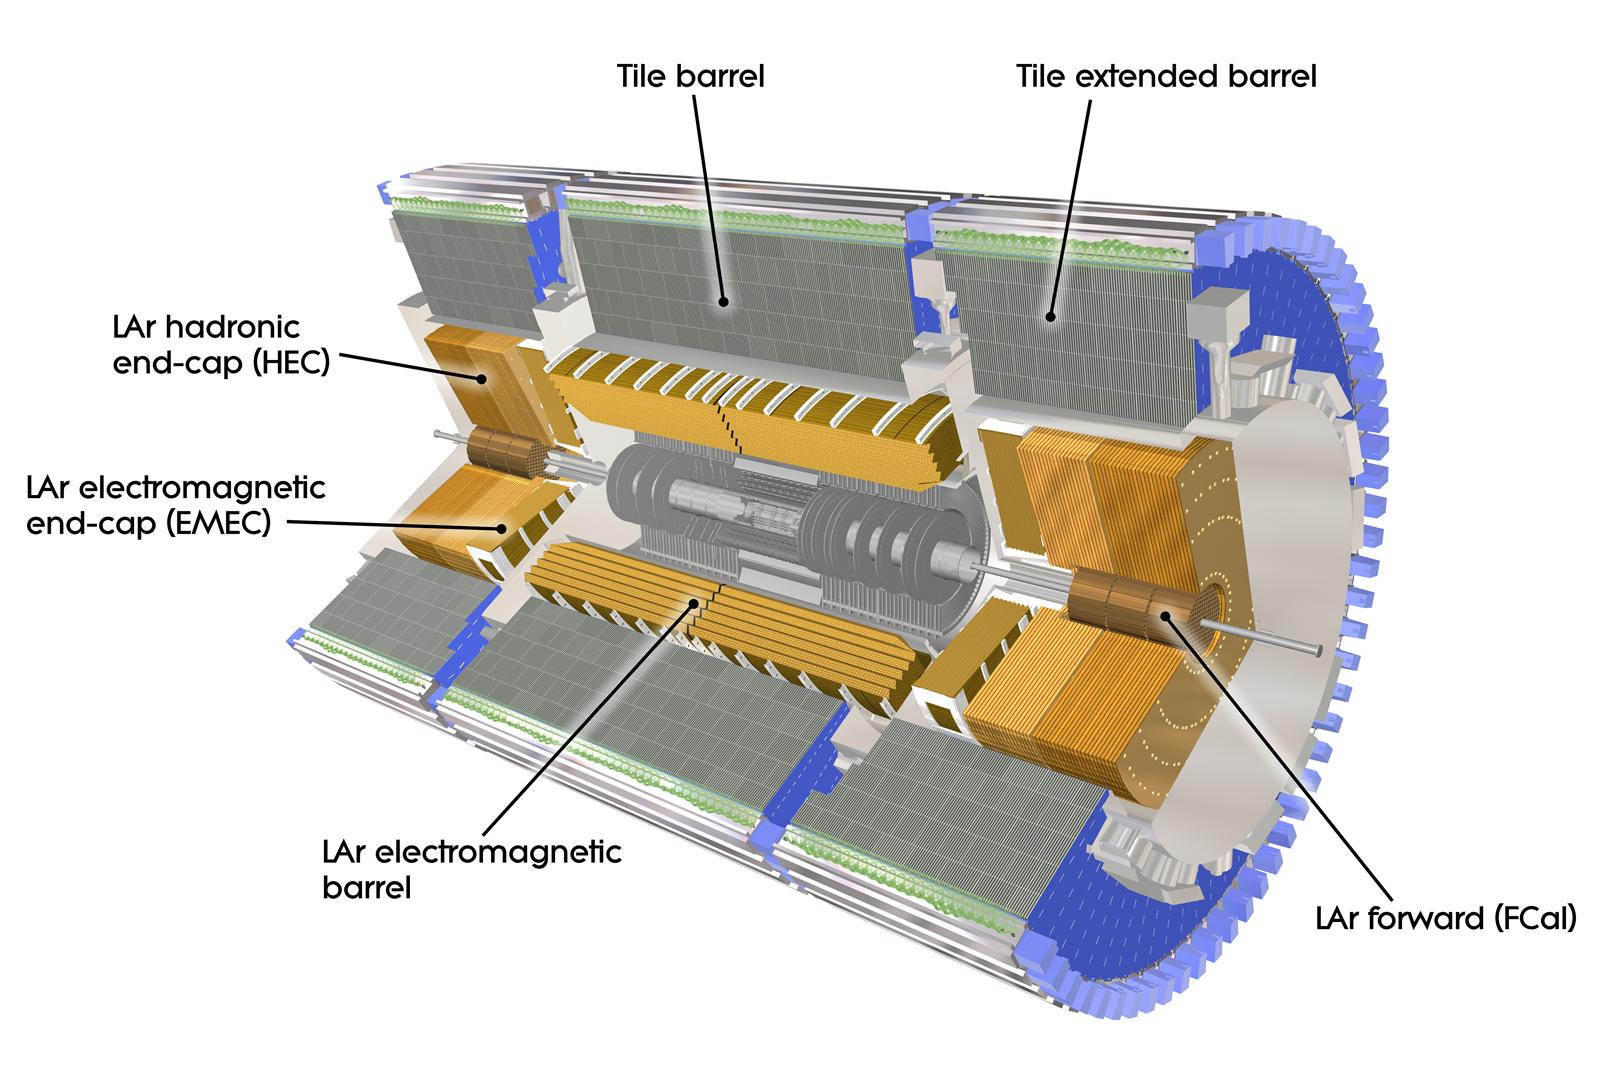
\includegraphics[width=\textwidth]{current_Cals}
	\caption{ATLAS Calorimeter System.}
	\label{fig:current_Cals}
\end{figure}

\subsubsection*{Liquid Argon Calorimeters}\label{sec:LAr}
Several components of the ATLAS calorimeter use liquid Argon (LAr) as active medium\cite{current_EMCal}. The electromagnetic barrel and endcap (EMEC) are entirely built this way, but also the Hadronic Endcap Calorimeter (HEC) and the Forward Calorimeter (FCal). \\[2pt]
The \textbf{electromagnetic calorimeter} uses lead as absorber and is designed to trigger on and to provide precision measurements of electrons, photons, jets, and missing $E_T$ .
The full cryostat of the \textit{barrel section} is $6.8\ m$ long, with the inner and outer radius being respectively $1.15\ m$ and $2.25\ m$ and ranges in $|\eta|$ from 0 to 1.7.  The \textit{endcap section} consists of two concentric wheels, the larger one ranging in $|\eta|$ from 1.4 to 2.5, the smaller from 2.5 to 3.2. In addition, a \textit{presampler} layer was inserted behind the cryostat wall to correct for the losses in the upstream material. 
%The amount of inactive material due to the solenoid
%accounts for $0.63\ X_0$ and, as cited in Sec.\ref{sec:magnet}, has been optimized. 
Detailed studies based on the response to high energy photons and electrons have
measured the thickness of the calorimeter to be about $24\ X_0$ in the barrel and $26\ X_0$ in the endcap. Each section is physically divided into longitudinal projective towers which produce the signal and are so responsible
for the granularity of the calorimeter.
High granularity is especially required in the central regions, where it reaches the value of 
$\Delta\eta\ \times\ \Delta\phi\ =\ 0.025\ \times\ 0.025$.
\begin{comment}
 In this region it is possible to combine the signal of the calorimeter with the information coming from the inner detector to improve the rejection power of $\pi_0$ against photons. Indeed, granularity is less and less relevant to the overall performance with increasing $|\eta|$. 
\end{comment}
Hermeticity is also a very important feature for the measurement of missing $E_T$ and has been maximized using a transition gap detector between the barrel and endcap cryostats. \\

\textbf{HEC}\cite{hec} is a sampling calorimeter with copper absorber plates and consists of two wheels of outer radius $2.03\ m$, made of 32 identical modules. It ranges in $|\eta|$ from 1.4 to 3.2 and every half of it shares the cryostat with the EMEC and FCal. The thickness of the active part of the calorimeter is about 12$\lambda$.\\

\textbf{FCal} has to cope with a high level of radiation, which makes it a particularly challenging detector.  The high material density employed allows to reach the required $9.5\ \lambda$ in a reduced space and to minimize the endcap calorimeter pileup signal.  \\

\begin{comment}
To avoid an excessive neutron albedo in the central cavity the detector is actually recessed by 
$1.2\ m$ with respect to the frontal face of the electromagnetic calorimeter. FCal is a high density mixed copper-tungsten calorimeter and covers the range of $3.0\ < |\eta|\ <\ 4.9$. 
\end{comment}



\subsubsection*{Hadron Tile calorimeters}
The main requirement for the \textbf{Tile Calorimeter} is to reconstruct the energy of the jets produced and, due to the large center-of-mass energy at LHC, it must provide
good response in a large energy range. Also thanks to the use of an extended barrel, the HEC, together with the FCal, are able to provide a good $p_T^{miss}$ reconstruction.\\

The Tile calorimeter is a sampling calorimeter composed by alternated layers of scintillating tiles (used as active medium) and steel (as an absorber). The signal is transmitted from each module using optical fibres, which can then run through the calorimeter. It is segmented with a granularity of
$\Delta\eta \times \Delta\phi\ = 0.1 \times 0.1$.\\
The Tile Calorimeter is composed by one barrel ($5.64\ m$ long) and two extended barrel ($2.91\ m$ long) parts, with a gap of $60\ cm$ in between. It consists of a cylindrical structure of inner radius $2.28\ m$ and $4.23\ m$. The barrel covers the region $0\ <\ |\eta|\ <\ 1.0$ whereas the extended barrel covers the region $0.8\ <\ |\eta|\ <\ 1.7$. The overlap region from 0.8 to 1.0 is
occupied by the Intermediate Tile Calorimeter (ITC). The three longitudinal layers are approximately 1.4, 4.0 and 1.8 $\lambda$ thick. \\

\subsubsection*{Upgrade of the electromagnetic calorimeter}

The performance requirement of the barrel electromagnetic calorimeter during the high luminosity phase will not change, thus no major change is foreseen. In contrast to that, the FCal performances will be degraded by the conditions of HL-LHC. In the Reference Scenario of the ATLAS Scoping Document\cite{scoping} the replacement of the current FCal with a high-granularity Small-Gap Forward Calorimeter (sFCal) is foreseen. Its design has better performances with respect to the current one thanks to smaller LAr gaps. The improved granularity will also be helpful with the new 
tracker. Furthermore, the addition of a High Granularity Timing Detector (HGTD) is planned, which will be hopefully installed in front of the LAr Calorimeter endcaps and will be needed to deal with the
pile-up. It will cover the range $2.4 < |\eta| < 4.3$ and it will measure the arrival time of charged particles, assigning them to different collision vertices. The readout electronics will also be upgraded due to insufficient radiation tolerance and inadequate performances for the requirements of the upgraded trigger. In the Middle and Low cost 
scenarios, on the contrary, no upgrades in the endcap and forward region are foreseen, unless new issues arise. \\

\subsubsection*{Upgrade of the Tile Calorimeter}

The Tile Calorimeter maintains the required performance even during the HL-LHC phase and
so it does not need replacement. However, the readout electronics will be upgraded due to limited radiation tolerance and to accommodate the new trigger requirements in terms of rates and latencies. This will be fulfilled, as in the case of the LAr, by substituting the on-detector front-end electronics, the optical links, the off-detector signal processing unit, the powering system and the interface modules to the TTC and DAQ systems. R\&D is ingoing to verify that the current photomultipliers can survive the radiation dose.

\subsection{Muon Spectrometer}\label{sec:muon}\cite{muon_tdr}\cite{Aad:2008zzm}

\begin{figure} [h]
	\centering
	\includegraphics[scale=0.4]{muonSystem}
	\caption{ATLAS Muon System\cite{muon_tdr}.}
	\label{fig:muonSystem}
\end{figure}

The ATLAS \textbf{muon spectrometer} is designed to track charged particles that manage to pass through the whole calorimetric system, and to perform stand-alone measurements of their momentum, in the range 
$3\ GeV < p_{T} < 3\ TeV$. Even at the upper limit, the detector is still able to provide adequate momentum resolution and charge sign measurement.\\

The layout of the current  ATLAS muon spectrometer is shown in fig. \ref{fig:muonSystem}. It is divided into three main regions of pseudo-rapidity: in the range $|\eta| < 1.0$ the bending power
is provided by a barrel magnet composed by eight coils; the region $1.4 < |\eta| < 2.7$ is covered by a pair of \textit{end-cap toroids} placed at the tips of the barrel toroid; the \textit{transition
region}, $1.0 < |\eta| < 1.4$, is covered by a combination of the two. The system is built so that it provides a field that is mostly orthogonal to the particle direction while minimizing the contribution to multiple scattering. A \textit{trigger system} is also available for $|\eta| < 2.4$. \\

In the barrel section tracks are measured by stations arranged in three concentric cylinders (approximatively $5\ m$, $7.5\ m$ and $10\ m$ radius) while in the end-cap and
transition region other three stations are arranged in disks along the z-axis (approximatively at  $|z| = 7.4\ m$, $10.8\ m$, $14\ m$ and $21.5\ m$). An extra disk is added in the transition
region to increase acceptance. A gap in the region $|\eta| < 0.1$ is necessary to allow for services. The layout is designed so that a track coming from the interaction point can traverse only three of the aforementioned stations.\\

Four different detector technologies are employed in the current layout to optimize momentum reconstruction and trigger efficiency in the 
different regions.  \textit{Monitored drift tube chambers}(MDT) are employed in the barrel and endcap regions (except in the innermost endcap layer, where the particle flux is maximum) to provide precise z coordinate measurement in the bending plane. In the innermost endcap layer, instead, \textit{Cathode Strip Chambers}(CSC) are used to provide $R-\phi$ and time measurements. \\

For the muon trigger system, \textit{Resistive Plate Chambers}(RPC) are used in the barrel region, while \textit{Thin Gap Chambers}(TGC) were chosen for transition and endcap regions. Besides, they also provide a measurement of the coordinate in the non-bending plane to the MDTs. 

\subsubsection*{Upgrade of the muon spectrometer}\cite{scoping}
During the HL-LHC upgrade, the huge increase in the average number of pileup events leads to a number of difficulties that must be overcome by a corresponding improvement of the performances\cite{scoping}.\\

In particular, the innermost endcap layer will be substituted by \textit{New Small Wheels}(NSW) that combines small strip TGCs and MicroMegas chambers, both for triggering and 
precision tracking. The MDTs, together with the New Small Wheels, should already be able to provide an adequate performance and will not be substituted. Its read-out electronics, instead, will not 
be able to cope with the high hit rate and the new ATLAS L0/L1 trigger scheme, so it will be replaced. The same also applies to the RPCs and TGCs. In the case of RPCs, moreover,
the gas gain will be lowered to ensure safety in the expected high rate environment and protract its life. New RPCs with increased rate capabilities will be located in the innermost barrel layer to maintain a
good trigger efficiency, while new high resolution TGCs will replace the present ones in the middle endcap disk to keep fake rate at a minimum.\\

The possibility to extend the coverage to $|\eta| < 4$ to identify muons and tag inner detector tracks in that range will be made possible by inserting micro-pattern gaseous or silicon pixel
detectors in the region $2.7 < |\eta| < 4.0$.

\subsection{Trigger and DAQ system}

\begin{figure} [h]
	\centering
	\includegraphics[scale=0.4]{trigger}
	\caption{ATLAS Trigger and DAQ System\cite{Green:2010zza}.}
	\label{fig:trigger}
\end{figure}

The current ATLAS \textbf{trigger system} is structured in three levels of event selection: \textit{Level 1} (L1), \textit{Level 2} (L2) and event filter\cite{Aad:2008zzm}. The L2 trigger, together
with the event filter, form the \textit{High-Level Trigger} (HLT). Due to the high level of integration between the trigger and the DAQ system they are sometimes referred as a single system (TDAQ).\\
%\cite{Green:2010zza}.\\

At LHC, a bunch crossing takes place every 25 ns (therefore with a frequency of $40\ MHz$). Crossings in which a collision is identified generate a "trigger" signal to the whole TDAQ. The goal of L1 trigger is to search for signatures from high $p_{T}$ muons, electrons,
photons, jets and $\tau$ decaying into hadrons. It also searches for events with large $E_{T}^{miss}$ or large $E_{T}$. It manipulates reduced granularity data coming from the muon
spectrometer (RPCs and TGCs) and calorimeters. L1 trigger is designed to work without dead time with an accept rate of $100\ kHZ$, with a latency of $2.5\ \mu s$. A \textit{Central Trigger Processor} applies
the selection and, if the event passes it, the data is
sent to the DAQ and to the \textit{RoI\footnote{Region-of-interest} Builder}, which computes the regions of interest for the next trigger level.\\
L2 trigger is designed to select events so that the event rate is reduced from the $100\ kHz$ of the L1 trigger to $3.5\ kHz$, with an average processing time of $40\ ms$ per event, by
exploiting a distributed architecture. This trigger
level takes as input the regions of interest from the L1 trigger as input and send a data request to the DAQ network, based on these RoI. A quick reconstruction is performed
distributing the information among the nodes and a selection is applied. If an event passes this selection is then sent to the \textit{event filter}, which applies a more sophisticated selection 
(similar to the offline) with high latency, taking the event rate from $3.5\ kHz$ to $\approx 200 Hz$, which are stored in a permanent memory area by the DAQ system.

\subsubsection*{Upgrade of the TDAQ system}
The trigger system and electronics were designed to operate at the initial luminosity 
$\mathcal{L} = 10^{33}\ cm^{-2}s^{-1}$ at low trigger thresholds and at the Run2
luminosity, $\mathcal{L} = 10^{34}\ cm^{-2}s^{-1}$, with higher thresholds\cite{scoping}.\\

Tp cope with the increase of the luminosity to $\mathcal{L} = 2-3 \cdot 10^{34} cm^{-2}s^{-1}$ during
the Phase-I upgrade and then to a maximum of $\mathcal{L} = 7.5 \cdot 10^{34} cm^{-2}s^{-1}$, the entire TDAQ system will have to be significantly improved. During the Phase-I upgrade the New Small Wheels will be installed, together with a finer granularity calorimeter
trigger and the L1 trigger will become more selective, with the goal of keeping the latency and the accept rate unchanged. During this phase also the \textit{Fast TracKer trigger} (FTK)\cite{FTK_TDR}, which will perform
full tracking on the events accepted by the L1 trigger, will be installed. \\

During the HL-LHC phase, when the luminosity will reach its maximum, it will be necessary
to increase the maximum rate and latency of the trigger system and install an additional Level 0 hardware trigger (L0), which will be based on the muon and calorimeter trigger information. The L0 trigger is designed to decrease the data flow from $40\ MHz$ to $1\ MHz$, with a maximum latency of $6\ \mu s$. The upgraded L1 trigger will be seeded by the regions of interest (RoIs) provided by the L0
trigger and it will use full calorimeter readout with higher-granularity data. It is designed to
operate with a maximum latency of $30\ \mu s$ and an accept rate of $400\ kHz$ (in the Reference scenario of the \textit{Scoping Document}\cite{scoping}). The Phase-II DAQ system is designed to make 
efficient use of commercial networking and computing hardware. 

\clearpage

\section{Physics at HL-LHC}\label{sec:physics}

The observation of a particle consistent with the Standard Model Higgs boson at ATLAS and
CMS experiments in 2012 started a new era of physics discovery at LHC, providing
new insights to the study of the mechanism of electroweak symmetry breaking.\cite{loi}.\\

As the upgraded detector for the high luminosity phase is foreseen to keep or improve
the current ATLAS performance in spite of the huge amount of pileup events, the benefits gained from the increase in statistics
will be fundamental to increase the accuracy of already performed measurements and
to discover or improve the current limits on new physics.\\

This section briefly describes some of the physics channels that will mostly benefit
from the high luminosity phase.

\subsection{Measurements of the Higgs boson properties}
The most important part of the physics programme at the HL-LHC is probably the study of the Higgs boson, with the precise determination of its characteristics, 
and its couplings to fermions and vector bosons\cite{loi}. \\

At LHC the Higgs boson is produced in several processes, shown in Fig.\ref{fig:HiggsProductionFeynman}, with
the dominant one being the gluon-gluon fusion, as can be seen in Fig.\ref{fig:HiggsProductionCrossSection}. It can be observed
in a large number of final states, whose SM branching ratios are shown in Fig.\ref{fig:HiggsBranchingRatio}. There are, however, models that
predict Higgs bosons with couplings that can be different from the ones described in the
SM, for example in some models predicting other heavy Higgs states. For this reason, an important goal of future studies is
to measure the Higgs couplings as precisely as possible to search for potential new physics. \\

\begin{figure} [h]
	\centering
	\includegraphics[scale=0.6]{HiggsProductionFeynman}
	\caption{Feynman diagrams of Higgs production channels at LHC\cite{HiggsFeynman}. (a) gluon-gluon fusion (b) Vector boson fusion (VBF) (c) W/Z bremmstrahlung (d) $t\bar{t}$ fusion}
	\label{fig:HiggsProductionFeynman}
\end{figure}


\begin{figure}
\centering
\begin{subfigure}{.5\textwidth}
  \centering
  \includegraphics[width=1.1\linewidth]{HiggsProductionCrossSectionWithLine}
  \caption{}
  \label{fig:HiggsProductionCrossSection}
\end{subfigure}%
\begin{subfigure}{.5\textwidth}
  \centering
  \includegraphics[width=.8\linewidth]{HiggsBranchingRatio}
  \caption{}
  \label{fig:HiggsBranchingRatio}
\end{subfigure}
\caption{(a): Cross sections of the Higgs boson production in p-p collisions as a function of the center of mass energy.(CITE LHC HIGGS CROSS SECTION WORKING GROUP: http://resonaances.blogspot.it/2014/02/plot-for-weekend-dream-on.html). The red line
shows the 14 TeV energy of the HL-LHC phase. (b): Branching
ratios of the SM Higgs boson as a function of its mass, with the measured mass region highlighted (E' COSI?).}
\label{fig:test}
\end{figure}

The large value of the luminosity at HL-LHC will allow to study the Higgs boson in a large number of
production and decay modes. Fig.\ref{fig:HiggsStrengths} shows the precision on the measurement
of the signal strength in each of them. The table in fig.\ref{fig:HiggsTable} summarizes
the results, and shows that in many channels where the total uncertainty is
dominated by the experimental contribution at 300 $fb^{-1}$ it is expected that 
they will be dominated by
the theoretical contribution at 3000 $fb^{-1}$, assuming the current precision on
the models. The dominant production mode, $gg \rightarrow H$, is expected to reach
an experimental precision of around 4\%, which is very close to the limit imposed by the luminosity 
measurement, 3\%, providing an important test of the Standard Model. Besides, cross
sections of rare production modes, like $t\bar{t}H$ will be
measured with an expected precision around 10\%. The channels that most profit from the
luminosity upgrade in terms of measurement accuracy are the $\gamma\gamma$ and $ZZ^*$
as in those channels the uncertainties are dominated by statistics. In other cases, such as in $WH/ZH, H \rightarrow b\bar{b}$ both the jet
energy resolution and the rejection of light jets are crucial for the calculation, and suffer from
the high pileup environment. \\

The data that will be gathered during the HL-LHC programme will also allow to
measure many different Higgs couplings with a good precision. The results, extrapolated
at 300 $fb^{-1}$ and 3000 $fb^{-1}$ are shown in fig.\ref{fig:higgsCouplings}.\\



\begin{figure} [h]
\begin{subfigure}{.5\linewidth}
	\centering
	\includegraphics[width=.8\textwidth]{HiggsStrengthsDetail}
	\caption{}
	\label{fig:HiggsStrengths}
\end{subfigure}
\begin{subfigure}{.5\linewidth}
	\centering
	\includegraphics[width=.8\textwidth]{HiggsCouplings2}
	\caption{}
	\label{fig:higgsCouplings}
\end{subfigure}
\caption{(a): Expected measurement precision of the signal strength $\mu = (\sigma \times BR)/(\sigma \times BR)_{SM}$\cite{loi} at different integrated luminosity, for different
	production channels. (b): Expected measurement precision of the ratio between the
	Higgs couplings, assuming a SM Higgs boson with a mass of 125 GeV and with different integrated luminosities.
	 The experimental and current theoretical uncertainties are shown separately, respectively with filled and hashed areas\cite{higgsNote}.}
\label{fig:higgsMeasurement}
\end{figure}

\begin{figure} [h]
	\centering
	\includegraphics[width=.7\textwidth]{HiggsStrengthsTable}
	\caption{Relative uncertainty on the signal strength $\mu$ for the combination of Higgs analyses at 14 TeV,
with 300 $fb^{-1}$ (left) and 3000 $fb^{-1}$ (right), assuming a SM Higgs boson with a mass of 125 GeV and
assuming production cross sections as in the SM. For both 300 and 3000 $fb^{-1}$ the first column shows
the results including current theory systematic uncertainties, while the second column shows the uncertainties obtained using only the statistical and experimental systematic uncertainties. The abbreviation
“(comb.)” indicates that the precision on $\mu$ is obtained from the combination of the measurements from
the different experimental sub-categories for the same final state, while “(incl.)” indicates that the measurement from the inclusive analysis was used\cite{higgsCouplings}.}
	\label{fig:HiggsTable}
\end{figure}


Several analyses, based on the results of Run-1 analysis, have been performed simulating the proposed upgraded
detector by parametrising the calorimeter and muon spectrometer response\cite{loi}\cite{scoping}:

\begin{itemize}
\item $H \rightarrow \gamma\gamma$ in the 0-jet and the 2-jet final state.
\item Inclusive $H \rightarrow ZZ^{*} \rightarrow 4\mu$.
\item Vector boson fusion $H \rightarrow ZZ^{*} \rightarrow 4l$.
\item $H \rightarrow WW^* \rightarrow l\nu l\nu$ in the 0-jet and the 2-jet final state.
\item $H \rightarrow \tau^+\tau^-$ in the 2-jet final state.
\end{itemize}

as well as some channels which are too rare for LHC but are expected to have a good chance
to be observed in the high-luminosity phase:
\begin{itemize}
\item $WH/ZH/t\bar{t}H, H \rightarrow \gamma\gamma$.
\item $H \rightarrow \mu\mu$.
\item $t\bar{t}H \rightarrow \mu\mu$.
\end{itemize}


\bigskip
\bigskip
\bigskip


From a phenomenological standpoint, to find out if the Higgs mechanism is the one responsible
for electroweak symmetry breaking, it is important to measure the Higgs self-couplings.
In particular, the Higgs boson trilinear self-coupling $\lambda_{HHH}$ can be measured
in the double Higgs boson production channel. (CORREZIONE CHE NON CAPISCO????) whose cross section in the Standard Model is
$34^{+6}_{-5}$ (QCD scale) $\pm 1$ (PDF) fb, which is about three orders of magnitude
smaller than the total Higgs production cross section and thus needs high
luminosity to be measured. \\

For these studies, interesting channels are
$HH \rightarrow b\bar{b}W^+W^-$ and $HH \rightarrow b\bar{b}\gamma\gamma$. Their sensibility for the HL-LHC upgrade has been studied in \cite{HHStudies}. The first is 
indistinguishable from the $H \rightarrow t\bar{t}$, so that it suffers from a huge background
that makes impossible to measure the Higgs self coupling; the latter has a small branching
ratio, but its signature is clear and is expected to produce $\simeq$ 260 events in 3000 $fb^{-1}$. After the analysis selection this channel is expected to provide a S/B ratio of around 0.6, with the background
dominated by $t\bar{t}H$. The preliminary results of these
studies show that none on these channels, taken alone, can provide a measurement of
the Higgs self coupling, but it is expected that, combining the results of all the channels with 
the ones of the CMS experiment, a $30\ \%$ measurement should be feasible at HL-LHC.

\subsection{Weak boson scattering}
The weak boson scattering (WBS) is a promising new physics channel because the predicted increase of
its cross-section
in the longitudinal mode would violate unitarity at the TeV energy scale. In the SM the Higgs
boson is responsible for its damping, while other theoretical models, such as Technicolour and 
little Higgs, predicts TeV-scale resonances and a light scalar particle that can achieve the same effect. Even if the Higgs
mechanism was established, other mechanisms can produce an observable difference in
the WBS processes, thus it is very important to measure the energy 
dependence of this cross-section. In \cite{WBS} it is shown that, thanks to the improved
statistics of HL-LHC, the channel $ZZjj \rightarrow lllljj$ can be pushed to the level of discovery and its cross section be measured with a statistical precision of about $10\ \%$.

\subsection{Supersymmetry searches}
The study of weak scale supersymmetry (SUSY) remains one of the top priorities at LHC.
SUSY models predict that every SM particle has a supersymmetric partner and Run 1 analysis
has already excluded, assuming a light LSP, that the 1st and 2nd generation of squarks (supersymmetric partner of the quarks) and the gluino (supersymmetric partner of the gluon) lies in the mass region below 1.4 TeV and 1.0
TeV respectively. Because of the flexibility on the parameters of the SUSY models, 
the current limits on 3rd generation squarks, gauginos and sleptons (supersymmetric partner
of the gauge bosons and leptons respectively) cannot rule out several SUSY scenarios.\\

The \textbf{squark and gluino searches} are usually carried out by looking at final states
with multiple jets and large missing transverse momentum. With 3000 $fb^{-1}$, the limits for the discovery are pushed at $\simeq$ 400-500 GeV\cite{loi} in the 
simplistic model that assumes a zero-mass LSP (the result is, however, preserved in less
stringent hypotheses). The main background emerges from $Z \rightarrow \nu\nu + jets$ and 
$t\bar{t}$ production.\\

\textbf{Third generation searches} are also interesting because naturalness arguments require
the stop (SUSY partner of the top quark) to be light (below 1 TeV). Its cross-section is expected to grow significantly when 
considering smaller masses, from 10 fb for a 1 TeV stop to 240 fb for a 600 GeV stop. At
HL-LHC, the sensibility for the top squark will significantly increase and, if found, it will be possible to measure its properties. \\

Stop can be observed in a large number of modes,
including top or bottom
quarks, W/Z or Higgs bosons and an LSP. Such event would be characterised by the presence
of several jets (including b-jets), large missing transverse momentum and possibly leptons. 
Studies described in \cite{loi} show that the stop mass limits can be increased by up to
200 GeV at HL-LHC, with further improvements still possible.\\

In scenarios with heavy squarks and gluinos, the SUSY production modes are dominated by 
pair production of \textbf{weak gauginos}. The predicted associated production cross sections of $\widetilde{\chi}_1^\pm - \widetilde{\chi}_2^0$  decrease significantly
with increasing masses. Assuming 100\% branching ratios for the decays
$\widetilde{\chi}_1^\pm \rightarrow W^{\pm(*)} \widetilde{\chi}_1^0$ and 
$\widetilde{\chi}_2^0 \rightarrow Z^{(*)}\widetilde{\chi}_1^0$, the event selection can be
performed by looking for final states with three charged leptons and missing transverse momentum,
where a pair of same flavour and opposite sign leptons comes from a Z boson. The main
backgrounds consists of $t\bar{t}$ and $WZ$ production.
At the end of the LHC program, scenarios with chargino masses up to 500 GeV can be probed
with a neutralino mass below 100 GeV, while at HL-LHC it will be possible to probe scenarios
with chargino masses up to 800 GeV and neutralino masses below 300 GeV.

\subsection{Exotic sector}
Exotic phenomena include a very large number of models and, consequently, a broad
range of the parameters. However, their characteristic feature is the production of high-$p_T$ 
leptons, photons and jets and the measurement of missing $E_T$. Two important exotic
channels are presented in \cite{loi} to ensure that HL-LHC maintains or improve the
sensitivity to their signatures: $t\bar{t}$ and di-lepton resonances.\\

$t\bar{t}$ resonances are interesting because they provide a benchmark for cascade
decays containing leptons, jets and missing $E_T$ and they allow to study highly boosted
topologies. They can be observed in two complementary channels, which are the di-leptonic and the lepton + jets channels.  The lepton+jets channel allows a better mass reconstruction but it suffers
from W+jets background and to the loss of the top quark identification capability when the two jets merge. In this channel, b-tagging is fundamental to reduce the huge light flavour jet
background. The dileptonic channel cannot measure the resonance mass and suffers from the irreducible $t\bar{t}$ background but
it is less susceptible to the top quark jets merging because the leptons are more easily 
identified when they are close to the b-jet.  The increase in sensitivity at HL-LHC depends
on the particular resonance mass considered, but it can improve the mass limits by up to
2 TeV.\\

The \textit{dilepton resonances} study at LHC are a quite challenging sector because of
several problematic issues. The detector should, in fact, prevent that high-energy electrons lead to EM calorimeter
response saturation due to the readout electronics, maintain a good momentum resolution for high-$p_T$ muons, ensure a proper angular coverage to measure the resonance spin. The main background is the Drell-Yan production, but in the 
case of di-electron resonances also the jet-misidentification plays an important role. In \cite{loi}
it is shown that, for $Z'$ resonances, HL-LHC will increase the mass limit by $\sim$1.2 TeV.

\subsection{Flavour-changing neutral currents in top decays}
In top physics, flavour-changing neutral currents (FCNC) are of particular interest.
In the SM, FCNC are suppressed due to the GIM mechanism, with a branching ratio smaller
than $10^{-12}$. However, several extensions to the SM predict a considerable increase of this branching ratio, up to $10^{-4}$. At the moment, LHC experiments are not able to provide a direct measurement of the FCNC branching ratios, and only upper limits have been obtained. 
In \cite{loi}, an analysis is described in which the signal is a top quark pair production, where
one of the top quarks decays in the dominant channel and the other via a FCNC process 
($t \rightarrow q\gamma$, $t \rightarrow qZ$). For the $t \rightarrow q\gamma$ channel, 
the dominant backgrounds are $t\bar{t}$, Z+jets and W+jets, for the $t \rightarrow qZ$ they are $t\bar{t}$, Z+jets and WZ. At HL-LHC, the expected limits at 95\% CL are in the range
$10^{-5} : 10^{-4}$, with possible improvements. 

\clearpage

\section{Physics objects reconstruction}
Every analysis in the ATLAS experiment starts from the reconstruction of physics objects
based on the features of the signals coming from the different sub-detectors\cite{PhysicsObjectReconstruction}. In this section we briefly
summarize how physics objects are reconstructed in ATLAS.\\

\subsection{Track reconstrution algorithm in the ATLAS ID}
The first important step to identify physics objects in the ATLAS experiment is the track reconstruction process based on the Inner Detector data. Charged particles that
traverse the ID produce hits which are then used for track reconstruction. The \textit{baseline} track reconstruction
algorithm\cite{OptimizationTrackReconstructionAlgorithm} used during Run 1 is briefly described below.\\

The track reconstruction process takes place in two phases: the first one starts with a so called \textit{inside-out reconstruction} that uses the data from the Pixel Detector and the SCT; the last phase is an \textit{outside-in reconstruction} that uses the TRT measurements. \\

\subsubsection*{Inside-out reconstruction}
The inside-out reconstruction starts with the conversion from raw data to 3D measurements called \textit{space points}. In the Pixel Detector, a space point is computed by
considering only one cluster; in the SCT a space point
is obtained by combining the clusters of both sides of the layers.  \\

In the Pixel Detector it is
possible to measure the distribution of the energy loss, so a complex algorithm was developed
to fully benefit from this information.  
The total charge is often distributed among different pixel sensors and strongly depends on the 
incidence angle of the particle with respect to the sensor. Clusters are formed by grouping 
pixels that have a common edge or corner and then the space point is obtained by using a 
charge interpolation technique. If two particles are very close to each other, it is possible
that they generate a measurable signal in side by side pixels, which result in the formation of
a \textit{merged cluster}. An artificial neural network is then implemented to identify these clusters, and attempt to split them.\\

Once the space points have been reconstructed, \textit{seeds} are formed by combining three space points taken either from the Pixel Detector or the SCT. The perigee parameters (see \ref{appendix:perigee} CHECK?) are estimated for each seed, assuming a helical trajectory in a 
uniform magnetic field, and the seeds are finally combined to build track candidates with limited resolution.\\

At this point, the track candidates pass to the \textit{ambiguity solver}. During this
phase they are sorted based on a score which measures track quality
weighing intrinsic resolution, $\chi^2$, holes (sensors that have not produced a signal but 
should have because the fitted track traverses them) and momentum (high momentum tracks are 
promoted). A limit in the number of shared clusters is also imposed. \\

Track candidates passing the previous step are fit with full resolution and added to the track collection.

\subsubsection*{Outside-in reconstruction}
This second phase starts with the identification of straight line patterns in the TRT detector
and uses hits which have not been already chosen (MA PER FORZA, QUESTO E' TRT E PRIMA SI USAVANO SOLO SILICON?). Track candidates are then passed to an ambiguity solver analogous to the one of the inside-out reconstruction phase. Segments obtained this way are extrapolated to the silicon detectors and a full track fit is performed if a match is found. Conversely, if no acceptable silicon tracks are found during 
the extrapolation, the track candidates become \textit{TRT-only tracks}. \\

The outside-in reconstruction is particularly important to reconstruct tracks from neutral particle decays ($K^0 \rightarrow \pi^+\pi^-$ or $\Lambda^0 \rightarrow p\pi^-$), conversion
electrons and bremsstrahlung electrons, and all cases in which tracks do not have
produced enough hits in the silicon detector. 

\bigskip
\bigskip
\bigskip

In ITk (sec.\ref{sec:tracking}) the TRT is not present, which has led to a necessary revision of the tracking algorithm. However, the general idea is basically the same\cite{Claudia}.(CORREZIONE NON CAPISCO?)

\subsection{Muon identification}
In the ATLAS experiment, muon momentum is measured independently in the ID and in the
Muon Spectrometer (MS). The identification efficiency is $> 95\%$\cite{PhysicsObjectReconstruction} in the
range $|\eta| < 2.7$. Muons also produce a minimum ionization signal in the calorimeters.\\

\begin{comment}
Four kind of muons candidates are distinguished, classified by the 
subdetectors used to reconstruct them: ID alone, MS alone, ID and calorimeter combined, ID
and MS combined. The latter category guarantees the minimum misidentification rate
because of the small number of other particles that can traverse the whole hadronic calorimeter. \\
\end{comment}

\subsubsection*{Reconstruction in the MS}
In the MS, muon reconstruction starts by finding combination of hits in each muon chamber
to form segments performing straight-line fits. Tracks candidates are then built by fitting the
segments together\cite{muonReconstruction}, starting from the middle layers (
which typically have more hits) and looking for seeds in the remaining layers that match
the position and angle of the segment. An \textit{overlap removal} algorithm finally
selects the best candidate among those formed starting from the same segment, 
removing hits that decrease the fit quality if necessary.

\subsubsection*{Combined reconstruction}
Four muon types are defined depending on the subdetectors used in the reconstruction.\\

\begin{itemize}
\item \textit{Combined muons} (CB) are reconstructed independently in the ID and MS.
A global fit is performed by combining the hits from both subdetectors, adding or removing
hits to increase the fit quality. Usually a match between the ID and MS is found by 
extrapolating the MS track candidate to the ID, thus following an outside-in approach;

\item \textit{Segment-tagged} muons (ST) are reconstructed in the ID and identified
as muons if there is at least one matching track segment in the MDT or CSC chambers. ST
muons are used when muons only traverse one layer of the MS, typically because they
have low transverse momentum or they fall in a low MS acceptance region;

\item \textit{Calorimeter-tagged} muons (CT) are tracks in the ID which are matched to
a calorimeter deposit compatible with a minimum-ionizing particle. This muon type has
the lowest purity of all, but it is useful to recover acceptance where the MS is only 
partially instrumented, like in the region $|\eta|  < 0.1$;

\item \textit{Extrapolated} muons (ME) are MS-only muons with a loose requirement
on compatibility with a particle originating from the interaction point and different
requirements on the number of crossed layers depending on the pseudo-rapidity region.
ME muons are mostly useful to recover acceptance in the region $2.5 < |\eta| < 2.7$, where
the ID is not present. 
\end{itemize}

Events in which more than one type can be identified are solved by giving preference
to CB muons, then to ST and finally to CT. Ambiguities involving ME muons are solved
by selecting the track with better fit quality and larger number of hits.

\subsubsection*{Muon identification}
In ATLAS, prompt muons or muons coming from W/Z decays are considered as \textit{signal}, 
while muons coming from in-flight decays of light hadrons (mainly pions and kaons) 
are considered \textit{background}. 
Muon identification is performed by applying track quality requirements that
suppress background. Variables used in CB tracks are:
\begin{itemize}
\item \textit{q/p significance}, defined as the absolute value of the difference between the q/p
ratio as measured in the ID and the MS, divided by the sum in quadrature of the corresponding
uncertainties;
\item $\mathit{\rho^{'}}$, defined as the absolute value of the difference between the $p_{T}$
measurement in the ID and MS divided by the $p_{T}$ of the CB track;
\item $\chi^{2}/DOF$ of the combined track fit;
\item number of hits in the Pixel, SCT and TRT systems.
\end{itemize}

Four identification selections are provided that deal with different physics analyses:
\begin{description}
\item [Loose] This identification uses all muon types and is designed to increase the efficiency while providing
good-quality tracks and it is optimized for the reconstruction of muons in the $H \rightarrow 4l$ channel. All CB and ME muons that can also identified as \textit{medium muons} are included in this category, whereas CT and ST muons are restricted to the $|\eta| < 0.1$ region;
\item [Medium] This is the default selection for muons in ATLAS, that minimises
the systematic uncertainties on muon reconstruction and calibration. Only CB and ME
muons are used, with different requirements on the number of hits in the MS. A requirement
on the q/p significance is also present;
\item [Tight] This identification guarantees a high purity (losing some efficiency). Only
CB muons that pass the medium selection and satisfy additional requirements on the number
of hits in the MS, $\rho^{'}$, q/p and $\chi^{2}/DOF$ are included. 
\item [High \boldmath$p_{T}$] This identification is aimed at maximising the momentum resolution
for tracks with $p_{T} > 100\ GeV$ and it is optimized for high-mass resonances searches. 
These muons are required to pass the Medium selection, with an additional requirement on 
the number of hits in the MS. 
\end{description}

The Loose, Medium and Tight selections are inclusive, so a muon passing the Tight selection also pass the Medium and the Loose. With increasing the level of the selection, the efficiency decreases
while the purity increases, as can be seen in fig. \ref{fig:muonEfficienciesTable}

\begin{figure}
\centering
\includegraphics[width=.8\textwidth]{muonEfficienciesTable}
\caption{Efficiency for prompt muons from W decays and hadrons decaying in-flight
and misidentified as prompt muons computed using a $t\bar{t}$ MC sample\cite{muonReconstruction}. The results are shown for the 
four identification criteria separating low and high momentum muons for candidates
within the ID acceptance.}
\label{fig:muonEfficienciesTable}
\end{figure}

\subsubsection*{Muon identification in the presented analysis}
The analysis on the $H \rightarrow ZZ^{*} \rightarrow 4\mu$ channel presented in this thesis uses the simulated data coming from ITk exclusively, so there is no information coming from the muon spectrometer. We chose to make the hypothesis of 100\% identification efficiency of the muons that pass a track quality selection and with a minimum $p_{T}$, as described in sec.\ref{sec:physics}. Considering the efficiencies shown in fig. \ref{fig:muonEfficienciesTable}
and the fact that for this channel a loose muon identification was chosen for Run 1, this
approximation is not expected to drastically affect the presented results.(?AGGIUNTO ORA, CONTROLLARE?)

\subsection{Electrons and photons}
Electrons and photons produce a very similar energy release in the electromagnetic calorimeter and are typically completely absorbed before reaching the hadronic calorimeter for a broad (NON CAPISCO LA CORREZIONE?) range of energies. The identification of the
electron can be achieved by 
looking for a track in the Inner Detector that points to the calorimeter energy release and has a momentum compatible to the calorimeter energy measurement. For both particles, several levels of selection are defined that apply progressively
more stringent requirements, based on track quality and cluster-track matching variables (for the electron only), lateral and longitudinal shower shape and energy leakage in the 
hadronic calorimeter (for both particles). In the forward region ($2.5 < |\eta| < 4.9$) the 
selection can only rely on calorimeter information and the discrimination against hadrons
is achieved by considering shower shape and cluster moments (NON CAPISCO LA DIFFERENZA TRA I DUE? FORSE NON MI E' CHIARA LA DEFINIZIONE DI CLUSTER CALORIMETRICO) variables. An in-situ fine tuning
of the electromagnetic energy scale is performed at ATLAS by measuring the well known 
Z mass in the decay $Z \rightarrow e^+e^-$.

\subsection{$\tau$ identification in hadronic decay channels}
The $\tau$ lepton, being much heavier than the electron, does not radiate appreciably and, due to its relatively long lifetime, can cover a significant 
space before decaying, resulting in the identification of a secondary vertex.
The hadronic decay channels of the $\tau$ lepton with larger branching ratio are the 
one-prong and three-prongs decays with charged and neutral pions, and neutrinos. The
identification is based on the characteristics of the jets emitted from quark or gluons, such 
as low track multiplicity, collimated energy deposits, secondary vertex displacement (
for the three-prong decay). The discrimination against electrons is based on the analysis
of the longitudinal energy distribution. 

\subsection{Jets}\label{subsec:jets}
In ATLAS, as quarks and gluons hadronize into showers of particles (called \textit{jets}), it is important to reconstruct this object. Jets are reconstructed starting from topological energy clusters built from calorimeter cells. These clusters are then split based on the position of local maxima and calibrated using
local properties such as energy density, calorimeter depth, and isolation. Thanks to these 
variables the jets are classified as electromagnetic or hadronic. The reconstructed jets are
then corrected to account for the extra energy released by pileup particles, as well as other effects (NON CAPISCO CORREZIONE?)

\subsection{Missing transverse energy}
In a collinear collision such as that of the protons in LHC, the momentum conservation 
implies the transverse component of the momentum of all the collision products to be zero. 
By measuring the energy released in the calorimeter, and in the hypothesis that the particles emitted are highly relativistic, it is possible to measure the missing transverse energy, 
which is indication of the presence of neutrinos, which are typically produced in many events 
of interest. The measurement of the missing transverse energy relies on the calibration of the 
physics objects, as described in Sec.\ref{subsec:jets}. The performance and uncertainties are 
evaluated by comparing the data and simulation of processes like $Z \rightarrow ll$ and 
$W \rightarrow l\nu$. The pileup suppression algorithms make the resolution mostly independent on
the number of pile-up events. (CORREZIONE DA AGGIUNGERE, NON CAPISCO?)

\clearpage

\section{Overview of the simulation technique}\label{sec:simulation}
Full Monte Carlo simulations are typically performed considering 
a physical process of interest and simulating it through the whole detector. As the goal of this
thesis is to analyse and compare the performances of several ITk configurations in a way that
is independent from the other sub-detectors, only the tracker is simulated. This is 
ideal for tracking studies, in which we are interested only in the response of ITk, but
somewhat 
limits the potential of the analysis of physics processes because of the small number of physics objects that can be reconstructed with the tracker only (muons, charged pions and kaons, photon conversion). Furthermore, no particle identification is possible without the other sub-detectors, so some
 hypotheses had to be made on the identification efficiency and rejection power.
As already mentioned in the introduction of this thesis, the HL-LHC environment is particularly
challenging due to the very high number of average proton-proton collisions per bunch crossing ($\sim 200$). Thus, full ITk simulation including all the tracks is computationally challenging 
and the production of samples of this kind with acceptable statistics is very difficult
to achieve.\\

In this thesis, a fast simulation technique that
significantly reduces the computational time necessary to produce the samples was developed and applied to single particle ("particle gun") and physics samples, the latter 
in the $H \rightarrow ZZ^{*} \rightarrow 4\mu$ channel. In this section,
the pile-up modelling and the fast simulation technique is described.

\subsection{Overlapping events}
Besides the products of the proton-proton collision of interest, other particles can traverse the detector, resulting in an overlap of signals. The term \textit{pile-up event} refers to an occurred proton-proton collision different from the one of interest. At LHC, two sources of pile-up are present:

\begin{itemize}
\item in-time pile-up;
\item out-of-time pile-up;
\end{itemize}

Other overlaps are caused by particles that are not direct products of the bunch collisions and include:

\begin{itemize}
\item cavern background;
\item beam halo;
\item beam-gas collision;
\item cosmic background.
\end{itemize}

\subsubsection*{In-time pile-up}
An HL-LHC bunch will consist of hundreds of billions of protons. The elementary
proton-proton collisions that take place in the same bunch of the hard-scatter event of
interest constitute the \textit{in-time pile-up} events. These events are essentially inelastic proton collisions and are modelled by the so called
\textit{minimum-bias} events, which were simulated using the Pythia generator (see appendix \ref{appendix:MC}), whose parameters
are trimmed to reproduce ATLAS data. These events are the most
important source of pile-up in the tracker and the only taken into account in the study presented in this thesis. \\

\begin{comment}
Most of the proton-proton collisions that take place during an LHC run do not result in the 
fragmentation of the proton or result in the production of a small number of final products and are called \textit{diffractive events} (ON IN A?). The simulation of these
processes is very important because they represent the in-time pile-up, but it typically needs the implementation of a theoretical model because most of the final products lie outside of the detector acceptance. These simulated events, called \textit{minimum bias events}, are the only considered pile-up source in this study, and have been simulated using the Pythia generator (see \ref{appendix:MC}). (CHECK..NELLA JOB OPTION DI GENERAZ
LEGGO MINBIAS, SINGLE DIFFRACTIVE E DOUBLE DIFFRACTIVE?? MINIMUM BIAS NON INCLUDE TUTTO?)\\
\end{comment}

\subsubsection*{Out-of-time pile-up}
The whole HL-LHC proton beam will consist of approximately 2800 bunches colliding every 25 ns, each containing about $10^{11}$ protons. The time response of some of the 
sub-detectors is much longer than 25 ns, and the electronics integrates over more than one
bunch-crossing. This effect is particularly important in the Liquid Argon detectors, where
the integration time is around 250 ns\cite{ATLAS_pileup}. The tracker is less susceptible to this kind of 
pile-up events so that this effect was neglected in this study.

\begin{comment}
During this short time a particle travelling at the speed of light only covers a space of $7.5\ m$, thus
not even reaching the outer part of the detector. 
\end{comment}


\subsubsection*{Cavern background}
During an LHC run, the experiment cavern is filled with thermal neutrons and photons with 
energy below $\sim 1\ MeV$ which can produce hits in the muon chambers. This background
was not very relevant in LHC, but it could be in the luminosity upgrade phase\cite{ATLAS_pileup}.

\subsubsection*{Beam halo}
These events come from the collision of protons with collimators upstream of the 
interaction point. They typically consist of muons and produce a quite characteristic signal (for example, they are out-of-time), so are normally easily removed. They are mainly seen by the muon chambers and sometimes
can leave a measurable signal in the calorimeter\cite{ATLAS_pileup}. 

\subsubsection*{Beam-gas events}
These events arise from the collision of protons with the residual gas in the beam-pipe. These
collisions are highly asymmetric and produce a clear signature, with a vertex way outside of
the interaction region and an out-of-time signal, so that they are not typically simulated\cite{ATLAS_pileup}.

\subsubsection*{Cosmic background}
Cosmic high-energy muons or air shower can reach the ATLAS cavern and produce a signal in the detectors.
They normally have a clear signature because they are out-of-time and have a high impact
parameter, but they can sometimes
be mistaken as high energy jets and fake SUSY or other physics signals\cite{ATLAS_cosmic}. \\

\subsection{In-time pile-up study}

The transverse momentum, pseudo-rapidity and azimuthal angle distribution of the pile-up particles reconstructible by ITk is shown if Fig.\ref{fig:pileupDists}, as simulated by 
Pythia (see appendix \ref{appendix:MC}).\\

Particles with the following
features are excluded from these plots:

\begin{itemize}
\item particles not in the final state (e.g. partons before showering and/or hadronisation);
\item neutrons and neutrinos;
\item particles with $p_{T} < 500\ MeV$.
\end{itemize}

\begin{figure}
\begin{subfigure}{\linewidth}
\includegraphics[width=.5\textwidth]{pileup_pt}
\caption{}
\label{fig:pileup_pt}
\end{subfigure}\\[1ex]
\begin{subfigure}{.5\linewidth}
\centering
\includegraphics[width=\textwidth]{pileup_eta}
\caption{}
\label{fig:pileup_eta}
\end{subfigure}
\begin{subfigure}{.5\linewidth}
\centering
\includegraphics[width=\textwidth]{pileup_phi}
\caption{}
\label{fig:pileup_phi}
\end{subfigure}
\caption{$p_{T}$, $\eta$ and $\phi$ distribution of the pile-up particles reconstructible as tracks by ITk.}
\label{fig:pileupDists}
\end{figure}

The particle composition of the pile-up events after the selection is as shown in Fig.
\ref{fig:pileupComposition}. 

\begin{figure} [h]
	\includegraphics[width=\textwidth]{pileupComposition2}
	\caption{Pile-up particle composition after the $p_{T}$ selection and excluding stable neutral particles.}
	\label{fig:pileupComposition}
\end{figure}

\begin{comment}

\begin{itemize}
\item $52\%\ \pi^+/\pi^-$;
\item $22\%$ photons;
\item $8\%\ K^+/K^-$;
\item $4\%\ K_0^L$;
\item $4\%\ K_0^S$;
\item $4\%$ protons;
\item $3.5\%$ strange baryons;
\item $2.5\%$ anti-protons;
\item $0.1\%$ electrons and positrons;
\item $0.04\%$ muons and anti-muons.
\end{itemize}

\end{comment}

Particles belonging to the soft part of the pile-up ($p_{T} < 500\ MeV$) are numerically more consistent but 
they are not reconstructed as tracks by ITk. However, they can travel in spirals around the 
detector layers or, more generally, traverse the detector sensors at an angle very different
from 90 degrees and produce hits that can become problematic for the patter recognition, increase the fake rate and deteriorate the tracking
performances. \\

The number of hard pile-up particles produced in a proton-proton collision passing the selection is very high (42, on average), 
half of which consists of charged pions. A geometrical acceptance of $67\%$ for the minimum-bias events was computed from the $\eta$ distribution, taking into account the number of particles that 
lie inside the region $|\eta| < 4.0$, thus resulting in $\simeq$ 15 charged pions per proton collision in 
the acceptance.\\

Considering an expected average number of pile-up events per bunch-crossing of 200, an average number of 3000 charged pion tracks per bunch-crossing is expected at ITk.
Due to the very large number of particles exiting from the collision points, and to the generation of secondaries in their interactions, the time
needed to perform a full simulation of each event becomes too large.
As of today, ITk full simulation samples are mainly available for tracking studies. In the following section a faster simulation method is presented.

\subsection{General structure of an ATLAS simulation}
A typical ATLAS simulation consists in four steps, as described in Fig.\ref{fig:simulationFlow}.

\begin{figure} [h]
	\includegraphics[width=\textwidth]{SimulationFlow3}
	\caption{The ATLAS simulation flow. }
	\label{fig:simulationFlow}
\end{figure}

During the \textbf{generation} step the proton-proton event of interest is first generated with the Monte
Carlo (or custom) generator of choice. The collision is typically generated at the ATLAS 
interaction point and the so obtained vertices are then smeared to account for the beam 
shape. The pile-up events are also generated, typically with the Pythia Monte Carlo generator. The outputs are saved in the HepMC format. \\

During the \textbf{simulation} step the HepMC files are taken as input, together with
the detector description complete of all detector and passive materials and services. 
The Geant4 package\cite{Geant4} is used to simulate the interaction of each particle with the material, the decays and the
magnetic field. This
step concludes with the production of a HITS file, that contains the detector physical hits
with a measure of the released energy, together with the generation information. After
the generation, this step 
is normally the one that requires the longest computational time to process because of the
complexity and the large number of physics processes that have to be emulated.\\

The \textbf{digitization} step takes the HITS file as input and simulates the response of the 
detector and the readout electronics as ADC counts. The output of this stage is a Raw Data
Object (RDO) file that is essentially identical to the raw data produced during a real 
ATLAS data taking, except that it carries the information from the generation stage.\\

Finally, the \textbf{reconstruction} step takes the RDO file as input and implements
the reconstruction algorithm on the raw data. The results are stored in different file formats
depending on the specific user needs\cite{ATLASFormats}. For what concerns the analysis presented in this thesis,
the output file produced in this stage in an xAOD file, which contains information suitable to specific analyses and it is readable by the ROOT framework\cite {ROOT} and 
within the ATHENA framework\cite{Athena}, and is (since the start of Run-2) the ATLAS standard. \\

\begin{comment}
These results in the formation of tracks that are saved in a Event Summary Data (ESD) file, which contains the detailed output
of the detector reconstruction and allows rapid tuning of the reconstruction algorithms. It is readable by ROOT but it is large and normally not suitable
to end-user analysis. The ESD file is processed into an Analysis Object Data (AOD) file, that is
still readable by the ROOT I/O and is suitable for user analyses.  Finally, this file is first
converted
into the DPD format and then to the xAOD format\cite{xAOD}, which is now a standard and replaced the DPD format for most uses. It contains 
information suitable to specific analyses and it is readable with the ROOT I/O and within the
ATHENA framework\cite{Athena}.\\
\end{comment}

\subsection{The fast simulation method}

This method, based on an original idea by S. Tsuno\cite{Soshi}, has, as its main goal, to study the effects
of the on-time pile-up on the ITk performances and it is based on the identification of 
the regions-of-interest (RoIs) at \textbf{generation level}. Particles lying outside of a RoI are not 
simulated, thus drastically reducing the time required by the simulation/digitization/reconstruction stages. \\

The RoIs are computed by selecting the pile-up particles that lie inside a cone with fixed radius $\Delta R\footnote{see appendix \ref{appendix:perigee}} = 0.1$ 
around the hard-scattering particles. The value was chosen as it is the typical RoI width used by ATLAS (IN CHE TIPO DI STUDI?) and it was studied in sec. \ref{sec:tracking:dRStudy}. A visual
representation of the method is depicted in Fig.\ref{fig:soshiCone1}.\\

\begin{figure} [h]
	\centering
	\includegraphics[scale=0.4]{soshiCone1}
	\caption{Visual (unrealistic) representation of an event with a "hard-scattering" particle (in red), 
	the accepted pile-up particles (in light blue) and the rejected pile-up particles (in grey).
	The RoI is a cone around the hard-scatter particle with fixed $\Delta R = 0.1$.}
	\label{fig:soshiCone1}
\end{figure}

The idea at the basis of this method is that to efficiently represent the pile-up effect on the
detector performances it is not necessary to simulate all the pile-up particles, because most 
of them are distant from the particles of interest and cannot produce fake hits that 
alter the reconstructed tracks. This 
method imply some important assumptions:
\begin{itemize}
\item The chosen radius value is enough to contain all the pile-up particles that can produce
fake hits;
\item As the RoI is computed at generation level, before the simulation of the effect of the
magnetic field on the charged particles, it is assumed that the curvature does not bring
particles that were initially outside of the RoI cone inside of it, potentially producing fake hits;
\item The $\Delta R$ variable is an angular variable which does not take into account the vertex displacement between the particles considered. This leads to the fact that particles 
that travel approximately parallel to each other but spatially distant can be included into the
RoI even if they do not produce fake hits in the silicon layers. On the contrary, particles that 
have different angular parameters and distant vertices with respect to the hard-scatter
particles in the event are not included into the RoI but can potentially intersect the silicon 
layers in points where they can produce fake hits. It is assumed that these particles do 
not contribute appreciably to the fake rate.
\end{itemize}

The validity of these assumptions were tested by simulating a limited number of samples with
a larger value of the RoI size, and are shown in \ref{sec:tracking}.\\

===== NON LO METTIAMO? ALMENO QUELLO DEL PILEUP? =====\\
Also note that, however the hard-scatter vertex is generated at the origin of the reference
frame, the ATLAS simulation program includes a hard coded smearing of the primary vertex
(i.e. the hard-scatter vertex) with a gaussian distribution in z with $\sigma \sim 50\ mm$.\\
=====================================================\\

In this thesis two applications of this method are presented, analysing two different aspects
of ITk performances: particle gun studies and physics studies, the latter
in the $H \rightarrow ZZ^{*} \rightarrow 4\mu$ channel. \\


\subsection{Fast simulation method to particle gun studies}\label{sec:simulation:pg}

Single particle studies, from now on dubbed \textbf{particle gun}, are a very useful tool to analyse the tracking performances of the
detector, allowing the study of hits distribution, reconstruction efficiency, resolution and
fake probability. In these studies, one particle at a time is injected in the simulation with given theoretical properties.\\

The generation flow in the fast simulation method studied is shown in Fig.\ref{fig:PGGenerationFlow} and proceeds as follows,
for every event (i.e. bunch-crossing).\\
\begin{itemize}
\item Generation of a single particle of fixed type ("pdgId"\footnote{The \textit{pdgId} 
is a standardized Monte Carlo variable that uniquely identifies the particle species.} and 
user-defined distribution (for specifics, see sec.\ref{sec:tracking});
\item For each event, generation of a number of pile-up events extracted from a Poissonian
distribution with fixed mean $<\mu>$. The vertex is smeared according to the bunch shape
defined in the generation job option ($\sigma_{z} = 75\ mm$, $\sigma_{x,y} = 15\ \mu m$);
\item For every generated pile-up particle in the final state, if it lies inside a cone of fixed
$\Delta R = 0.1$ around the hard-scatter particle it is added to a truth vertex, which is added to the vector of output vertices;
\item A primary vertex is built with the hard scatter particle placed at the origin of the
ATLAS reference frame.
\end{itemize}

\begin{figure} [h]
	\includegraphics[width=\textwidth]{PGGenerationFlow}
	\caption{The generation flow for the particle gun samples employed in the fast 
	simulation method. }
	\label{fig:PGGenerationFlow}
\end{figure}

At the end of the event, the output vertices are pushed to the generation file, which is then
sent as input to the standard ATLAS simulation/digitization/reconstruction chain.\\

Samples with different parameters were produced by using a different initial Pythia seed to 
avoid repetitions in the pile-up sample. \\

\subsection{Fast simulation method applied to physics studies}\label{sec:simulation:physicsSimulation}

\textbf{Physics} studies are similar to particle gun studies for what concerns the generation technique and 
consist in the generation of a physics event with a superimposed pile-up distribution. There is a difference as
the physics events are generated separately and then used at the generation phase, replacing the particle gun
section.\\

\begin{comment}
The
difference is that the analysis is carried out analogously to what would be carried out
in a real data analysis, so that the physics objects must be identified among all the tracks
and are not known a priori, whereas in the case of the particle gun studies the main focus
of the analysis is on the tracking performance of the hard-scatter particle.\\
\end{comment}

The generation flow in this case is then slightly different from the particle gun case, because 
the physics objects distribution is not user-defined but previously generated with a Monte
Carlo generator. It is visually described in Fig.\ref{fig:PhysicsGenerationFlow} and proceeds as follows:\\

\begin{itemize}
\item Generation of N proton-proton collisions with the production of the physics process of
interest;
\item Extraction of the final state particles of interest to an ASCII file containing their
position and momentum four-vectors and the pdgId, after applying the appropriate generation selection;
\item For each event, generation of a number of minimum bias events extracted from a Poissonian distribution with mean $<\mu>$;
\item For each generated final state minimum bias particle, check if it lies inside a cone of 
$\Delta R = 0.1$ around at least one of the charged particles saved in the ASCII file. If it does,
it is added to a vertex, which will be in turn added to the list of output vertices;
\item The particles contained in the ASCII file are added to a vertex placed at the origin
of the ATLAS reference frame that will constitute the primary vertex of the event.

\end{itemize}

\begin{figure} [h]
	\includegraphics[width=\textwidth]{PhysicsGenerationFlow2}
	\caption{The generation flow for the physics samples employed in the fast 
	simulation method. }
	\label{fig:PhysicsGenerationFlow}
\end{figure}

With respect to the particle gun method, a difference is that the number of RoIs (cones in
$\Delta R$) is not one but it is equal to the number of final state particles that constitutes the
searched signature. For example,
in this study we present an application of this technique to the physics process
$H \rightarrow ZZ^* \rightarrow 4\mu$, including possible final state bremmstrahlung photons emitted from the muons. Both the muons and the photons are saved into the 
ASCII file and simulated, but the cones are only drawn for the four muons. In this way, the photons can convert and potentially produce hits in the
tracker and they can also be used to study the effect on the estimate of the Higgs boson mass.\\

Also note that the only hard scatter particles simulated in this case are the ones coming from
the elementary parton-parton collision, excluding the remaining part of the underlying event. This
is an approximation that was considered reasonable as, although it is not completely
true that the underlying event is independent from the hard-scattering event, in the high pile-up
environment of HL-LHC fake hits are expected to be mainly due to pile-up particles. \\

Due to the incompleteness of the samples obtained with this technique, physics studies have some limitations to be taken into
account when looking at the findings.

\begin{comment}
are somewhat limited in some aspects, because the 
concept of fake here is not only related to the presence of fake hits, but also to the kinematic 
properties of the pile-up tracks, that can have a rather high $p_T$. Thus, the probability to misreconstruct a physics object
is not directly computable in this case (CHECK?).
\end{comment}

\subsection{Time requirements}

In this section the timing requirements of the fast simulation technique and the
standard full simulation method are compared.
The chain from generation to reconstruction was run (NON CAPISCO CORREZIONE AL VERBO?) on a 
CERN LXPLUS machine. \\

The results are shown in Tab.\ref{tab:timing}.

\begin{comment}
WITH EXTRAPOLATION

The results are shown in Tab.\ref{tab:timing}, where the full simulation (without the
RoI selection) timing has been extrapolated from the fast simulation by considering the ratio
between the number of generated particles in the two cases, which crudely assumes that
the amount of computing time needed per event is proportional to the number of particles
simulated (VEDERE SE RIESCO A FARE TUTTO IO SENZA ESTRAPOLARE?).

	\begin{table} [h]
	\resizebox{\textwidth}{!}{
		\begin{tabular}{l || c | c || c | c || c}
		& \textbf{Fast sim./evt.} & \textbf{Full sim./evt.} & \textbf{Fast sim./50K evt.} &  \textbf{Full sim./50K evt.} & \textbf{Ratio(fast/full)} \\ \hline
		\textbf{Gen} & 2.45s & 2.45s & 1d 10h & 1d 10h & 100\% \\ \hline

		\textbf{Sim} & 0.20s & 8 m & 2h 46 & 283d & 0.04\% \\ \hline
		\textbf{Digit} & 0.04s & 1m 40s & 33m & 57d & 0.04\% \\ \hline
		\textbf{Reco} & 0.06s & 2m 30s & 50m & 85d & 0.04\% \\ \hline
		\textbf{Total} & 2.75s & 11m & 1d 14h & 1y & 0.4\% \\ \hline
	\end{tabular}}
	\caption{Comparison between fast and full simulation timing requirements. The
			full simulation results are extrapolated from the simulation stage on, based
			on the number of generated particles in the two cases.}
	\label{tab:timing}
	\end{table}

\end{comment}

HO PERSO IL LOG, DEVO RIFARE I CAMPIONI\\

	\begin{table} [h]
	\resizebox{\textwidth}{!}{
		\begin{tabular}{l || c | c || c | c || c}
		& \textbf{Fast sim./evt.} & \textbf{Full sim./evt.} & \textbf{Fast sim./50K evt.} &  \textbf{Full sim./50K} & \textbf{Ratio(fast/full)} \\ \hline
		\textbf{Gen} & 2.45s & 2.45s & 1d 10h & 1d 10h & 100\% \\ \hline
		\textbf{Sim} & 0.20s & 88 m & 2h 46 & 8y & 0.004\% \\ \hline
		\textbf{Digit} & 0.04s & 47s & 33m & 27d & 0.1\% \\ \hline
		\textbf{Reco} & 0.06s & 2m 40s & 50m & 90d & 0.04\% \\ \hline
		\textbf{Total} & 2.75s & 90m & 1d 14h & 8y & 0.05\% \\ \hline
	\end{tabular}}
	\caption{Comparison between fast and full simulation timing requirements at $<\mu> = 200$, for
	a muon particle gun. The
			full simulation results at 50 thousand events have been extrapolated from
			a sample of 5 events.}
	\label{tab:timing}
	\end{table}


From the result it is noticeable that the time required by the generation is in both cases
the same, which is due to the fact that in the fast simulation method all the pile-up particles
are generated and only then discarded if they do not lie inside the RoI. The huge total full
simulation time for 50 thousand events ($\sim$ one year) show that it is impossible to use
the employed technology to produce these samples. However, they are being and 
have been produced by the ATLAS community running the job on GRID\cite{ATLASGrid}, which
have great parallelization capabilities. The absolute time results in Tab.\ref{tab:timing} are thus to be
considered as an indication of the difficulties presented by the high pile-up environment of
HL-LHC, whereas the value of the ratios show the comparison between analogous computing
frameworks. (DA AGGIORNARE CON CPU TIME E VEDERE SE TORNA CON IL RAPPORTO 8/0.1*6.28/0.1!!?)

\begin{comment}
FAST: 49s/20 = 2.45 s/evt
           0.20 
           0.04
           0.055
           
FULL: 2.45
\end{comment}

\clearpage

\section{Tracking performances}\label{sec:tracking}

\subsection{The ATLAS tracker upgrade: ITk}
The current ATLAS Inner Detector was designed to operate for 10 years at a maximum luminosity of $10^{34}\ cm^{-2} s^{-1}$, 
average number of in-time pile-up events $<\mu> = 23$ per 25 ns bunch-crossing, with a L1 trigger rate of 100 kHz\cite{loi}. It
was described in sec.\ref{sec:detector:tracker} and consists of 3 pixel layers (plus the Insertable B-Layer, IBL), 4 layers of silicon microstrips (SCT)
and a straw tube tracker (TRT). The HL-LHC conditions are particularly challenging, and the current tracker will not be able to perform adequately, leading to the necessity of a completely new tracker, called \textbf{Inner Tracker} (ITk). The main limitations of the current Inner Detector under the HL-LHC conditions are the following:

\begin{itemize}
\item both the pixel (including IBL) and the SCT detector were designed to withstand a radiation fluence much smaller
than that expected at HL-LHC;
\item due to limitations in the buffering and the communication between the module local electronics and the read-out card, which
were designed for a maximum number of pile-up events of $50$,
at a luminosity of $3 \cdot 10^{34}\ cm^{-2}s^{-1}$, both the pixel and the SCT detectors are expected to be inefficient, with
a consequent data loss;
\item the present SCT would be unable to resolve close particles in particularly dense events (hith $p_{T}$ jets), and the TRT straws
	will approach 100\% occupancy.
\end{itemize}

Due to the increase of the instantaneous luminosity to $\mathcal{L} = 5 - 7.5 \cdot 10^{34}\ cm^{-2}s^{-1}$ and the center of mass energy increase to 
14 TeV with the consequent proton-proton inelastic cross section increase, the number of expected average collisions per bunch crossing will 
reach the value $<\mu> = 200$, with an expected beam spot of $\sigma_{z} = 75\ mm$. The main requirements of the new Inner Tracker will be to:

\begin{itemize}
\item measure the momentum of isolated charged particles, in particular electrons and muons, the latter being reconstructed and identified also with
the help of the muon spectrometer;
\item reconstruct the vertices and identify the primary vertex corresponding to the hard-interaction;
\item identify secondary vertices in b-jets with high efficiency and purity;
\item measure tracks in the core of high $p_{T}$ jets with good double-track resolution;
\item identify $\tau$ lepton decays with the measurement of the impact parameter;
\item reconstruct the tracks corresponding to a converted photon;
\end{itemize}

The resolution requirements were defined in \cite{PerformanceRequirements} and are
shown in fig. \ref{fig:tracking:ITkRequirements}.\\

\begin{figure}
\centering
\includegraphics[width=.8\textwidth]{ITkRequirements}
\caption{Expected track resolutions at large transverse momentum, with an
average number of pile-up events $<\mu>  = 200$.}
\label{fig:tracking:ITkRequirements}
\end{figure}

In the next paragraph are presented some of the proposed layouts for the future ITk detector.

\subsection{The Step-1 layouts}
After the publication of the ATLAS Phase II Scoping Document\cite{scoping}, the ATLAS community 
started to study several different ITk layouts whose optimization process was divided into steps. In this thesis, the
tracking performances of the three current layouts at \textbf{Step-1} are studied. In particular,
this section describes the tracking performances of these layouts using "particle gun" samples of charged
pions and muons.\\

The main difference of several proposed ITk layouts with respect
to the current Inner Detector is the absence of the TRT in favour of the exclusive use of
pixel and SCT layers, with extended angular coverage to $|\eta| < 4.0$, to be compared
with the current one, that only reaches $|\eta| < 2.5$. The Step-1 layouts were designed to 
be quite accurate from the point of view of the geometry and sensors description, but
were not optimized for what concerns the passive material and services description, nor in the
reconstruction algorithms. Studies that make use of these layouts, such as the one presented
in this thesis, are thus to be considered with particular care. However, as the main
task for HL-LHC is to study the (?NON CAPISCO?) properties, it is important that physics performances are fulfilled. \\

\begin{figure}
\captionsetup[subfigure]{justification=centering}
\begin{subfigure}{\linewidth}
\centering
\includegraphics[width=.8\textwidth]{ExtBrl4}
\caption{\ \ \ \ \ The Extended Barrel 4.0 layout (ExtBrl4).}
\label{fig:tracking:ExtBrl4}
\end{subfigure}\\[1ex]
\begin{subfigure}{\linewidth}
\centering
\includegraphics[width=.8\textwidth]{IExtBrl4}
\caption{\ \ \ \ \ The Inclined Barrel 4.0 layout (IExtBrl4).}
\label{fig:tracking:IExtBrl4}
\end{subfigure}\\[1ex]
\begin{subfigure}{\linewidth}
\centering
\includegraphics[width=.8\textwidth]{InclBrl4}
\caption{\ \ \ \ \ The Fully Inclined 4.0 layout (InclBrl4).}
\label{fig:tracking:InclBrl4}
\end{subfigure}
\caption{R-z view of the Step-1 layouts.}
\label{fig:tracking:layouts}
\end{figure}


The three layouts studied are shown in Fig.\ref{fig:tracking:layouts}. They have the same angular coverage, SCT and pixel endcap geometry, and only differ in the \textbf{pixel barrel} sector.
In the \textbf{Extended Barrel 4.0 layout} (ExtBrl4), the two innermost barrel layers are longer and
reach $\pm\ 1215\ mm$ in the z-axis, while the three remaining extend to $\pm\ 730\ mm$.
In the \textbf{Inclined Barrel 4.0 layout} (IExtBrl4), the two innermost barrel layers
are extended in length but are subdivided into a short flat sector ($\pm\ 180\ mm$ and $\pm\ 200\ mm$ respectively) and 
 an \textit{inclined} sector, in which the layers are tilted at a fixed angle of around 35 degrees with respect to the horizontal plane.
Each module in this sector is formed by two pixel modules at a distance of 4 mm (?? NON ERANO 8??) from each other. In the \textbf{Fully Inclined 4.0} (InclBrl4) layout,
all of the pixel barrel layers are subdivided into a central flat sector and an inclined sector. In this case the length of the flat sector depends
on the layer and increases from $\pm\ 180\ mm$ in the innermost layer to $\pm 320\ mm$ in the outermost layer. The inclined sector extends
to $\pm\ 1200\ mm$ for the two innermost layers and to $\pm 700\ mm$ for the others. The number of the inclined modules is the same as the IExtBrl4 layout for the two innermost
layers and is 13 for the other layers. The value of the radii of the barrel layers are summarized in 
tab. \ref{tab:tracking:barrelRadii}. \\

The \textbf{pixel endcap disks} extend to $\pm 3000\ mm$. Their 
number depends on the layer and ranges from 15 to 20 per detector side. \\

The \textbf{SCT system} is identical for the three layouts. It is composed by four barrel layers of identical length ($\pm 1372\ mm$). The value of the radii are shown in tab. 
\ref{tab:tracking:barrelRadii}. The reduced number of SCT layers is one of the most important changes
with respect to the Scoping Document\cite{scoping}. There
are six endcap disks per side, ranging in z from 1500 mm to 3000 mm. Each strip module
has strips in each side, with a relative tilt of 40 mrad. This is necessary to obtain a
measurement of the third coordinate when a particle produces hits on both sides of the
strip.\\

\begin{table} [h]
\centering
	\resizebox{.5\textwidth}{!}{
\begin{tabular}{l || c | c  }
& \textbf{Layer} & \textbf{Radius (mm)} \\ \hline
\multirow{5}{*}{\textbf{Pixel}} & 1 &  39 \\
& 2 & 75 \\
& 3 & 155 \\
& 4 & 213 \\
& 5 & 271 \\ \hline 
\multirow{5}{*}{\textbf{SCT}} & 1 &  405 \\
& 2 & 562 \\
& 3 & 762 \\
& 4 & 1000 \\ \hline
\end{tabular}}
	\caption{For the three Step-1 layouts considered, values of the barrel layers radii in the Pixel and SCT layers. The second pixel layer is 75 mm only for the ExtBrl4 layout, and is 
	85 mm in the IExtBrl4 and InclBrl4 layouts.}
	\label{tab:tracking:barrelRadii}
\end{table}

For the studies that will be presented in this thesis, it is useful to identify critical pseudo-rapidity regions for the three layouts. The region $0 < |\eta| < 1.0$ is completely covered by
flat barrel layers in all the layouts; in the region $1.0 < |\eta| < 1.4$ the InclBrl4 layout starts the transition to the inclined barrel modules in the three outermost layers; in the
region $1.4 < |\eta| < 1.8$ the same happens for the innermost layers (IExtBrl4 and InclBrl4); also, the region $1.0 < |\eta| < 1.8$ marks the tranition from SCT barrel to SCT endcap; the region $1.8 < |\eta| < 2.2$ is the transition region from pixel barrel to pixel endcap; the region $2.2 < |\eta| < 2.7$ relies on pixel and SCT endcap; the region $2.7 < |\eta| < 3.2$  is pixel only (two innermost barrel layers + pixel endcap); the most forward region $3.2 < |\eta| < 4.0$ counts only on the innermost barrel layer and the pixel endcap disks.\\

With respect to the current Inner Detector, the momentum resolution will benefit from the longer lever arm, a large number of silicon hits (typically 13, also to account for
possible dead modules), smaller pixel sizes ($50 \times 50\ \mu m^2$, with $150\ \mu m$ sensor thickness) and smaller strip lenghts ($23.8\ mm$ in the two innermost
layers and $47.6\ mm$ in the remaining, $75\ \mu m$ pitch and $320\ \mu m$ thickness)\cite{scoping}. Also, the material contribution in terms of radiation lengths 
will be significantly smaller than that of the current Inner Detector ($< 0.7 X_{0}$ against $1.2 X_{0}$), for a broad pseudo-rapidity region, which will be important to minimize
strong interactions for hadrons, bremmstrahlung for electrons and photon conversions. \\

One of the problems connected with the angular coverage extension proposed in these layouts is the generation of \textit{long clusters} in the forward region. This effect is a purely 
geometrical one and emerges from the fact that particles with large pseudo-rapidity traverse the depth of the sensors releasing energy that spans over a broader region. This effect is
minimized in the inclined layouts, where the inclined sensors ensure that the particle traverses a smaller amount of material. However, a sophisticated reconstruction algorithm could reduce
the impact of this effect in the ExtBrl4 layout by using the energy distribution information. Unfortunately in the Step-1 layouts the reconstruction algorithm still needs to be optimized,
so that it is too early to draw final conclusions from the comparison of the layouts in the forward region. \\

\subsection{Monte Carlo samples}\label{sec:tracking:sampleProduction}
Particle gun samples of $4.5\cdot 10^4$ events have been generated with charged pions following the technique described in sec.\ref{sec:simulation:pg}. The charge of the pion
is chosen randomly for each event. (CONTROLLI A L.317, DOPO CHE GENERA LA DISTRIBUZIONE DEL GUN, DOVREBBE TROVARE UN pdgID1 CHE CAMBIA SEGNO?)
Each sample contains pions distributed with flat $\eta$ in the range [-5,5], flat $\phi$ in the range [-$\pi$, $\pi$] and fixed transverse momentum (5 GeV, 15 GeV, 50 GeV, 100 GeV). 
A flat $\eta$ distribution was chosen to study all the regions of the detector with the same statistics, whereas the chosen $\eta$ range, that extends well beyond the detector coverage ($|\eta| < 4.0$),
is a standard within the ITk tracking studies and it allows to study possible effects at the detector edges. 
To compare the performances of the detector under different pile-up conditions, samples were produced with $<\mu>$ = 0, 50, 100, 200, for the three ITk layouts described (ExtBrl4,
IExtBrl4, InclBrl4).

\subsection{Motivations of the study}
Particle gun studies are a particularly useful tool to measure the tracking performances of the detector, because they allow to perform
specific measurements in well controlled conditions (fixed $p_{T}$ in our case). The idea is to generate a hard particle that
simulates a hard-scatter process, and superimpose a certain number of pile-up events. Measurements of interest that can be performed 
with these studies include track quality parameters, reconstruction efficiency, fake probability and perigee parameters resolution.\\

The choice of generating charged pions was based on several reasons. Pions are the most frequently
produced charged particles in the collisions, and are also the most frequent secondary particle produced by the strong interaction of hadrons with
the nuclei. They typically lose energy in the tracker continuously by ionization, with a Landau distribution very similar to that of the muons, but they can also undergo strong interactions, with the production of several secondary particles. The reconstruction of these objects
is thus more difficult than in the case of the muons and poses interesting problems for further studies.

\subsection{Event features}\label{subsec:tracking:eventFeatures}
After the generation step, each sample was processed using the full simulation/digitization/reconstruction chain. The final xAOD file contains the information at both
truth and reconstruction level. \\

For the different pile-up scenarios, the number of reconstructed tracks, the number of simulated primary and secondary charged particles per event
(inside the simulated region of interest) are shown in fig. \ref{fig:tracking:nPrimaryChargedTruth}, \ref{fig:tracking:nSecondaryChargedTruth}, \ref{fig:tracking:nRecoTracks} for the ExtBrl4 layout, as an example, and with pion $p_{T}$ = 15 GeV. The plots show the growth in the number of particles produced with increasing average number of generated pile-up events and
the correspondent increase in the number of reconstructed tracks. In the latter plot, the number of events in which no track is reconstructed is mostly due to the geometrical acceptance (80\%), but part is caused by the reconstruction efficiency. \\

\begin{figure}
\centering
\includegraphics[width=.8\textwidth]{Tracking/nPrimaryChargedTruth}
\caption{Number of simulated primary charged particles per event in different pile-up scenarios, for the ExtBrl4 layout.}
\label{fig:tracking:nPrimaryChargedTruth}
\end{figure}

\begin{figure}
\centering
\includegraphics[width=.8\textwidth]{Tracking/nSecondaryChargedTruth}
\caption{Number of simulated secondary charged particles per event in different pile-up scenarios, for the ExtBrl4 layout.}
\label{fig:tracking:nSecondaryChargedTruth}
\end{figure}


\begin{figure}
\centering
\includegraphics[width=.8\textwidth]{Tracking/nRecoTracks}
\caption{Number of reconstructed tracks per event in different pile-up scenarios, for the ExtBrl4 layout.}
\label{fig:tracking:nRecoTracks}
\end{figure}

From the distribution of the number of tracks per event in the $<\mu> = 0$ scenario is visible
how the single simulated pion can produce more than one track due to the production of hard secondary particles. The plot in fig.\ref{fig:tracking:nSecondaryChargedTruth1GeV} shows the number of secondary charged particles produced by the pion (in the $<\mu> = 0$ scenario)
with a 1 GeV minimum transverse momentum requirement. \\

\begin{comment}
In the employed sample we calculated a fraction of  X events in which more than one track is reconstructed and Y events with at least one hard secondary 
particle is produced, corresponding to a fraction of X/Y of the events in which these secondary particles are reconstructed. (METTERE NUMERI QUANDO HO I CAMPIONI?)
\end{comment}

\begin{figure}
\centering
\includegraphics[width=.8\textwidth]{Tracking/nSecondaryChargedTruth1GeV}
\caption{Number of secondary charged particles with $p_T > 1\ GeV$ in the $<\mu> = 0$ sample, in the ExtBrl4 layout.}
\label{fig:tracking:nSecondaryChargedTruth1GeV}
\end{figure}

\subsection{Track matching}\label{subsec:tracking:matching}
To identify the pion generated with the particle gun we look, among the primary particles, for a match in pdgID and $p_{T}$. The
reconstructed track closest in $\Delta R$ from this particle is \textit{matched} with it if this distance is less than 0.1 and the reconstructed $p_{T}$ is 
larger than 3 GeV. The $\Delta R$ value corresponds to the size of the 
region of interest and is significantly bigger (CORREZIONE NON CAPISCO?) than the track resolution in $\eta$ and $\phi$, as shown in sec. \ref{sec:tracking:resolution}. In the other cases a match
is not found. This excludes most of the events outside the geometrical acceptance, and those where the pion is not reconstructed and there is no other 
high $p_{T}$ track faking it. There could be events in which the hard-scatter pion lies beyond the geometrical acceptance but close to the detector edge 
and a high $p_{T}$ track is reconstructed from the pile-up particles. These cases are included by the matching algorithm and can potentially contribute
to the number of fake tracks. The "matched track"
represent the reconstructed "hard-scattering" candidate of the event.  

\subsection{Track quality}\label{subsec:tracking:quality}

\subsubsection{Comparison between matched and unmatched tracks}

We studied two parameters that measures the track quality, separately for matched and unmatched tracks (the latter mainly due to pile-up particles). These
are the \textbf{number of hits}\footnote{From now on what we call "hits" are actually clusters.}. that constitutes the track, and the value of the \textbf{chi square per degree of freedom}. When dealing with the number
of hits, it is important to remember that each SCT module is two-sided, so that it typically produces two hits per layer. The results are shown in fig. \ref{fig:tracking:nHits}, \ref{fig:tracking:chiSquare}. \\

\begin{figure}
\begin{subfigure}{\linewidth}
\centering
\includegraphics[width=.75\textwidth]{Tracking/nPixHits}
\caption{}
\label{fig:tracking:nPixHits}
\end{subfigure}

\begin{subfigure}{\linewidth}
\centering
\includegraphics[width=.75\textwidth]{Tracking/nSCTHits}
\caption{}
\label{fig:tracking:nSCTHits}
\end{subfigure}

\begin{subfigure}{\linewidth}
\centering
\includegraphics[width=.75\textwidth]{Tracking/nSiHits}
\caption{}
\label{fig:tracking:nSiHits}
\end{subfigure}
\caption{Number of pixel (a), SCT (b) and total (c) hits for matched and unmatched tracks in the sample with a generated pion with $p_{T} = 15\ GeV$ and $<\mu> = 200$, in the ExtBrl4 layout.}
\label{fig:tracking:nHits}
\end{figure}

\begin{figure}
\centering
\includegraphics[width=.8\textwidth]{Tracking/chiSquarePerDof}
\caption{ExtBrl4 layout: distribution of the $\chi^2/DOF$ for matched and unmatched tracks in the sample with a generated pion with $p_{T}$ = 15 GeV and $<\mu> = 200$.}
\label{fig:tracking:chiSquare}
\end{figure}

The hit distributions are quite similar but a tendency of the matched tracks to produce tracks with more hits is noticeable (especially in the total hits distribution). It is important to note that the shape of these distributions depend on the generated $\eta$ distribution of the hard-scatter particle, which
also affects the $\eta$ distribution of the secondary and pile-up tracks due to the region of interest selection. \\

The $\chi^2/DOF$ distribution of the unmatched tracks is broader and denotes a generally worse quality reconstruction for the secondary 
and pile-up particles. \\

\subsubsection{Track quality of matched tracks}
As a function $|\eta|$, the distributions of the number of pixel, SCT and total hits are shown for the three layouts in fig.\ref{fig:tracking:nHits_eta_ExtBrl4},
 \ref{fig:tracking:nHits_eta_IExtBrl4}, \ref{fig:tracking:nHits_eta_InclBrl4}. The average number of hits for the three layouts is summarized in tab.\ref{tab:tracking:nHits}. DA AGGIORNARE ? COMMENTO SU EXTBRL4 MENO HIT? A requirement on the total number of hits of 9 for $|\eta_{track}| < 2.4$ and of 5 for $|\eta_{track}| > 2.4$ applies in the reconstruction algorithm
 and is clearly visible in the distribution of the total number of hits. Also, with increasing $|\eta_{track}|$ the distribution of the number of hits becomes broader. This is an indication of the increasing
 difficulty of the reconstruction.  \\

\begin{figure}
\begin{subfigure}{\linewidth}
\centering
\includegraphics[width=.7\textwidth]{Tracking/nPixHits_eta_ExtBrl4}
\caption{}
\label{fig:tracking:nPixHits_eta_ExtBrl4}
\end{subfigure}

\begin{subfigure}{\linewidth}
\centering
\includegraphics[width=.7\textwidth]{Tracking/nSCTHits_eta_ExtBrl4}
\caption{}
\label{fig:tracking:nSCTHits_eta_ExtBrl4}
\end{subfigure}

\begin{subfigure}{\linewidth}
\centering
\includegraphics[width=.7\textwidth]{Tracking/nSiHits_eta_ExtBrl4}
\caption{}
\label{fig:tracking:nSiHits_eta_ExtBrl4}
\end{subfigure}
\caption{Number of pixel (a), SCT (b) and total (c) hits of the matched tracks as a function of the pseudo-rapidity in the sample with a generated pion with $p_{T} = 15\ GeV$ and $<\mu> = 200$, for the ExtBrl4 layout. The content of each $\eta$ bin was independently normalized so that the overall distribution does not depend on the $\eta$ distribution of the track.}
\label{fig:tracking:nHits_eta_ExtBrl4}
\end{figure}

\begin{figure}
\begin{subfigure}{\linewidth}
\centering
\includegraphics[width=.7\textwidth]{Tracking/nPixHits_eta_ExtBrl4}
\caption{}
\label{fig:tracking:nPixHits_eta_IExtBrl4}
\end{subfigure}

\begin{subfigure}{\linewidth}
\centering
\includegraphics[width=.7\textwidth]{Tracking/nSCTHits_eta_ExtBrl4}
\caption{}
\label{fig:tracking:nSCTHits_eta_IExtBrl4}
\end{subfigure}

\begin{subfigure}{\linewidth}
\centering
\includegraphics[width=.7\textwidth]{Tracking/nSiHits_eta_ExtBrl4}
\caption{}
\label{fig:tracking:nSiHits_eta_IExtBrl4}
\end{subfigure}
\caption{Number of pixel (a), SCT (b) and total (c) hits of the matched tracks as a function of the pseudo-rapidity in the sample with a generated pion with $p_{T} = 15\ GeV$ and $<\mu> = 200$, for the IExtBrl4. The content of each $\eta$ bin was independently normalized so that the overall distribution does not depend on the $\eta$ distribution of the track.}
\label{fig:tracking:nHits_eta_IExtBrl4}
\end{figure}

\begin{figure}
\begin{subfigure}{\linewidth}
\centering
\includegraphics[width=.7\textwidth]{Tracking/nPixHits_eta_ExtBrl4}
\caption{}
\label{fig:tracking:nPixHits_eta_InclBrl4}
\end{subfigure}

\begin{subfigure}{\linewidth}
\centering
\includegraphics[width=.7\textwidth]{Tracking/nSCTHits_eta_ExtBrl4}
\caption{}
\label{fig:tracking:nSCTHits_eta_InclBrl4}
\end{subfigure}

\begin{subfigure}{\linewidth}
\centering
\includegraphics[width=.7\textwidth]{Tracking/nSiHits_eta_ExtBrl4}
\caption{}
\label{fig:tracking:nSiHits_eta_InclBrl4}
\end{subfigure}
\caption{Number of pixel (a), SCT (b) and total (c) hits of the matched tracks as a function of the pseudo-rapidity in the sample with a generated pion with $p_{T} = 15\ GeV$ and $<\mu> = 200$, for the InclBrl4. The content of each $\eta$ bin was independently normalized so that the overall distribution does not depend on the $\eta$ distribution of the track.}
\label{fig:tracking:nHits_eta_InclBrl4}
\end{figure}

\begin{table} [h]
\centering
	\resizebox{.8\textwidth}{!}{
\begin{tabular}{l || c | c || c }
 & \textbf{Pixel} & \textbf{SCT} & \textbf{Total} \\ \hline \hline
\textbf{ExtBrl4} & 7.93 $\pm$ 0.02 & 5.64 $\pm$ 0.02 & 13.57 $\pm$ 0.01 \\ \hline
\textbf{ExtBrl4} & 7.93 $\pm$ 0.02 & 5.64 $\pm$ 0.02 & 13.57 $\pm$ 0.01 \\ \hline
\textbf{ExtBrl4} & 7.93 $\pm$ 0.02 & 5.64 $\pm$ 0.02 & 13.57 $\pm$ 0.01 \\ \hline
\end{tabular}}
	\caption{Average number of pixel, SCT and total hits in the three ITk layouts considered.}
	\label{tab:tracking:nHits}
\end{table}

FIGURE DA AGGIORNARE?
 
The number of holes in the pixel and SCT system, defined as the number of layers that are traversed by the fitted track but where no hit was found, was measured. It was found to be
a quite small effect (around 1\% of the matched tracks) and limited to the pixel system (no tracks with holes in the SCT were found). The distribution of holes in the pixel systems is shown in fig.\ref{fig:tracking:nHoles} for the three 
layouts. The number of holes was found to be independent on the track transverse momentum within the statistical uncertainties. (and layouts?) (CHECK SE E' VERO?). 
This "holes" correspond to small geometrical effects. The actual inefficiencies due to dead channels, readout errors and other effects are not considered in this phase.\\

\begin{figure}
\centering
\includegraphics[width=.75\textwidth]{Tracking/nPixHoles}
\caption{Number of holes in the pixel system for the three ITk layouts considered, at $<\mu> = 200$ and $p_{T} = 15\ GeV$.}
\label{fig:tracking:nHoles}
\end{figure}

The distribution of the average value of the $\chi^{2}/DOF$ in the different $|\eta_{truth}|$ bins is shown in fig.\ref{fig:tracking:chiSqPerDof_eta}. The obtained distribution 
is correlated to the distribution of the total number of hits, as the $\chi^{2}/DOF$ increases in the $|\eta|$ regions with a larger number of total hits. Also, the value of this variable
is significantly smaller than 1, which could be an indication of the overestimation of the uncertainties and/or of a significant departure from the gaussian model.

\begin{figure}
\centering
\includegraphics[width=.75\textwidth]{Tracking/chiSquarePerDof_eta}
\caption{Average value of the $\chi^{2}/DOF$ variable for the matched tracks as a function of the track pseudo-rapidity, in the three ITk layouts considered, for a $p_{T} = 15\ GeV$ pion
and in the $<\mu> = 200$ scenario.}
\label{fig:tracking:chiSqPerDof_eta}
\end{figure}

\subsection{Track parameters reconstruction}\label{sec:tracking:resolution}
The reconstruction resolution and bias of the perigee parameters were calculated for different $|\eta_{truth}|$ bins by considering the distributions of the residual between the reconstructed
variable of interest $x$ in the matched track and in the "particle gun" truth:\\
$$
\Delta_{x} = x_{matched} - x_{truth}
$$

only for the events in which a match was found and $|\eta_{truth}| \in bin_{i}$. For each bin, an iterative gaussian fit was performed (appendix \ref{appendix:iterativeFit}). The \textbf{resolution}
is defined as the $\sigma$ parameter extracted from the fit, while the \textbf{bias} is defined as the mean parameter extracted from the fit. Results are shown for the different layouts at
fixed pion $p_{T} = 15\ GeV$ and $<\mu> = 200$ in fig.\ref{fig:tracking:pionResolution}, \ref{fig:tracking:pionBias}. Other cases are shown in appendix \ref{appendix:tracking:resolution}. SCRIVERE ANCHE I CHI2 dei FIT IN APPENDICE?\\

\begin{figure}
\begin{subfigure}{.5\linewidth}
\includegraphics[width=\textwidth]{Tracking/Mixed/pi15pu200_sigPt_abseta}
\caption{}
\label{fig:tracking:pi15pu200_sigPt_abseta}
\end{subfigure}
\begin{subfigure}{.5\linewidth}
\includegraphics[width=\textwidth]{Tracking/Mixed/pi15pu200_sigQPt_abseta}
\caption{}
\label{fig:tracking:pi15pu200_sigQPt_abseta}
\end{subfigure}\\[1ex]
\begin{subfigure}{.5\linewidth}
\includegraphics[width=\textwidth]{Tracking/Mixed/pi15pu200_sigEta_abseta}
\caption{}
\label{fig:tracking:pi15pu200_sigEta_abseta}
\end{subfigure}
\begin{subfigure}{.5\linewidth}
\includegraphics[width=\textwidth]{Tracking/Mixed/pi15pu200_sigPhi_abseta}
\caption{}
\label{fig:tracking:pi15pu200_sigPhi_abseta}
\end{subfigure}\\[1ex]
\begin{subfigure}{.5\linewidth}
\includegraphics[width=\textwidth]{Tracking/Mixed/pi15pu200_sigD0_abseta}
\caption{}
\label{fig:tracking:pi15pu200_sigD0_abseta}
\end{subfigure}
\begin{subfigure}{.5\linewidth}
\includegraphics[width=\textwidth]{Tracking/Mixed/pi15pu200_sigZ0_abseta}
\caption{}
\label{fig:tracking:pi15pu200_sigZ0_abseta}
\end{subfigure}
\caption{Resolution of the reconstructed perigee parameters for the three ITk layouts considered, in the sample with pion $p_{T} = 15\ GeV$ and $<\mu> = 200$.}
\label{fig:tracking:pionResolution}
\end{figure}


\begin{figure}
\begin{subfigure}{.5\linewidth}
\includegraphics[width=\textwidth]{Tracking/Mixed/pi15pu200_sysPt_abseta}
\caption{}
\label{fig:tracking:pi15pu200_sysPt_abseta}
\end{subfigure}
\begin{subfigure}{.5\linewidth}
\includegraphics[width=\textwidth]{Tracking/Mixed/pi15pu200_sysQPt_abseta}
\caption{}
\label{fig:tracking:pi15pu200_sysQPt_abseta}
\end{subfigure}\\[1ex]
\begin{subfigure}{.5\linewidth}
\includegraphics[width=\textwidth]{Tracking/Mixed/pi15pu200_sysEta_abseta}
\caption{}
\label{fig:tracking:pi15pu200_sysEta_abseta}
\end{subfigure}
\begin{subfigure}{.5\linewidth}
\includegraphics[width=\textwidth]{Tracking/Mixed/pi15pu200_sysPhi_abseta}
\caption{}
\label{fig:tracking:pi15pu200_sysPhi_abseta}
\end{subfigure}\\[1ex]
\begin{subfigure}{.5\linewidth}
\includegraphics[width=\textwidth]{Tracking/Mixed/pi15pu200_sysD0_abseta}
\caption{}
\label{fig:tracking:pi15pu200_sysD0_abseta}
\end{subfigure}
\begin{subfigure}{.5\linewidth}
\includegraphics[width=\textwidth]{Tracking/Mixed/pi15pu200_sysZ0_abseta}
\caption{}
\label{fig:tracking:pi15pu200_sysZ0_abseta}
\end{subfigure}
\caption{Bias of the reconstructed perigee parameters for the three ITk layouts considered, in the sample with pion $p_{T} = 15\ GeV$ and $<\mu> = 200$.}
\label{fig:tracking:pionBias}
\end{figure}

The results of the resolutions show a substantial decrease of performances with increasing track pseudo-rapidity. This is caused by different effects: 

\begin{itemize}
\item the decrease of the angle between  the track and the magnetic field causes the particle to describe, for the same $p_{T}$, a helix with larger pitch,
	which is reconstructed with greater uncertainty. This particularly affects the track $p_{T}$ reconstruction;
\item the decrease of the angle between the track and the beam axis causes the $d_{0}$ and $z_{0}$ reconstruction uncertainties to increase for purely geometrical reasons;
\item the increase of the angle between the particle and the pixel surface causes a spread over a large area of the energy released, producing a longer cluster. As already
said, this is especially true for the ExtBrl4 layout, which does not implement (at this stage) an optimized reconstruction algorithm;
\item for the same reason the amount of material traversed by the particle is larger, so the interaction probability and the amount of energy lost by the primary particle is larger, which also causes a resolution decrease.
\end{itemize}

The increase of the uncertainty at high $|\eta|$ is not due to a lack of statistics but to the
worsening of the gaussian fit quality, which, at large $|\eta|$, poorly describes the real distribution of the residual.\\

The results also show significant reconstruction biases for the variables $p_{T}$, $\phi$ and $d_{0}$ in different $|\eta|$ regions. The $p_{T}$ results systematically underestimated in the region
$|\eta| > 3.0$; 	$\phi$ is underestimated in the region $2.6 < |\eta| < 3.2$ and $d_{0}$  is underestimated in the region $|\eta| < 2.6$. This latter is particularly evident and credible because
it happens in the central region where the resolution is optimal. This effect was also seen by other research groups and revealed an error in the geometry that was corrected in sequent geometry versions of the Step-1 layouts. 
The resolution as a function of the hard-scatter pion $p_{T}$ is shown in fig.\ref{fig:tracking:pionResolutionPt}, for the ExtBrl4 layout, in the $<\mu> = 200$ scenario. (ALTRI IN APPENDICE?).\\ 

\begin{figure}
\begin{subfigure}{.5\linewidth}
\includegraphics[width=\textwidth]{Tracking/ExtBrl4/pipu200_sigPt_abseta}
\caption{}
\label{fig:tracking:pipu200_sigPt_abseta}
\end{subfigure}
\begin{subfigure}{.5\linewidth}
\includegraphics[width=\textwidth]{Tracking/ExtBrl4/pipu200_sigQPt_abseta}
\caption{}
\label{fig:tracking:pipu200_sigQPt_abseta}
\end{subfigure}\\[1ex]
\begin{subfigure}{.5\linewidth}
\includegraphics[width=\textwidth]{Tracking/ExtBrl4/pipu200_sigEta_abseta}
\caption{}
\label{fig:tracking:pipu200_sigEta_abseta}
\end{subfigure}
\begin{subfigure}{.5\linewidth}
\includegraphics[width=\textwidth]{Tracking/ExtBrl4/pipu200_sigPhi_abseta}
\caption{}
\label{fig:tracking:pipu200_sigPhi_abseta}
\end{subfigure}\\[1ex]
\begin{subfigure}{.5\linewidth}
\includegraphics[width=\textwidth]{Tracking/ExtBrl4/pipu200_sigD0_abseta}
\caption{}
\label{fig:tracking:pipu200_sigD0_abseta}
\end{subfigure}
\begin{subfigure}{.5\linewidth}
\includegraphics[width=\textwidth]{Tracking/ExtBrl4/pipu200_sigZ0_abseta}
\caption{}
\label{fig:tracking:pipu200_sigZ0_abseta}
\end{subfigure}
\caption{Resolution of the reconstructed perigee parameters for the ExtBrl4 layout, in the $<\mu> = 200$ scenario, as a function of the generated pion $p_{T}$.}
\label{fig:tracking:pionResolutionPt}
\end{figure}

The resolution as a function of the average number of pile-up events is shown in fig.\ref{fig:tracking:resolutionPileup_ExtBrl4}, \ref{fig:tracking:resolutionPileup_IExtBrl4}, \ref{fig:tracking:resolutionPileup_InclBrl4}. COMMENTO ROBUSTEZZA?\\

\begin{figure}
\begin{subfigure}{.5\linewidth}
\includegraphics[width=\textwidth]{Tracking/ExtBrl4/pipu200_sigPt_abseta}
\caption{}
\label{fig:tracking:pi15_sigPt_abseta}
\end{subfigure}
\begin{subfigure}{.5\linewidth}
\includegraphics[width=\textwidth]{Tracking/ExtBrl4/pipu200_sigQPt_abseta}
\caption{}
\label{fig:tracking:pi15_sigQPt_abseta_ExtBrl4}
\end{subfigure}\\[1ex]
\begin{subfigure}{.5\linewidth}
\includegraphics[width=\textwidth]{Tracking/ExtBrl4/pipu200_sigEta_abseta}
\caption{}
\label{fig:tracking:pi15_sigEta_abseta_ExtBrl4}
\end{subfigure}
\begin{subfigure}{.5\linewidth}
\includegraphics[width=\textwidth]{Tracking/ExtBrl4/pipu200_sigPhi_abseta}
\caption{}
\label{fig:tracking:pi15_sigPhi_abseta_ExtBrl4}
\end{subfigure}\\[1ex]
\begin{subfigure}{.5\linewidth}
\includegraphics[width=\textwidth]{Tracking/ExtBrl4/pipu200_sigD0_abseta}
\caption{}
\label{fig:tracking:pi15_sigD0_abseta_ExtBrl4}
\end{subfigure}
\begin{subfigure}{.5\linewidth}
\includegraphics[width=\textwidth]{Tracking/ExtBrl4/pipu200_sigZ0_abseta}
\caption{}
\label{fig:tracking:pi15_sigZ0_abseta_ExtBrl4}
\end{subfigure}
\caption{Resolution of the reconstructed perigee parameters for the $p_{T} = 15\ GeV$ sample, for the different pile-up scenarios in the ExtBrl4 layout.}
\label{fig:tracking:resolutionPileup_ExtBrl4}
\end{figure}

\begin{figure}
\begin{subfigure}{.5\linewidth}
\includegraphics[width=\textwidth]{Tracking/ExtBrl4/pipu200_sigPt_abseta}
\caption{}
\label{fig:tracking:pi15_sigPt_abseta_IExtBrl4}
\end{subfigure}
\begin{subfigure}{.5\linewidth}
\includegraphics[width=\textwidth]{Tracking/ExtBrl4/pipu200_sigQPt_abseta}
\caption{}
\label{fig:tracking:pi15_sigQPt_abseta_IExtBrl4}
\end{subfigure}\\[1ex]
\begin{subfigure}{.5\linewidth}
\includegraphics[width=\textwidth]{Tracking/ExtBrl4/pipu200_sigEta_abseta}
\caption{}
\label{fig:tracking:pi15_sigEta_abseta_IExtBrl4}
\end{subfigure}
\begin{subfigure}{.5\linewidth}
\includegraphics[width=\textwidth]{Tracking/ExtBrl4/pipu200_sigPhi_abseta}
\caption{}
\label{fig:tracking:pi15_sigPhi_abseta_IExtBrl4}
\end{subfigure}\\[1ex]
\begin{subfigure}{.5\linewidth}
\includegraphics[width=\textwidth]{Tracking/ExtBrl4/pipu200_sigD0_abseta}
\caption{}
\label{fig:tracking:pi15_sigD0_abseta_IExtBrl4}
\end{subfigure}
\begin{subfigure}{.5\linewidth}
\includegraphics[width=\textwidth]{Tracking/ExtBrl4/pipu200_sigZ0_abseta}
\caption{}
\label{fig:tracking:pi15_sigZ0_abseta_IExtBrl4}
\end{subfigure}
\caption{Resolution of the reconstructed perigee parameters for the $p_{T} = 15\ GeV$ sample, for the different pile-up scenarios in the IExtBrl4 layout.}
\label{fig:tracking:resolutionPileup_IExtBrl4}
\end{figure}

\begin{figure}
\begin{subfigure}{.5\linewidth}
\includegraphics[width=\textwidth]{Tracking/ExtBrl4/pipu200_sigPt_abseta}
\caption{}
\label{fig:tracking:pi15_sigPt_abseta_InclBrl4}
\end{subfigure}
\begin{subfigure}{.5\linewidth}
\includegraphics[width=\textwidth]{Tracking/ExtBrl4/pipu200_sigQPt_abseta}
\caption{}
\label{fig:tracking:pi15_sigQPt_abseta_InclBrl4}
\end{subfigure}\\[1ex]
\begin{subfigure}{.5\linewidth}
\includegraphics[width=\textwidth]{Tracking/ExtBrl4/pipu200_sigEta_abseta}
\caption{}
\label{fig:tracking:pi15_sigEta_abseta_InclBrl4}
\end{subfigure}
\begin{subfigure}{.5\linewidth}
\includegraphics[width=\textwidth]{Tracking/ExtBrl4/pipu200_sigPhi_abseta}
\caption{}
\label{fig:tracking:pi15_sigPhi_abseta_InclBrl4}
\end{subfigure}\\[1ex]
\begin{subfigure}{.5\linewidth}
\includegraphics[width=\textwidth]{Tracking/ExtBrl4/pipu200_sigD0_abseta}
\caption{}
\label{fig:tracking:pi15_sigD0_abseta_InclBrl4}
\end{subfigure}
\begin{subfigure}{.5\linewidth}
\includegraphics[width=\textwidth]{Tracking/ExtBrl4/pipu200_sigZ0_abseta}
\caption{}
\label{fig:tracking:pi15_sigZ0_abseta_InclBrl4}
\end{subfigure}
\caption{Resolution of the reconstructed perigee parameters for the $p_{T} = 15\ GeV$ sample, for the different pile-up scenarios in the InclBrl4 layout.}
\label{fig:tracking:resolutionPileup_InclBrl4}
\end{figure}

Another quantity of interest to assess the quality of the reconstruction is the significance of the parameters, defined as:
$$
x_{signif} = \frac{x_{matched} - x_{truth}}{x_{err}}
$$

where $x_{err}$ is the uncertainty on the variable $x$ as estimated from the fit. If the variable is gaussian distributed, this distribution should be compatible with
a gaussian distribution with mean = 0 and $\sigma$ = 1. In fig.\ref{fig:tracking:pull}, for the sample with a $p_{T} = 15\ GeV$ generated pion, $<\mu> = 200$ in the ExtBrl4 layout, the significance is shown for the different
track parameters. The results show a general overestimation of the fit uncertainty, that causes the $\sigma$ to be significantly smaller than one and confirm the presence of 
a negative bias, especially in the $d_{0}$ reconstruction. This could also partially explain the systematically $\chi^2/DOF < 1$ measured in
fig.\ref{fig:tracking:chiSqPerDof_eta}. BIAS VISIBILE SOLO IN EXT O ANCHE NEGLI ALTRI? To verify if this effect was due to $\eta$ asymmetries in the detector geometry, 
we also looked at the $d_{0}$ significance distribution separately for tracks with $\eta > 0$ and $\eta < 0$, but no significant difference was found. \\

\begin{figure}
\begin{subfigure}{.5\linewidth}
\includegraphics[width=\textwidth]{Tracking/eta_pull}
\caption{}
\label{fig:tracking:eta_pull}
\end{subfigure}
\begin{subfigure}{.5\linewidth}
\includegraphics[width=\textwidth]{Tracking/phi_pull}
\caption{}
\label{fig:tracking:phi_pull}
\end{subfigure}\\[1ex]
\begin{subfigure}{.5\linewidth}
\includegraphics[width=\textwidth]{Tracking/d0_pull}
\caption{}
\label{fig:tracking:d0_pull}
\end{subfigure}
\begin{subfigure}{.5\linewidth}
\includegraphics[width=\textwidth]{Tracking/z0_pull}
\caption{}
\label{fig:tracking:z0_pull}
\end{subfigure}

\caption{Distribution of the significance of the different reconstructed perigee parameters, in the sample with $p_{T} = 15\ GeV$ and $<\mu> = 200$, for the ExtBrl4 layout. The
uncertainties shown are taken from the fit covariance matrix.}
\label{fig:tracking:pull}
\end{figure}

\subsection{Fake probability}
There is no unique way to define a fake track, which should in general represent a track that was badly reconstructed. As the samples were produced using a fast simulation technique that
only includes the particles inside a region of interest around the generated particle, it is not possible to measure the total fake rate but only what will from now on be referred
as the \textbf{fake probability}, which is defined as the probability of a matched track to be fake. \\

The standard way to define a fake track in the ITk community is based on the determination of the fraction of hits common to the track and the truth divided by the number of total hits, with the pixel hits being weighed twice with respect to the SCT hits to take into account that a pixel hit has two coordinates: \\
$$
f = \frac{2N_{pixel, common} + N_{SCT, common}}{2N_{pixel, tot} + N_{SCT, tot}}
$$

In this definition, a fake track is defined as a track with $f < 50\%$. Unfortunately the detailed information on the clusters is lost in the xAOD file and such analysis should be performed directly on the AOD file
which is produced at the end of the reconstruction stage\footnote{A software package based on the InDetPhysValMonitoring package was used to measure the fraction of fake tracks (matched and unmatched) using this definition. The results were around the $3\cdot 10^{-4}$ level, but they are not realistic because of the region of interest selection applied in these samples.}. We studied an operative definition based on the distribution of the $\Delta R$ distance between the matched track and
the generated pion. Plot in fig. \ref{fig:tracking:pionMatchingDR}, which refers to a sample with a $p_{T} = 15\ GeV$ generated pion, $<\mu> = 0$ in the ExtBrl4 layout, shows 
that two $\Delta R$ regions are identifiable. The region with $\Delta R_{truth-track} < 0.02$ appears to be approximately made by two exponentials, whereas at the right of that, the distribution is approximately flat. This critical value has been measured in all the samples and appeared to depend only on the $p_{T}$ of the generated pion. In particular, for the samples with a generated pion of $p_{T} = 5\ GeV$ this value was 0.04, for $p_{T} = 15\ GeV$ it was 0.02, for $p_{T} = 50\ GeV$ it was 0.01 and for $p_{T} = 100\ GeV$ the measured value was ???. No significant dependence on the average number of pile-up events or the layout was observed. By defining
a \textbf{fake track} as a track in which the $\Delta R_{truth-track}$ is larger than this critical value, we are essentially selecting the tracks
which are reconstructed with a distance from the "particle gun" truth which is large compared to the track angular resolution. As this resolution also depend on $\eta$, as was seen in fig.
\ref{fig:tracking:pi15pu200_sigEta_abseta}, \ref{fig:tracking:pi15pu200_sigPhi_abseta}, this critical value is an average over the whole angular spectrum.\\

\begin{figure}
\centering
\includegraphics[width=.8\textwidth]{Tracking/pionMatchingDR}
\caption{$\Delta R$ distance between the matched track and the hard-scatter pion, at $p_{T} = 15\ GeV$, $<\mu> = 0$.} 
\label{fig:tracking:pionMatchingDR}
\end{figure}

The dependence of the fake probability on the track $|\eta|$ is shown, for the ExtBrl4 layout, in fig.\ref{fig:tracking:fakeProbability}, for a generated pion with $p_{T} = 15\ GeV$, for 
different values of $<\mu>$. Due to the small fake probability and statistics, no significant dependence on the average number of pile-up events is observed in any $\eta$ bin. To minimize
the uncertainty, the fake probability is computed by integrating over the whole $\eta$ spectrum. Tab.\ref{tab:tracking:fakeProbability} summarizes the results for the three layouts considered, as a function of the generated pion $p_{T}$ and average number of pile-up events. (COMMENTO ROBUSTEZZA E CONFRONTO LAYOUT? These preliminary results confirm that
all the layouts have similar behaviour and performances in the HL-LHC scenario.)\\ 

\begin{figure}
\centering
\includegraphics[width=.8\textwidth]{Tracking/ExtBrl4/pi15_fakeProb_abseta}
\caption{Fake probability as a function of the hard-scatter pion pseudo-rapidity for the ExtBrl4 layout, pion $p_{T} = 15\ GeV$, as a function of $<\mu>$.} 
\label{fig:tracking:fakeProbability}
\end{figure}

\begin{table}
{\tabulinesep=1.2mm
   \begin{tabu}{ c | c || c | c | c }
\boldmath$p_{T}$ & \boldmath$<\mu>$ & \textbf{ExtBrl4} & \textbf{IExtBrl4} & \textbf{InclBrl4} \\ \hline \hline
\multirow{4}{*}{15 GeV}  & 0 & 1.49 $\pm$ 0.09 \% & 1.49 $\pm$ 0.09 \% & 1.49 $\pm$ 0.09 \%\\ \cline{2-5}
 & 50 & 1.49 $\pm$ 0.06 \% & 1.49 $\pm$ 0.06 \% & 1.49 $\pm$ 0.06 \%\\ \cline{2-5}
 & 140 & 1.46 $\pm$ 0.06 \% & 1.46 $\pm$ 0.06 \% & 1.46 $\pm$ 0.06 \%\\ \cline{2-5}
 & 200 & 1.43 $\pm$ 0.06 \% & 1.43 $\pm$ 0.06 \% & 1.43 $\pm$ 0.06 \%\\ \hline
\multirow{4}{*}{15 GeV}  & 0 & 1.49 $\pm$ 0.09 \% & 1.49 $\pm$ 0.09 \% & 1.49 $\pm$ 0.09 \%\\ \cline{2-5}
 & 50 & 1.49 $\pm$ 0.06 \% & 1.49 $\pm$ 0.06 \% & 1.49 $\pm$ 0.06 \%\\ \cline{2-5}
 & 140 & 1.46 $\pm$ 0.06 \% & 1.46 $\pm$ 0.06 \% & 1.46 $\pm$ 0.06 \%\\ \cline{2-5}
 & 200 & 1.43 $\pm$ 0.06 \% & 1.43 $\pm$ 0.06 \% & 1.43 $\pm$ 0.06 \%\\ \hline
\multirow{4}{*}{15 GeV}  & 0 & 1.49 $\pm$ 0.09 \% & 1.49 $\pm$ 0.09 \% & 1.49 $\pm$ 0.09 \%\\ \cline{2-5}
 & 50 & 1.49 $\pm$ 0.06 \% & 1.49 $\pm$ 0.06 \% & 1.49 $\pm$ 0.06 \%\\ \cline{2-5}
 & 140 & 1.46 $\pm$ 0.06 \% & 1.46 $\pm$ 0.06 \% & 1.46 $\pm$ 0.06 \%\\ \cline{2-5}
 & 200 & 1.43 $\pm$ 0.06 \% & 1.43 $\pm$ 0.06 \% & 1.43 $\pm$ 0.06 \%\\ \hline
\multirow{4}{*}{15 GeV}  & 0 & 1.49 $\pm$ 0.09 \% & 1.49 $\pm$ 0.09 \% & 1.49 $\pm$ 0.09 \%\\ \cline{2-5}
 & 50 & 1.49 $\pm$ 0.06 \% & 1.49 $\pm$ 0.06 \% & 1.49 $\pm$ 0.06 \%\\ \cline{2-5}
 & 140 & 1.46 $\pm$ 0.06 \% & 1.46 $\pm$ 0.06 \% & 1.46 $\pm$ 0.06 \%\\ \cline{2-5}
 & 200 & 1.43 $\pm$ 0.06 \% & 1.43 $\pm$ 0.06 \% & 1.43 $\pm$ 0.06 \%\\ \hline 
\end{tabu}}
	\caption{Average fake probability as a function of the layout, generated pion $p_{T}$ and $<\mu>$.}
	\label{tab:tracking:fakeProbability}
\end{table}

\subsubsection{Region of interest size study}\label{sec:tracking:dRStudy}
By definition, the fake probability should become asymptotically independent of the size of the region of interest selected in the fast simulation. When the size is small, however,
a dependence could emerge for several reasons, that also depend on the definition of fake track. The size of the region of interest, which is a cone with $\Delta R = 0.1$, 
has first to be compared with the resolutions in $\eta$ and $\phi$ measured in sec.\ref{sec:tracking:resolution}, and is typically at least two order of magnitude larger. However, as the 
main contribution to fake hits from pile-up particles emerges in the innermost pixel layers, the resolution is not the only important parameter but the optimal size should take into account 
the particular detector geometry, especially the radius of the first pixel layers. Moreover, low $p_{T}$ pile-up particles which are initially distant in $\Delta R$ from the
generated hard-scatter truth could be significantly deflected by the magnetic field and potentially produce hits near the hard-scatter particle. This effect is expected to become less and less
significant with increasing size of the region of interest. \\

A study on the dependence of the fake probability on this size was carried out by generating a sample with larger cone $\Delta R = 0.2$.
The time required by the simulation increases approximately with the square of the cone size, so that it becomes soon difficult to produce samples with the large statistics necessary to assess
a difference on the fake probability, which is also quite low. These samples were produced before the publication of the Step-1 layouts, with a similar layout that was proposed in the
ATLAS Letter of Intent Document\cite{loi}, in the $<\mu> = 200$ scenario. The measured fake probability was $0.59 \pm 0.05\ \%$ for the $\Delta R = 0.1$ sample and $0.63 \pm 0.05\ \%$,
which shows compatibility within the statistical uncertainties. Unfortunately, the uncertainty is quite high due to the small fake probability, even with the relatively high statistics generated ($5\cdot 10^{4}$
events). However, no critical increase was measured, which is an indication of the correctness of the chosen cone size value.

\subsection{Efficiency}
The track reconstruction efficiency is defined, as a function of $\eta$ or $\phi$, as the probability of the track being correctly reconstructed (thus excluding the fake tracks) given that
the hard scatter particle's $\eta$ or $\phi$ is in a certain bin and within the detector acceptance. Thus, it is operatively computed as the ratio, for each bin, of the $\eta$ or $\phi$ distribution
of the matched tracks and the hard scatter truth, the latter being filled exclusively for the events within the geometrical acceptance. The results are shown for the three layouts, in the
sample with a generated pion with $p_{T} = 15\ GeV$, $<\mu> = 200$ in fig.\ref{fig:tracking:effLayout}. The efficiencies are also shown as a function of the generated pion $p_{T}$ and $<\mu>$ for the ExtBrl4 layout in fig.\ref{fig:tracking:effPt}, \ref{fig:tracking:effPileup}. The uniformity of the efficiency in $\phi$ was tested with a $\chi^{2}$ test for the three layouts, that 
showed compatibility with a p-value of around 20\%. The total efficiency has also been computed by dividing the number of matched tracks by the number of total hard-scatter truth within
the detector acceptance. The results are summarized in tab.\ref{tab:tracking:totalEfficiency}. (COMMENTO QUANDO SONO PRONTI I CAMPIONI).\\

\begin{figure}
\begin{subfigure}{.5\linewidth}
\centering
\includegraphics[width=\textwidth]{Tracking/Mixed/pi15pu200_eff_abseta}
\caption{} 
\label{fig:tracking:pi15pu200_eff_abseta}
\end{subfigure}
\begin{subfigure}{.5\linewidth}
\centering
\includegraphics[width=\textwidth]{Tracking/Mixed/pi15pu200_eff_phi}
\caption{} 
\label{fig:tracking:pi15pu200_eff_phi}
\end{subfigure}
\caption{Pion reconstruction efficiency in the three ITk layouts considered, in the sample with a generated $p_{T} = 15\ GeV$ and $<\mu> = 200$.}
\label{fig:tracking:effLayout}
\end{figure}

\begin{figure}
\begin{subfigure}{.5\linewidth}
\centering
\includegraphics[width=\textwidth]{Tracking/ExtBrl4/pipu200_eff_abseta}
\caption{} 
\label{fig:tracking:pipu200_eff_abseta}
\end{subfigure}
\begin{subfigure}{.5\linewidth}
\centering
\includegraphics[width=\textwidth]{Tracking/ExtBrl4/pipu200_eff_phi}
\caption{} 
\label{fig:tracking:pipu200_eff_phi}
\end{subfigure}
\caption{Pion reconstruction efficiency in the ExtBrl4 layout, in the sample with $<\mu> = 200$, as a function of the generated pion $p_{T}$.}
\label{fig:tracking:effPt}
\end{figure}

\begin{figure}
\begin{subfigure}{.5\linewidth}
\centering
\includegraphics[width=\textwidth]{Tracking/ExtBrl4/pi15_eff_abseta}
\caption{} 
\label{fig:tracking:pi15_eff_abseta}
\end{subfigure}
\begin{subfigure}{.5\linewidth}
\centering
\includegraphics[width=\textwidth]{Tracking/ExtBrl4/pi15_eff_phi}
\caption{} 
\label{fig:tracking:pi15_eff_phi}
\end{subfigure}
\caption{Pion reconstruction efficiency in the ExtBrl4, in the sample with a generated $p_{T} = 15\ GeV$, for different $<\mu>$.}
\label{fig:tracking:effPileup}
\end{figure}

\begin{table}
{\tabulinesep=1.2mm
   \begin{tabu}{ c | c || c | c | c }
\boldmath$p_{T} (GeV)$ & \boldmath$<\mu>$ & \textbf{ExtBrl4} & \textbf{IExtBrl4} & \textbf{InclBrl4} \\ \hline \hline
 \multirow{4}{*}{15 GeV}  & 0 & 93.3 $\pm$ 0.2 \% & 93.3 $\pm$ 0.2 \% & 93.3 $\pm$ 0.2 \%\\ \cline{2-5}
 & 50 & 93.4 $\pm$ 0.1 \% & 93.4 $\pm$ 0.1 \% & 93.4 $\pm$ 0.1 \%\\ \cline{2-5}
 & 140 & 93.4 $\pm$ 0.1 \% & 93.4 $\pm$ 0.1 \% & 93.4 $\pm$ 0.1 \%\\ \cline{2-5}
 & 200 & 93.4 $\pm$ 0.1 \% & 93.4 $\pm$ 0.1 \% & 93.4 $\pm$ 0.1 \%\\ \hline
\multirow{4}{*}{15 GeV}  & 0 & 93.3 $\pm$ 0.2 \% & 93.3 $\pm$ 0.2 \% & 93.3 $\pm$ 0.2 \%\\ \cline{2-5}
 & 50 & 93.4 $\pm$ 0.1 \% & 93.4 $\pm$ 0.1 \% & 93.4 $\pm$ 0.1 \%\\ \cline{2-5}
 & 140 & 93.4 $\pm$ 0.1 \% & 93.4 $\pm$ 0.1 \% & 93.4 $\pm$ 0.1 \%\\ \cline{2-5}
 & 200 & 93.4 $\pm$ 0.1 \% & 93.4 $\pm$ 0.1 \% & 93.4 $\pm$ 0.1 \%\\ \hline
\multirow{4}{*}{15 GeV}  & 0 & 93.3 $\pm$ 0.2 \% & 93.3 $\pm$ 0.2 \% & 93.3 $\pm$ 0.2 \%\\ \cline{2-5}
 & 50 & 93.4 $\pm$ 0.1 \% & 93.4 $\pm$ 0.1 \% & 93.4 $\pm$ 0.1 \%\\ \cline{2-5}
 & 140 & 93.4 $\pm$ 0.1 \% & 93.4 $\pm$ 0.1 \% & 93.4 $\pm$ 0.1 \%\\ \cline{2-5}
 & 200 & 93.4 $\pm$ 0.1 \% & 93.4 $\pm$ 0.1 \% & 93.4 $\pm$ 0.1 \%\\ \hline
\multirow{4}{*}{15 GeV}  & 0 & 93.3 $\pm$ 0.2 \% & 93.3 $\pm$ 0.2 \% & 93.3 $\pm$ 0.2 \%\\ \cline{2-5}
 & 50 & 93.4 $\pm$ 0.1 \% & 93.4 $\pm$ 0.1 \% & 93.4 $\pm$ 0.1 \%\\ \cline{2-5}
 & 140 & 93.4 $\pm$ 0.1 \% & 93.4 $\pm$ 0.1 \% & 93.4 $\pm$ 0.1 \%\\ \cline{2-5}
 & 200 & 93.4 $\pm$ 0.1 \% & 93.4 $\pm$ 0.1 \% & 93.4 $\pm$ 0.1 \%\\ \hline
\end{tabu}}
	\caption{Total reconstruction efficiency as a function of the layout, generated pion $p_{T}$ and $<\mu>$.}
	\label{tab:tracking:totalEfficiency}
\end{table}
\clearpage

It was also verified that there is no significant dependence of the efficiency on the generated particle charge. The results were also compared with
the Letter of Intent Document\cite{loi} layout, which was different in the geometry (4 pixel + 5 SCT layers) but essentially confirm the plausibility of the results (see fig.\ref{fig:tracking:loiEfficiencies}).

\begin{figure}
\centering
\includegraphics[width=.8\textwidth]{Tracking/loiEfficiencies}
\caption{Efficiency of single muons, pions and electrons in the Letter Of Intent Document\cite{loi} layout, with $p_{T} = 5\ GeV$ and $<\mu> = 200$.}
\label{fig:tracking:loiEfficiencies}
\end{figure} 


\subsection{Muon study}
As the study presented
in the next section uses muons as primary generated particles, it is interesting to measure their reconstruction efficiency. A sample of 
single muons with $p_{T} = 50\ GeV$ and $<\mu> = 200$ was generated, and the efficiency as a function of the muon pseudo-rapidity is
shown in fig.\ref{fig:tracking:muonEff_abseta}. The efficiency is essentially 100\% in all $\eta$ regions, except for the very forward region in which it starts to drop.
The difference with respect to the pion reconstruction is due to the absence of strong interactions. This is also confirmed by the Letter of Intent\cite{loi} results shown in fig.\ref{fig:tracking:loiEfficiencies}.\\

\begin{figure}
\centering
\includegraphics[width=.8\textwidth]{Tracking/muonEff_abseta}
\caption{Efficiency of single muons with $p_{T} = 50\ GeV$ and $<\mu> = 200$ in the InclBrl4 layout.}
\label{fig:tracking:muonEff_abseta}
\end{figure} 

The distribution of the $\Delta R$ between the matched tracks and the hard-scatter truth was also studied, and revealed essentially no fake tracks. The distribution is
shown in fig.\ref{fig:tracking:muonMatchedDR}.\\

\begin{figure}
\centering
\includegraphics[width=.8\textwidth]{Tracking/muonMatchedDR}
\caption{Distribution of the $\Delta R$ distance between the matched tracks and the hard-scatter muon, in the sample with a muon with $p_{T} = 50\ GeV$, $<\mu> = 200$, in the InclBrl4 layout.}
\label{fig:tracking:muonMatchedDR}
\end{figure} 

Overall our findings confirm that the ITk requirements, described at the beginning of this section, are fulfilled for all the different layouts.

\clearpage

\section{$H \rightarrow ZZ^* \rightarrow 4\mu$ performances}
In this section we apply the fast simulation technique described in sec.\ref{sec:simulation:physicsSimulation} is
applied to the study of the physics process $ggF\ H \rightarrow ZZ^* \rightarrow 4\mu$. Performances of the detector are compared for the three layouts described in sec.\ref{sec:tracking} 
in the study of the mass resolution, track perigee parameters (see appendix \ref{appendix:perigee}) resolution, efficiency, fake probability
and track quality.\\

\subsection{Motivations of the study}
So far most of the measurements of the Higgs boson properties are statistics limited. The large sample collected in the high luminosity phase will be
fundamental to confirm its SM nature, and exclude (or limit) non SM contributions to its couplings. \\

In the Standard Model, the main 
production mode of the Higgs boson is the gluon-gluon fusion (ggF) process. The second most 
important production mode, the vector-boson fusion (VBF), is a factor of ten less frequent and includes the associate
production of two hard-scatter jets. The study presented in this section analyses the exclusive
$ggF H \rightarrow ZZ^* \rightarrow 4\mu$ channel (Fig.\ref{fig:ggFHZZ4mu}), that represents a benchmark process to measure and compare the tracker performances on physics objects reconstruction among several detector
configurations, while providing an important test bench for the fast simulation technique.\\

\begin{figure} [h]
	\centering
	\includegraphics[scale=0.4]{ggFHZZ4mu}
	\caption{Feynman diagram of the complete production and decay process 
	ggF $H \rightarrow ZZ^* \rightarrow 4\mu$ studied in 
	this analysis.}
	\label{fig:ggFHZZ4mu}
\end{figure}

In particular, this channel is one of the cleanest channels in which it is possible to measure the Higgs boson properties. While a full 
simulation including the other ATLAS sub-detectors would allow to include all the Higgs
production modes, the tracker-only proposed study can only
be applied to the ggF production mode and the subsequent decay into $4\mu$. This provides a clean tracker signature while
allowing the measurement of basic tracking performance parameters such as Higgs and Z mass resolution.

\subsection{ATLAS Scoping-document analysis: inclusive $H \rightarrow ZZ^* \rightarrow 4\mu$}\label{subsec:physics:scoping}
The study of this physics channel is of particular relevance because of the cleanness of the signature and the consequent high accuracy with which it was and is measured at LHC. In this paragraph, the analysis of this channel performed in the ATLAS Phase II Upgrade
Scoping Document\cite{scoping} is PAROLA CHE NON CAPISCO?. This study, for sake of comparison, is the basis of our work.\\

The ITk layout chosen for the Scoping Document was different to the ones described in sec.\ref{sec:tracking}, but the angular coverage is the same ($|\eta| < 4.0$) and its details
can be found in \cite{scoping}.\\

In this analysis, no particular production mode of the Higgs boson was selected and the only background considered is the irreducible dominant $ZZ^{(*)} \rightarrow 4\mu$, while the others are
expected to have a small effect on the final result. The analysis requirements applied are based on those developed for the Run-1 analysis:

\begin{itemize}
\item the event must contain 2 pairs of candidate muons, each with 2
opposite charge tracks;
\item the ordered $p_T$ of the four muons must be larger than 20 GeV, 15 GeV, 10 GeV, 6 GeV respectively;
\item the $\Delta R$ distance between the candidate muons must be greater than 0.1;
\item The neutral muon pair with the mass closest to the Z boson is defines as the \textit{on-shell} pair, while the remaining is defined as the \textit{off-shell} pair;
 at least one of the off-shell muon candidates must lie in the
region $|\eta| < 2.7$;	
\item the on-shell pair mass is required to lie in the mass region [50 GeV, 106 GeV];
\item the off-shell pair mass must lie in the mass region [12 GeV, 115 GeV];
\end{itemize}

Furthermore, a simplified version of the Run 1 Z mass constraint is applied, considering only 
the effect of the $p_T$ resolution. The overall acceptance of this channel is shown in Fig.\ref{fig:scopingHZZ4muAcceptance}, from which it is inferable an 
acceptance gain of 21 \% thanks to the coverage extension of the detector from $|\eta| < 2.7$ to 
$|\eta| < 4.0$. The results of the analysis are shown in Fig.\ref{tab:scopingHZZ4muMassResolution},\ref{tab:scopingHZZ4muNEvents}, where the 
performances of the three layouts proposed in the Scoping Document are compared. We now describe in detail our work.\\



\begin{figure} [h]
	\centering
	\includegraphics[scale=0.3]{scopingHZZ4muAcceptance}
	\caption{Acceptance of the channel $H \rightarrow ZZ* \rightarrow 4\mu$. The blue and 
	red dashed lines corresponds to the angular selection in which the muon trigger is present.}
	\label{fig:scopingHZZ4muAcceptance}
\end{figure}

	\begin{table} [h]
	\centering
	\resizebox{.8\textwidth}{!}{
		\begin{tabular}{c  c  c}
		\hline
		\textbf{Coverage} & \textbf{Mass (GeV)} & \textbf{Width (GeV)} \\ \hline
		$|\eta^{\mu}_{max}| < 2.7$ & 124.95 $\pm$ 0.01 & 1.11 $\pm$ 0.01 \\
		$2.7 < |\eta^{\mu}_{max}| < 3.2$ & 125.31 $\pm$ 0.07 & 2.53 $\pm$ 0.08 \\
		$3.2 < |\eta^{\mu}_{max}| < 4.0$ & 125.89 $\pm$ 0.17 & 4.61 $\pm$ 0.23 \\ \hline
	\end{tabular}}
	\caption{Higgs mass and width measurement, where the samples are divided into three 
	regions, depending on the value of $|\eta|$ of the most forward muon\cite{scoping}. In the Scoping Document, the only scenario with $|\eta| < 4.0$ coverage is the Reference scenario.}
	\label{tab:scopingHZZ4muMassResolution}
	\end{table}

	\begin{table} [h]
	\centering
	\resizebox{.8\textwidth}{!}{
		\begin{tabular}{l c  c  c}
		\hline
		\textbf{Scenario} & \boldmath$H \rightarrow 4\mu$ & \boldmath$ZZ^{(*)} \rightarrow 4\mu$ & \boldmath$\Delta\mu/\mu$ \\ \hline
		Reference & 2551 $\pm$ 51 & 741 $\pm$ 27 & 0.022 \\
		Middle & 2104 $\pm$ 46 & 351 $\pm$ 19 & 0.024 \\
		Low & 2014 $\pm$ 45 & 336 $\pm$ 18 & 0.024 \\ \hline
	\end{tabular}}
	\caption{Number of expected signal and background events at 3000 $fb^{-1}$ integrated
	luminosity and signal strength accuracy for the three Scoping Documents ITk layouts\cite{scoping}.}
	\label{tab:scopingHZZ4muNEvents}
	\end{table}


\subsection{Physics process generation}
As described in sec.\ref{sec:simulation:physicsSimulation}, the first step of the fast simulation 
technique employed is the generation of a number of proton-proton collisions containing the
ggF production of a Higgs boson decaying into one on-shell and one off-shell Z boson, 
each of which decaying into a neutral muon pair. This production channel represents the more
frequent way ($\sim$ 86\% of the total cross section at 13 TeV) in which the Higgs boson is produced at LHC and the only one without 
associated production of other physics objects (usually jets). The other production modes have not been taken
into account for simplicity, thus assuming a 100\% rejection power. The only background considered is the irreducible $ZZ^{(*)}$, 
in which each Z boson decays into two muons. The inclusion of other backgrounds are expected to 
result in a small change on the final result\cite{scoping}.

\subsubsection{Higgs generation}

The Higgs boson samples were generated with the Powheg generator at 13 TeV (to make these results compatible with the ones from the
Run-2 analysis) with a 
relativistic Breit-Wigner distribution with mean $125\ GeV$ and $\Gamma = 4\ MeV$ (Full
width at half maximum), which 
is shown in Fig.\ref{fig:HZZ4mu:generatedHiggs} with its generated $p_T$ and $\eta$ distributions. Higgs
is forced to decay into two Z, that in turn decay into two muons.\\

\begin{figure}
\begin{subfigure}{.5\linewidth}
\includegraphics[width=\textwidth]{HZZ4mu/generatedMass}
\caption{}
\label{fig:HZZ4mu:generatedHiggs}
\end{subfigure}\\[1ex]
\begin{subfigure}{.5\linewidth}
\centering
\includegraphics[width=\textwidth]{HZZ4mu/higgsPt}
\caption{}
\label{fig:HZZ4mu:higgsPt}
\end{subfigure}
\begin{subfigure}{.5\linewidth}
\centering
\includegraphics[width=\textwidth]{HZZ4mu/higgsEta}
\caption{}
\label{fig:HZZ4mu:higgsEta}
\end{subfigure}
\caption{(a): Higgs generated mass distribution;	Higgs $p_{T}$ (b) and $\eta$ (c) distributions, as generated.}
\label{fig:HZZ4mu:generatedHiggs}
\end{figure}

The mass distribution of the two Z bosons is instead shown in Fig.\ref{fig:HZZ4mu:generatedZMass}, where the Z boson with mass closest to the rest mass
is defined as \textit{on-shell} and the other as \textit{off-shell}.

\begin{figure}
\centering
  \includegraphics[width=0.8\textwidth]{HZZ4mu/genZMass}
  \caption{Generated mass distributions of the \textit{on-shell} and \textit{off-shell} Z boson 
  in the $H \rightarrow ZZ^* \rightarrow 4\mu$ process with the Powheg generator.}
\label{fig:HZZ4mu:generatedZMass}
\end{figure}

\subsubsection{Background process generation}\label{physics:bkgGeneration}
The generation efficiency of the background process $ZZ^{(*)}$ was optimized by
producing events in a selected kinematic region. In particular, a minimum value of 15 GeV for the mass of
the Drell-Yan produced $Z^*$ boson was required, while the invariant mass of the four muon system is required,
in order to speed up the following simulation, 
to lie in the region between 50 GeV and 160 GeV. These values were chosen so that the $4\mu$ system in the events not passing the selection had a mass 
far from the Higgs mass region, compared to the mass resolution (NUOVO, CONTROLLARE). The distribution of the generated masses is shown 
in Fig.\ref{fig:ZZ4mu:genMasses}.\\

\begin{figure}
\begin{subfigure}{.5\linewidth}
\includegraphics[width=\textwidth]{ZZ4mu/truthOnShellVsOffShell}
\caption{}
\label{fig:ZZ4mu:truthOnShellVsOffShell}
\end{subfigure}
\begin{subfigure}{.5\linewidth}
\centering
\includegraphics[width=\textwidth]{ZZ4mu/gen4muMass}
\caption{}
\label{fig:ZZ4mu:gen4muMass}
\end{subfigure}
\caption{(a): Z boson generated distributions in the $ZZ^{(*)} \rightarrow 4\mu$ process, generated with Powheg;\\
\ \ \ \ \ (b): Mass distribution of the system of four leptons in the $ZZ^{(*)} \rightarrow 4\mu$ process, generated with Powheg.}
\label{fig:ZZ4mu:genMasses}
\end{figure}


\subsubsection{Selection of the generated events}
The possible final states of the generated Higgs boson decay are not only the four muons that 
compose the signature in our channel of interest, but can be expressed as $H \rightarrow
ZZ^* \rightarrow 4\mu + X$, where $X$ are usually final state photons emitted in the
radiative decay of the Z boson. Sometimes these photons are also converted in $e^{+}e^{-}$ pairs.
 As this analysis is carried out by only considering the tracker reconstruction capabilities, to ensure 
an appropriate reconstruction of the physics objects a selection on the 
generated events was applied.\\

Before the selection, the Higgs boson decays were categorized into five 
mutually exclusive categories, whose frequency and kinematic features were separately 
studied. In the following list, the number between parentheses shows the relative frequency
of that particular channel (no threshold on $p_{T}$ applies):

\begin{itemize}
\item $4\mu$ channel (25\%);
\item $4\mu + N\gamma$ channel, $N \geq 1$ (74.5\%);
\item $4\mu + e^+e^- + X$ channel (0.5\%);
\item $4\mu + X$ channel, $X \neq \gamma, e$ ($\sim 10^{-5}$);
\item $N\mu + X$, $N \neq 4$ (0.06\%).
\end{itemize}

As the detector is not always able to discriminate among these categories, the chosen selection attempts to include all the events that can be reconstructed as purely leptonic from
the detector, thus including all the events
from the first category and part of the ones from the second category passing a kinematic 
selection. The exclusion of the other categories relies on the approximation that charged
particles are reconstructed in the tracker. This is not true if the $p_{T}$ of the particle is 
too low or if it lies outside the geometrical acceptance of the detector. The fail of one 
of these assumptions is, however, not expected to determine a significant change in the
physics object reconstruction parameters (resolution, efficiency, etc.), because of the
small abundance of these events inside the sample and their kinematic properties. 
In particular, particles emitted from the muon lines have typically low transverse momenta, as can be 
seen from the plot in Fig.\ref{fig:HZZ4mu:photonPt}. [NE PARLIAMO?]\\

During the ATLAS Run-1 analysis the electromagnetic calorimeter information was used
to account for the system invariant mass underestimation due to the presence of photons, 
using a $p_T$ threshold of $1.5\ GeV$\cite{HZZ4mu_run1}. These photons were divided
in \textit{collinear} ($\Delta R_{\mu\gamma} < 0.15$) and \textit{non collinear} ($\Delta R_{\mu\gamma} > 0.15$). 
Energy of collinear photons with $p_{T} > 1.5 GeV$ were added to the muon. Non collinear photons 
were accounted only if $E_{T}^{\gamma} > 10 GeV$. Assuming that the same
can be done in the HL-LHC conditions, we excluded events with $p_{T}^{\gamma} > 1.5 GeV$. The $\eta$ distribution
and the $\Delta R$ distance of the photon from the muon after this requirement is shown in Fig.\ref{fig:HZZ4mu:genPhotonsAfterCut}. [PARLARE DEL DELTA R?]\\

\begin{figure}
\centering
\begin{subfigure}{.5\textwidth}
  \centering
  \includegraphics[width=\linewidth]{HZZ4mu/photonPt}
  \caption{}
  \label{fig:HZZ4mu:photonPt}
\end{subfigure}%
\begin{subfigure}{.5\textwidth}
  \centering
  \includegraphics[width=\linewidth]{HZZ4mu/nPhotons}
  \caption{}
  \label{fig:HZZ4mu:nPhotons}
\end{subfigure}
\caption{(a): $p_T$ spectrum of radiative photons of the process 
	ggF $H \rightarrow ZZ^* \rightarrow 4\mu$; 
	(b): Histogram of the number of photons emitted per event.}
\label{fig:HZZ4mu:genPhotons}
\end{figure}

\begin{figure}
\centering
\begin{subfigure}{.5\textwidth}
  \centering
  \includegraphics[width=\linewidth]{HZZ4mu/photonEtaAfterCut}
  \caption{}
  \label{fig:HZZ4mu:photonEtaAfterCut}
\end{subfigure}%
\begin{subfigure}{.5\textwidth}
  \centering
  \includegraphics[width=\linewidth]{HZZ4mu/photonDRAfterCut}
  \caption{}
  \label{fig:HZZ4mu:photonDRAfterCut}
\end{subfigure}
\caption{(a): $\eta$ spectrum of radiative photons of the process 
	ggF $H \rightarrow ZZ^* \rightarrow 4\mu$ with $p^{max}_{T, \gamma} < 1.5\ GeV$; 
	(b): Distribution of the $\Delta R$ distance between the muons and their emitted photons in events with $p^{max}_{T, \gamma} < 1.5\ GeV$.}
\label{fig:HZZ4mu:genPhotonsAfterCut}
\end{figure}

Thanks to the inclusion of the events from this category the generated events acceptance has been measured to increase approximately from 25\% to 80\%.\\

\subsection{Signal event simulation and truth analysis}

The kinematics of the muons passing the generation selection for the 
signal sample is shown in 
Fig.\ref{fig:HZZ4mu:muonKinematics}. In particular, a geometrical acceptance of 94.1\%
is inferable from the number of events in which all muons are within the detector
coverage. It is also evident, from the $p_{T}$ spectrum, the shoulder due to the decays
of the on-shell Z.\\


\begin{figure}
\begin{subfigure}{.5\linewidth}
\includegraphics[width=\textwidth]{HZZ4mu/muonPt}
\caption{}
\label{fig:HZZ4mu:pt}
\end{subfigure}
\begin{subfigure}{.5\linewidth}
\centering
\includegraphics[width=\textwidth]{HZZ4mu/muonEta}
\caption{}
\label{fig:HZZ4mu:eta}
\end{subfigure}\\[1 ex]
\begin{subfigure}{.5\linewidth}
\centering
\includegraphics[width=\textwidth]{HZZ4mu/muonPhi}
\caption{}
\label{fig:HZZ4mu:phi}
\end{subfigure}
\begin{subfigure}{.5\linewidth}
\centering
\includegraphics[width=\textwidth]{HZZ4mu/truthOutsideDetector}
\caption{}
\label{fig:HZZ4mu:truthOutsideDetector}
\end{subfigure}
\caption{(a): $p_T$ distribution of the muons passing the generation selection;\\
	        (b): $\eta$ distribution of the muons passing the generation selection;\\
        	        (c): $\phi$ distribution of the muons passing the generation selection;\\
         	        (d): Histogram of the number of muons per event lying outside of the detector acceptance
         	        	($|\eta| > 4.0$);\\
        	        }
\label{fig:HZZ4mu:muonKinematics}
\end{figure}

Samples of $5 \cdot 10^4$ events were produced from the selected generated events by running
the simulation/digitization/reconstruction chain described in sec.\ref{sec:simulation}, in the
two pile-up scenarios  $<\mu>\ =\ 0$ and $<\mu>\ =\ 200$ and the three ITk layouts described in sec.\ref{sec:tracking} 
(referred as ExtBrl4, IExtBrl4 and InclBrl4). Unless otherwise specified, the plots refer to the $<\mu> = 200$ sample, which is the reference
value for the HL-LHC operations. For events in which the particles are within the detector acceptance, the distribution of
the number of primary charged particles and the number of reconstructed tracks per event is shown in
Fig.\ref{fig:HZZ4mu:nTracks}. The difference between the two distributions in Fig.\ref{fig:HZZ4mu:nPrimaryChargedTruth_recotrk1GeV} is
mostly due to reconstruction inefficiency of pile-up tracks.

\begin{figure}
\begin{subfigure}{.5\linewidth}
\includegraphics[width=\textwidth]{HZZ4mu/nPrimaryChargedTruth}
\caption{ }
\label{fig:HZZ4mu:nPrimaryChargedTruth}
\end{subfigure}
\begin{subfigure}{.5\linewidth}
\includegraphics[width=\textwidth]{HZZ4mu/nPrimaryChargedTruth_recotrk1GeV}
\caption{ }
\label{fig:HZZ4mu:nPrimaryChargedTruth_recotrk1GeV}
\end{subfigure}
\caption{(a): Number of primary charged particles in the events within the acceptance;\\
                  (b): Number of primary charged particles/reconstructed tracks with $p_{T} > 1\ GeV$ in the events within acceptance; the reconstructed tracks are shown, as an example, for the InclBrl4 layout.}
\label{fig:HZZ4mu:nTracks}
\end{figure}

\subsubsection*{Identification of the truth event and track matching}
At the end of the reconstruction stage, the output file contains both the truth and the tracks information. For
each event, the first step is to identify the Higgs boson decay products in the truth particles.
To do so, for every event it was looked for four muons coming from the same vertex with zero total charge, which
will referred from now on as \textbf{hard-scatter truth} muons. The extremely unlikely event in which more
than one truth vertex contains four muons with null total charge is also taken into account. In this case 
the hard-scatter vertex is chosen as the one in which its outgoing particles have the invariant mass closest to the Higgs boson mass.\\

The next step is to find an appropriate \textbf{track matching} to every hard-scatter truth muon. There
are several ways to define a match, which depend on the study. \\

In the following a match is found by looking,
for every hard-scatter truth muon, for the track whose \textit{back-link} points to it, for every event in which all the muons are within
the detector acceptance. This link is available at reconstruction
level and connects a reconstructed track with a truth particle based on the value of the so called \textit{truth match probability}.
This variable is based on the ratio between the number of clusters correctly associated to the truth particle and the total number
of clusters forming the track. Unfortunately the definition still employs a weight system to account for the different Inner Detector sections,
which was optimized for the Run-1 reconstruction with the presence of the TRT. Despite not being yet optimized for HL-LHC, it
can be used for our purposes.

\subsection{Hard-scatter muons tracking performances}
From the comparison between the kinematic distributions of the hard-scatter truth muons and the correspondent matched 
tracks it is possible to define basic tracking performance parameters, such as resolutions and efficiencies. \\

\subsubsection*{Resolution}
The resolution of the generic variable $x$ (usually a perigee parameter, see appendix \ref{appendix:perigee}) as a function of $|\eta|$ is defined, for every hard-scatter muon, from the distribution of the residual 
$\Delta_x = x_{matched} - x_{truth}$ for different $|\eta_{truth}|$ bins, analogously to the study presented in sec.\ref{sec:tracking:resolution}. 
The results for the hard-scatter muons are shown in Fig.\ref{fig:tracking:pionResolution}.
The resolution generally tends to decrease 
with increasing pseudo-rapidity for several reasons that have been described in sec.\ref{sec:tracking}. \\

\begin{figure}
\begin{subfigure}{.5\linewidth}
\includegraphics[width=\textwidth]{HZZ4mu/sigPt}
\caption{}
\label{fig:HZZ4mu:sigPt}
\end{subfigure}
\begin{subfigure}{.5\linewidth}
\includegraphics[width=\textwidth]{HZZ4mu/sigQPt}
\caption{}
\label{fig:HZZ4mu:sigQPt}
\end{subfigure}\\[1ex]
\begin{subfigure}{.5\linewidth}
\includegraphics[width=\textwidth]{HZZ4mu/sigEta}
\caption{}
\label{fig:HZZ4mu:sigEta}
\end{subfigure}
\begin{subfigure}{.5\linewidth}
\includegraphics[width=\textwidth]{HZZ4mu/sigPhi}
\caption{}
\label{fig:HZZ4mu:sigPhi}
\end{subfigure}\\[1ex]
\begin{subfigure}{.5\linewidth}
\includegraphics[width=\textwidth]{HZZ4mu/sigD0}
\caption{}
\label{fig:HZZ4mu:sigD0}
\end{subfigure}
\begin{subfigure}{.5\linewidth}
\includegraphics[width=\textwidth]{HZZ4mu/sigZ0}
\caption{}
\label{fig:HZZ4mu:sigZ0}
\end{subfigure}
\caption{Resolution of the reconstructed muon matched track parameters for the three ITk layouts considered, in the sample with $<\mu> = 200$, in the process $H \rightarrow ZZ^* \rightarrow 4\mu$.}
\label{fig:HZZ4mu:muonResolution}
\end{figure}

In general, the ExtBrl4 layout shows worse performances in the forward region where, due to longer clusters, the algorithm for hit reconstruction in ITk
does not perform well.\\

\subsubsection*{Track quality}
The distribution of the number of \textit{total silicon hits}\footnote{Here with total silicon hits it is meant the sum of the number
of clusters in the Pixel and SCT layers.} is shown separately for truth-matched tracks and pile-up tracks in
Fig.\ref{fig:HZZ4mu:trackQuality}.

\begin{figure}
\centering
\includegraphics[width=.5\textwidth]{HZZ4mu/nSiHits_matchedVsPileup}
\caption{Distribution of the number of total silicon hits for truth-matched and pile-up tracks.}
\label{fig:HZZ4mu:trackQuality}
\end{figure}

\subsection{Physics analysis}\label{sec:physics:analysis}
To compare with the results of the Scoping document, that 
are based on different ITk layouts and briefly summarized in sec.\ref{subsec:physics:scoping}, 
similar analysis requirements have been applied. \\

\subsubsection{Identification of the track candidates}
An initial set of tracks is selected by stacking into a vector all the tracks passing a minimum
$p_{T}$ requirement of $6\ GeV$ and with at least 10 hits (Pixel + SCT) to minimize the fake rate. 
Our signal consists
of four muons coming from the primary vertex. As no primary vertex finding algorithm
is available in the reconstruction algorithm, 
a selection was applied on the distance between the track $z_0$ parameter and the true primary vertex
z position. As the 
$z_0$ resolution heavily depends on the track pseudorapidity, as can be seen in Fig.
\ref{fig:HZZ4mu:sigZ0}, the selection was applied in the following way:

\begin{equation*}
|z_0\ (track) - z\ (truth\ primary\ vertex)| < 5 \times \sigma_{z} (\eta)
\end{equation*}

with $\sigma_{z} (\eta) = 50\ \mu m$ for $|\eta| < 2.7$, $150\ \mu m$ for $2.7 < |\eta| < 3.2$
and $500\ \mu m$ for $3.2 < |\eta| < 4.0$. 

A very loose isolation requirement was then applied to further reduce the rate of events
in which more than four tracks pass all the requirements, which is similar to the one used during
the Run-1 analysis\cite{HZZ4mu_run1}. It was applied by requiring that the sum of the 
$p_T$ of the tracks inside a cone of size $\Delta R = 0.1$ around the muon
candidate, divided by its $p_T$ is smaller than 1. This requirement was kept loose as 
it is well known that isolation is strongly dependent on pile-up tracks and it has not yet
been optimised for HL-LHC.\\

At this point, it was verified that the fraction of events in which more than four tracks
pass all the requirements is $\lesssim 10^{-4}$. For the sake of generality, the worst 
case was also taken into account. In this case, combinations of four tracks are formed
first excluding the ones that do not form an electrically neutral system. Then, subsequent
selections are applied to the combinations, starting from the transverse momenta requirements. If more
than one combination pass the selection, the one with the highest four-muon mass is chosen. 
This could result in the introduction of a bias, but it is not a worrying issue in this analysis due to
the extreme rarity of this event.\\

The remaining requirements are applied sequentially in the same order described in sec.\ref{subsec:physics:scoping}.

\subsubsection{Reconstruction efficiencies}\label{subsec:recoEfficiency}

The selection efficiencies were studied for the signal and background samples, in the $<\mu> = 200$ scenario. They are summarized in 
tab.\ref{tab:cutEfficiency}. In tab. \ref{tab:cutEfficiency27}, \ref{tab:cutEfficiency32}, \ref{tab:cutEfficiency4} results are shown for the three different regions $|\eta_{\mu}^{max}| < 2.7$, 
$2.7 < |\eta_{\mu}^{max}| < 3.2$ and $3.2 < |\eta_{\mu}^{max}| < 4.0$. These three regions are relevant as they corrsepond to a "Run 1-like" scenario and to two possible extensions. Therefore
it is important to assess the different capabilities of the three layouts.\\

\begin{table} [h]
	\resizebox{\textwidth}{!}{
\begin{tabular}{l || c | c || c | c || c | c }
	& \multicolumn{2}{c}{\textbf{ExtBrl4}} & \multicolumn{2}{c}{\textbf{IExtBrl4}} & \multicolumn{2}{c}{\textbf{InclBrl4}} \\ 
	& \textbf{Higgs} & \textbf{ZZ} & \textbf{Higgs} & \textbf{ZZ} & \textbf{Higgs} & \textbf{ZZ} \\ \hline
\textbf{Number of tracks} & 0.992 & 0.975 & 0.991 & 0.970 & 0.991 & 0.971 \\ \hline
\textbf{Hits}             & 0.995 & 0.985 & 0.999 & 0.998 & 0.999 & 0.997 \\ \hline
\boldmath$p^T_4$          & 0.700 & 0.590 & 0.715 & 0.614 & 0.717 & 0.615 \\ \hline
\boldmath$\Delta z$       & 0.959 & 0.935 & 0.969 & 0.950 & 0.971 & 0.952 \\ \hline
\textbf{Isolation}        & 0.987 & 0.990 & 0.988 & 0.990 & 0.987 & 0.990 \\ \hline
\textbf{Charge}           & 0.996 & 0.992 & 0.994 & 0.989 & 0.995 & 0.987 \\ \hline
\boldmath$p^T_1$          & 0.991 & 0.935 & 0.990 & 0.934 & 0.990 & 0.930 \\ \hline
\boldmath$p^T_2$          & 0.981 & 0.944 & 0.981 & 0.941 & 0.981 & 0.946 \\ \hline
\boldmath$p^T_3$          & 0.967 & 0.905 & 0.967 & 0.903 & 0.966 & 0.901 \\ \hline
\textbf{Off-shell muons}  & 0.983 & 0.952 & 0.978 & 0.939 & 0.977 & 0.936 \\ \hline
\textbf{On-shell mass}    & 0.990 & 0.844 & 0.991 & 0.842 & 0.991 & 0.840 \\ \hline
\textbf{Off-shell mass}   & 0.920 & 0.996 & 0.921 & 0.996 & 0.921 & 0.996 \\ \hline\hline
\textbf{Total efficiency} & \color{dred} 0.548 & \color{dred} 0.332 & \color{dred} 0.565 & \color{dred} 0.345 & \color{dred} 0.566 & \color{dred} 0.344 \\ \hline 
\end{tabular}}
	\caption{Relative and total selection efficiencies for the three ITk layouts considered. Relative efficiencies are defined as the fraction of events passing the selection from the
	previous step, while the total efficiency is the fraction of events passing all the requirements with respect to the total number of generated events. The uncertainty on the total efficiency is not shown for graphical 
	clarity and it is 0.002 for the Higgs sample and 0.003 for the ZZ sample.}
	\label{tab:cutEfficiency}
\end{table}

\begin{table} [h]
	\resizebox{\textwidth}{!}{
		\begin{tabular}{l || c | c | c | c | c | c }
		& \multicolumn{2}{c}{\textbf{ExtBrl4}} & \multicolumn{2}{c}{\textbf{IExtBrl4}} & \multicolumn{2}{c}{\textbf{InclBrl4}} \\ \hline
		& \textbf{Higgs} & \textbf{ZZ} & \textbf{Higgs} & \textbf{ZZ} & \textbf{Higgs} & \textbf{ZZ} \\ 
		\textbf{Number of tracks} & 1.000 & 1.000 & 1.000 & 1.000 & 1.000 & 1.000 \\ \hline
\textbf{Hits}             & 1.000 & 1.000 & 1.000 & 1.000 & 1.000 & 1.000 \\ \hline
\boldmath$p^T_4$          & 0.783 & 0.721 & 0.782 & 0.723 & 0.785 & 0.722 \\ \hline
\boldmath$\Delta z$       & 0.972 & 0.964 & 0.976 & 0.962 & 0.977 & 0.967 \\ \hline
\textbf{Isolation}        & 0.987 & 0.992 & 0.987 & 0.992 & 0.987 & 0.992 \\ \hline
\textbf{Charge}           & 1.000 & 1.000 & 1.000 & 1.000 & 1.000 & 1.000 \\ \hline
\boldmath$p^T_1$          & 0.995 & 0.949 & 0.995 & 0.949 & 0.995 & 0.947 \\ \hline
\boldmath$p^T_2$          & 0.987 & 0.952 & 0.987 & 0.951 & 0.987 & 0.953 \\ \hline
\boldmath$p^T_3$          & 0.973 & 0.912 & 0.973 & 0.912 & 0.972 & 0.911 \\ \hline
\textbf{Off-shell muons}  & 1.000 & 1.000 & 1.000 & 1.000 & 1.000 & 1.000 \\ \hline
\textbf{On-shell mass}    & 0.997 & 0.846 & 0.997 & 0.848 & 0.997 & 0.843 \\ \hline
\textbf{Off-shell mass}   & 0.918 & 0.998 & 0.918 & 0.998 & 0.918 & 0.998 \\ \hline\hline
\textbf{Partial efficiency} & \color{dred} 0.657 & \color{dred} 0.480 & \color{dred} 0.659 & \color{dred} 0.480 & \color{dred} 0.661 & \color{dred} 0.480 \\ \hline 
\textbf{Total efficiency} & \color{dblue} 0.459 & \color{dblue} 0.249 & \color{dblue} 0.460 & \color{dblue} 0.249 & \color{dblue} 0.462 & \color{dblue} 0.248 \\ \hline 
		\end{tabular}}
	\caption{Relative and total selection efficiencies for the three ITk layouts considered, only for the
		events with $|\eta^\mu_{max}| < 2.7$. Relative efficiencies are defined as the fraction of events passing the selection from the
	previous step. Partial efficiency is the fraction of events passing the selection with respect to the total number of generated events in the kinematic region. Total efficiency is the
	fraction of events passing the selection with respect to the total number of generated events. The uncertainty on the total efficiency is not shown for graphical 
	clarity and it is 0.003 for the Higgs sample and 0.005 for the ZZ sample.}
	\label{tab:cutEfficiency27}
\end{table}


\begin{table} [h]
	\resizebox{\textwidth}{!}{
		\begin{tabular}{l || c | c | c | c | c | c }
		& \multicolumn{2}{c}{\textbf{ExtBrl4}} & \multicolumn{2}{c}{\textbf{IExtBrl4}} & \multicolumn{2}{c}{\textbf{InclBrl4}} \\ 
		& \textbf{Higgs} & \textbf{ZZ} & \textbf{Higgs} & \textbf{ZZ} & \textbf{Higgs} & \textbf{ZZ} \\ \hline
\textbf{Number of tracks} & 1.000 & 1.000 & 1.000 & 1.000 & 0.999 & 1.000 \\ \hline
\textbf{Hits}             & 0.994 & 0.991 & 1.000 & 1.000 & 1.000 & 1.000 \\ \hline
\boldmath$p^T_4$          & 0.628 & 0.625 & 0.697 & 0.686 & 0.699 & 0.695 \\ \hline
\boldmath$\Delta z$       & 0.928 & 0.895 & 0.954 & 0.938 & 0.957 & 0.944 \\ \hline
\textbf{Isolation}        & 0.991 & 0.993 & 0.991 & 0.991 & 0.990 & 0.990 \\ \hline
\textbf{Charge}           & 1.000 & 0.998 & 1.000 & 1.000 & 1.000 & 1.000 \\ \hline
\boldmath$p^T_1$          & 0.977 & 0.915 & 0.977 & 0.915 & 0.977 & 0.907 \\ \hline
\boldmath$p^T_2$          & 0.962 & 0.933 & 0.961 & 0.934 & 0.964 & 0.937 \\ \hline
\boldmath$p^T_3$          & 0.951 & 0.886 & 0.951 & 0.885 & 0.947 & 0.879 \\ \hline
\textbf{Off-shell muons}  & 0.965 & 0.942 & 0.956 & 0.937 & 0.957 & 0.937 \\ \hline
\textbf{On-shell mass}    & 0.979 & 0.853 & 0.986 & 0.848 & 0.988 & 0.849 \\ \hline
\textbf{Off-shell mass}   & 0.924 & 0.993 & 0.926 & 0.996 & 0.926 & 0.995 \\ \hline\hline
\textbf{Partial efficiency} & \color{dred} 0.448 & \color{dred} 0.33 & \color{dred} 0.513 & \color{dred} 0.38 & \color{dred} 0.516 & \color{dred} 0.38 \\ \hline
\textbf{Total efficiency} & \color{dblue} 0.056 & \color{dblue} 0.046 & \color{dblue} 0.064 & \color{dblue} 0.053 & \color{dblue} 0.064 & \color{dblue} 0.053 \\ \hline 
		\end{tabular}}
	\caption{Relative and total selection efficiencies for the three ITk layouts considered, only for the
		events with $2.7 <|\eta^\mu_{max}| < 3.2$. Relative efficiencies are defined as the fraction of events passing the selection from the
	previous step. Partial efficiency is the fraction of events passing the selection with respect to the total number of generated events in the kinematic region. Total efficiency is the
	fraction of events passing the selection with respect to the total number of generated events. The uncertainty on the total efficiency is not shown for graphical 
	clarity and it is 0.006 for the Higgs sample and 0.01 for the ZZ sample.}
	\label{tab:cutEfficiency32}
\end{table}


\begin{table} [h]
	\resizebox{\textwidth}{!}{
		\begin{tabular}{l || c | c | c | c | c | c }
		& \multicolumn{2}{c}{\textbf{ExtBrl4}} & \multicolumn{2}{c}{\textbf{IExtBrl4}} & \multicolumn{2}{c}{\textbf{InclBrl4}} \\ 
		& \textbf{Higgs} & \textbf{ZZ} & \textbf{Higgs} & \textbf{ZZ} & \textbf{Higgs} & \textbf{ZZ} \\ \hline
\textbf{Number of tracks} & 0.999 & 1.000 & 0.998 & 1.000 & 0.999 & 1.000 \\ \hline
\textbf{Hits}             & 0.989 & 0.991 & 0.999 & 1.000 & 0.999 & 1.000 \\ \hline
\boldmath$p^T_4$          & 0.558 & 0.548 & 0.628 & 0.640 & 0.630 & 0.638 \\ \hline
\boldmath$\Delta z$       & 0.903 & 0.886 & 0.946 & 0.936 & 0.951 & 0.926 \\ \hline
\textbf{Isolation}        & 0.982 & 0.979 & 0.988 & 0.984 & 0.987 & 0.984 \\ \hline
\textbf{Charge}           & 0.958 & 0.955 & 0.940 & 0.944 & 0.953 & 0.936 \\ \hline
\boldmath$p^T_1$          & 0.970 & 0.891 & 0.969 & 0.900 & 0.971 & 0.890 \\ \hline
\boldmath$p^T_2$          & 0.949 & 0.923 & 0.957 & 0.909 & 0.953 & 0.928 \\ \hline
\boldmath$p^T_3$          & 0.934 & 0.888 & 0.940 & 0.883 & 0.936 & 0.882 \\ \hline
\textbf{Off-shell muons}  & 0.828 & 0.736 & 0.809 & 0.709 & 0.804 & 0.688 \\ \hline
\textbf{On-shell mass}    & 0.917 & 0.820 & 0.937 & 0.807 & 0.926 & 0.816 \\ \hline
\textbf{Off-shell mass}   & 0.946 & 0.989 & 0.943 & 0.986 & 0.946 & 0.988 \\ \hline \hline
\textbf{Partial efficiency} & \color{dred} 0.289  & \color{dred} 0.196  & \color{dred} 0.343  & \color{dred} 0.227  & \color{dred} 0.343  & \color{dred} 0.220 \\ \hline
\textbf{Total efficiency} & \color{dblue} 0.034 & \color{dblue} 0.038 & \color{dblue} 0.041 & \color{dblue} 0.044 & \color{dblue} 0.041 & \color{dblue} 0.042 \\ \hline 
	\end{tabular}}
	\caption{Relative and total selection efficiencies for the three ITk layouts considered, only for the
		events with $3.2 < |\eta^\mu_{max}| < 4.0$. Relative efficiencies are defined as the fraction of events passing the selection from the
	previous step. Partial efficiency is the fraction of events passing the selection with respect to the total number of generated events in the kinematic region. Total efficiency is the
	fraction of events passing the selection with respect to the total number of generated events. The uncertainty on the total efficiency is not shown for graphical 
	clarity and it is 0.006 for the Higgs sample and 0.007 for the ZZ sample.}
	\label{tab:cutEfficiency4}
\end{table}

Results show that the Inclined (IExtBrl4) and Fully Inclined (InclBrl4) layouts perform similarly, whereas the Extended (ExtBrl4) layout shows slightly worse efficiencies, 
due to the worse $p_T$ and $z_0$ resolution in the forward region.\\

The dependency on the number of simulated pile-up events was also studied comparing these efficiencies with
a $<\mu> = 0$ sample, and the corresponding results are shown in Tab.\ref{tab:cutEfficiencyPU}, \ref{tab:cutEfficiencyPU27}, \ref{tab:cutEfficiencyPU32}, \ref{tab:cutEfficiencyPU4}. 
The uncertainties indicated are statistical and include generation and simulation fluctuations, but
the hard-scatter event sample in the two pile-up scenarios is the same, so that uncertainties
are correlated.
A weak systematic decrease of the efficiency with the pile-up appears to be present, 
which can be indication of resolution degradation, but it is not statistically significant.\\

\begin{table} [h]
	\resizebox{\textwidth}{!}{
		\begin{tabular}{l || c | c | c | c | c | c }
		& \multicolumn{2}{c}{\textbf{ExtBrl4}} & \multicolumn{2}{c}{\textbf{IExtBrl4}} & \multicolumn{2}{c}{\textbf{InclBrl4}} \\ 
		& \textbf{Higgs} & \textbf{ZZ} & \textbf{Higgs} & \textbf{ZZ} & \textbf{Higgs} & \textbf{ZZ} \\ \hline \hline
\boldmath$<\mu> = 0$   & 0.551  &  0.332  & 0.567  &  0.348  & 0.568  &  0.347 \\ \hline
\boldmath$<\mu> = 200$   &   0.548 &  0.332 &  0.565 &  0.345 &  0.566 & 0.344 \\ \hline
	\end{tabular}}
	\caption{Total selection efficiencies for the three ITk layouts considered and two pile-up scenarios. The uncertainty on the total efficiency is not shown for graphical 
	clarity and it is 0.002 for the Higgs sample and 0.003 for the ZZ sample.}
	\label{tab:cutEfficiencyPU}
\end{table}

\begin{table} [h]
	\resizebox{\textwidth}{!}{
		\begin{tabular}{l || c | c | c | c | c | c }
		& \multicolumn{2}{c}{\textbf{ExtBrl4}} & \multicolumn{2}{c}{\textbf{IExtBrl4}} & \multicolumn{2}{c}{\textbf{InclBrl4}} \\ 
		& \textbf{Higgs} & \textbf{ZZ} & \textbf{Higgs} & \textbf{ZZ} & \textbf{Higgs} & \textbf{ZZ} \\ \hline \hline
\boldmath$<\mu> = 0$   & 0.658  &  0.478  & 0.662  &  0.482  & 0.663  &  0.481 \\ \hline
\boldmath$<\mu> = 200$   &  0.657 & 0.480 & 0.659 & 0.480 & 0.661 & 0.480 \\ \hline
	\end{tabular}}
	\caption{Total selection efficiencies for the three ITk layouts considered and two pile-up scenarios, only for the
		events with $|\eta^\mu_{max}| < 2.7$. The uncertainty on the total efficiency is not shown for graphical 
	clarity and it is 0.003 for the Higgs sample and 0.005 for the ZZ sample.}
	\label{tab:cutEfficiencyPU27}
\end{table}

\begin{table} [h]
	\resizebox{\textwidth}{!}{
		\begin{tabular}{l || c | c | c | c | c | c }
		& \multicolumn{2}{c}{\textbf{ExtBrl4}} & \multicolumn{2}{c}{\textbf{IExtBrl4}} & \multicolumn{2}{c}{\textbf{InclBrl4}} \\ 
		& \textbf{Higgs} & \textbf{ZZ} & \textbf{Higgs} & \textbf{ZZ} & \textbf{Higgs} & \textbf{ZZ} \\ \hline \hline
\boldmath$<\mu> = 0$   & 0.453  &  0.34  & 0.519  &  0.40  & 0.519  &  0.40 \\ \hline
\boldmath$<\mu> = 200$   &  0.448 & 0.33 &  0.513 & 0.38 &  0.516 &  0.38 \\ \hline
	\end{tabular}}
	\caption{Total selection efficiencies for the three ITk layouts considered and two pile-up scenarios, only for the
		events with $2.7 < |\eta^\mu_{max}| < 3.2$. The uncertainty on the total efficiency is not shown for graphical 
	clarity and it is 0.006 for the Higgs sample and 0.01 for the ZZ sample.}
	\label{tab:cutEfficiencyPU32}
\end{table}

\begin{table} [h]
	\resizebox{\textwidth}{!}{
		\begin{tabular}{l || c | c | c | c | c | c }
		& \multicolumn{2}{c}{\textbf{ExtBrl4}} & \multicolumn{2}{c}{\textbf{IExtBrl4}} & \multicolumn{2}{c}{\textbf{InclBrl4}} \\ 
		& \textbf{Higgs} & \textbf{ZZ} & \textbf{Higgs} & \textbf{ZZ} & \textbf{Higgs} & \textbf{ZZ} \\ \hline \hline
\boldmath$<\mu> = 0$   & 0.297  &  0.191  & 0.345  &  0.221  & 0.345  &  0.222 \\ \hline
\boldmath$<\mu> = 200$   & 0.289  &  0.196  & 0.343  &  0.227  & 0.343  &  0.220 \\ \hline
	\end{tabular}}
	\caption{Total selection efficiencies for the three ITk layouts considered and two pile-up scenarios, only for the
		events with $3.2 < |\eta^\mu_{max}| < 4.0$. The uncertainty on the total efficiency is not shown for graphical 
	clarity and it is 0.006 for the Higgs sample and 0.007 for the ZZ sample.}
	\label{tab:cutEfficiencyPU4}
\end{table}



\subsubsection{Higgs reconstruction performance}
As described, events passing the analysis requirements were divided into three kinematic regions, depending on the $|\eta|$ value of the
most forward muon candidate. This is useful to compare the reconstruction resolution and the signal significance 
as a function of the detector coverage.\\
In fig.\ref{fig:HZZ4mu:recoMasses} is shown the distribution
of the reconstructed on-shell and off-shell candidate muon pair mass and the four-muon mass for the
signal sample.\\

\begin{figure}
\begin{subfigure}{.5\linewidth}
\includegraphics[width=\textwidth]{HZZ4mu/recoOnShellVsOffShell}
\caption{}
\label{fig:HZZ4mu:recoOnShellVsOffShell}
\end{subfigure}
\begin{subfigure}{.5\linewidth}
\centering
\includegraphics[width=\textwidth]{HZZ4mu/recoMass}
\caption{}
\label{fig:HZZ4mu:recoMass}
\end{subfigure}
\caption{(a): $\mu\mu$ reconstructed  mass distribution in the signal process;\\
\ \ \ \ \ (b): $4\mu$ reconstructed mass distribution in the signal process.}
\label{fig:HZZ4mu:recoMasses}
\end{figure}

 The resolution of the same reconstructed quantities is shown in Fig.\ref{fig:HZZ4mu:massResolution}, divided into the three kinematic regions, for the InclBrl4 layout, as an example. Fig.\ref{fig:HZZ4mu:layoutMassResolution} shows instead the comparison between the mass resolution in the three ITk layouts considered.\\

\begin{figure}
\begin{subfigure}{.5\linewidth}
\includegraphics[width=\textwidth]{HZZ4mu/sigRecoOnShellMass}
\caption{}
\label{fig:HZZ4mu:sigRecoOnShellMass}
\end{subfigure}
\begin{subfigure}{.5\linewidth}
\centering
\includegraphics[width=\textwidth]{HZZ4mu/sigRecoOffShellMass}
\caption{}
\label{fig:HZZ4mu:sigRecoOffShell}
\end{subfigure}\\[1ex]
\begin{subfigure}{\linewidth}
\centering
\includegraphics[width=.8\textwidth]{HZZ4mu/sigRecoMass}
\caption{}
\label{fig:HZZ4mu:sigRecoMass}
\end{subfigure}
\caption{$\mu\mu$ (a, b) and $4\mu$ (c) reconstructed  mass resolution in three kinematic regions, 
		for the InclBrl4 layout.}
\label{fig:HZZ4mu:massResolution}
\end{figure}

\begin{figure}
\begin{subfigure}{.5\linewidth}
\includegraphics[width=\textwidth]{HZZ4mu/sigReco27}
\caption{}
\label{fig:HZZ4mu:sigReco27}
\end{subfigure}
\begin{subfigure}{.5\linewidth}
\centering
\includegraphics[width=\textwidth]{HZZ4mu/sigReco32}
\caption{}
\label{fig:HZZ4mu:sigReco32}
\end{subfigure}\\[1ex]
\begin{subfigure}{\linewidth}
\centering
\includegraphics[width=.5\textwidth]{HZZ4mu/sigReco4}
\caption{}
\label{fig:HZZ4mu:sigReco4}
\end{subfigure}
\caption{Comparison between the $4\mu$ reconstructed mass resolution in the
three considered ITk layouts separately for the events with $|\eta^\mu_{max}| < 2.7$ (a),
	$2.7 < |\eta^\mu_{max}| < 3.2$ (b), and $3.2 < |\eta^\mu_{max}| < 4.0$ (c).}
\label{fig:HZZ4mu:layoutMassResolution}
\end{figure}

These distributions were fitted with a gaussian shape employing an iterative method. The results are summarized in 
Tab.\ref{tab:massResolutions}, which show that the ExtBrl4 layout produces worse performances in the forward region, as
expected. \\

\begin{table} [h!]
	\resizebox{\textwidth}{!}{
		\begin{tabular}{l || c | c | c  }
		& \textbf{ExtBrl4} & \textbf{IExtBrl4} & \textbf{InclBrl4} \\ \hline \hline
\textbf{On-shell resolution} & 1.26 $\pm$ 0.01 & 
1.26 $\pm$ 0.01 & 
1.27 $\pm$ 0.01 \\ \hline
\textbf{Off-shell resolution} & 0.400 $\pm$ 0.002 & 
0.404 $\pm$ 0.002 & 
0.405 $\pm$ 0.002 \\ \hline
\textbf{$4\mu$ resolution} & 1.55 $\pm$ 0.01 & 
1.55 $\pm$ 0.01 & 
1.55 $\pm$ 0.01 \\ \hline \hline 
\textbf{On-shell resolution - \boldmath$|\eta^\mu_{max}| < 2.7$} & 1.21 $\pm$ 0.01 & 
1.194 $\pm$ 0.010 & 
1.198 $\pm$ 0.010 \\ \hline
\textbf{Off-shell resolution - \boldmath$|\eta^\mu_{max}| < 2.7$} & 0.382 $\pm$ 0.002 & 
0.382 $\pm$ 0.002 & 
0.384 $\pm$ 0.002 \\ \hline
\textbf{$4\mu$ resolution - \boldmath$|\eta^\mu_{max}| < 2.7$} & 1.46 $\pm$ 0.01 & 
1.42 $\pm$ 0.01 & 
1.42 $\pm$ 0.01 \\ \hline \hline 
\textbf{On-shell resolution - \boldmath$2.7 < |\eta^\mu_{max}| < 3.2$} & 3.52 $\pm$ 0.10 & 
3.07 $\pm$ 0.08 & 
3.14 $\pm$ 0.08 \\ \hline
\textbf{Off-shell resolution - \boldmath$2.7 < |\eta^\mu_{max}| < 3.2$} & 0.77 $\pm$ 0.02 & 
0.68 $\pm$ 0.02 & 
0.71 $\pm$ 0.02 \\ \hline
\textbf{$4\mu$ resolution - \boldmath$2.7 < |\eta^\mu_{max}| < 3.2$} & 4.10 $\pm$ 0.10 & 
3.69 $\pm$ 0.08 & 
3.72 $\pm$ 0.09 \\ \hline \hline 
\textbf{On-shell resolution - \boldmath$3.2 < |\eta^\mu_{max}| < 4.0$} & 7.5 $\pm$ 0.3 & 
7.4 $\pm$ 0.2 & 
7.9 $\pm$ 0.3 \\ \hline
\textbf{Off-shell resolution - \boldmath$3.2 < |\eta^\mu_{max}| < 4.0$} & 1.21 $\pm$ 0.05 & 
0.93 $\pm$ 0.03 & 
0.95 $\pm$ 0.04 \\ \hline
\textbf{$4\mu$ resolution - \boldmath$3.2 < |\eta^\mu_{max}| < 4.0$} & 9.2 $\pm$ 0.3 & 
8.4 $\pm$ 0.2 & 
8.6 $\pm$ 0.2 \\ \hline
	\end{tabular}}
	\caption{On-shell, off-shell pair and $4\mu$ mass resolution for the
	three ITk layouts considered, in total and separately for the three kinematic regions.
	The uncertainties are the fit parameters estimation uncertainties. The values are expressed in GeV.}
	\label{tab:massResolutions}
\end{table}


The reconstructed $p_T$ and $\eta$ distributions and resolution of the $4\mu$ system 
are shown in Fig.\ref{fig:HZZ4mu:recoPtEtaPhi}, Fig.\ref{fig:HZZ4mu:sigRecoPtEtaPhi} for the
InclBrl4 layout. As for the masses, these distributions have been fitted with a gaussian shape
and the results are summarized in Tab.\ref{tab:ptEtaPhiResolutions}. \\

Compared with the results of the Scoping Document (tab.\ref{tab:scopingHZZ4muMassResolution}), the resolutions
of the $4\mu$ system are worse, but in our case no Z mass constraint is present, so the comparison
is not consistent. With increasing pseudo-rapidity of the most forward muon candidate,
resolutions decrease significantly, but the measurement also suffers from 
decrease of the statistics.

\begin{figure}
\begin{subfigure}{.5\linewidth}
\includegraphics[width=\textwidth]{HZZ4mu/recoPt}
\caption{}
\label{fig:HZZ4mu:recoPt}
\end{subfigure}
\begin{subfigure}{.5\linewidth}
\centering
\includegraphics[width=\textwidth]{HZZ4mu/recoEta}
\caption{}
\label{fig:HZZ4mu:recoEta}
\end{subfigure}\\[1ex]
\begin{subfigure}{\linewidth}
\centering
\includegraphics[width=.5\textwidth]{HZZ4mu/recoPhi}
\caption{}
\label{fig:HZZ4mu:recoPhi}
\end{subfigure}
\caption{$4\mu$ reconstructed $p_{T}$ (a), $\eta$ (b) and $\phi$ (c) spectrum.}
\label{fig:HZZ4mu:recoPtEtaPhi}
\end{figure}

\begin{figure}
\begin{subfigure}{.5\linewidth}
\includegraphics[width=\textwidth]{HZZ4mu/sigRecoPt}
\caption{}
\label{fig:HZZ4mu:sigRecoPt}
\end{subfigure}
\begin{subfigure}{.5\linewidth}
\centering
\includegraphics[width=\textwidth]{HZZ4mu/sigRecoEta}
\caption{}
\label{fig:HZZ4mu:sigRecoEta}
\end{subfigure}\\[1ex]
\begin{subfigure}{\linewidth}
\centering
\includegraphics[width=.5\textwidth]{HZZ4mu/sigRecoPhi}
\caption{}
\label{fig:HZZ4mu:sigRecoPhi}
\end{subfigure}
\caption{$4\mu$ resolutions in $p_{T}$ (a), $\eta$ (b) and $\phi$ (c), comparing
	the performances in three kinematic regions.}
\label{fig:HZZ4mu:sigRecoPtEtaPhi}
\end{figure}


\begin{table} [h]
	\resizebox{\textwidth}{!}{
		\begin{tabular}{l || c | c | c  }
		& \textbf{ExtBrl4} & \textbf{IExtBrl4} & \textbf{InclBrl4} \\ \hline \hline
\boldmath{ $p_{T}$} & 0.960 $\pm$ 0.008 & 0.972 $\pm$ 0.008 & 0.953 $\pm$ 0.008 \\ \hline
\boldmath{ $\eta$} & 0.0188 $\pm$ 0.0001 & 0.0187 $\pm$ 0.0001 & 0.0187 $\pm$ 0.0001 \\ \hline
\boldmath{ $\phi$} & 0.0171 $\pm$ 0.0002 & 0.0171 $\pm$ 0.0002 & 0.0157 $\pm$ 0.0002 \\ \hline \hline 
\boldmath{ $p_{T}$ - \boldmath$|\eta^\mu_{max}| < 2.7$} & 0.913 $\pm$ 0.007 & 0.930 $\pm$ 0.008 & 0.908 $\pm$ 0.007 \\ \hline
\boldmath{ $\eta$ - \boldmath$|\eta^\mu_{max}| < 2.7$} & 0.0181 $\pm$ 0.0001 & 0.0179 $\pm$ 0.0001 & 0.0179 $\pm$ 0.0001 \\ \hline
\boldmath{ $\phi$ - \boldmath$|\eta^\mu_{max}| < 2.7$} & 0.0152 $\pm$ 0.0002 & 0.0153 $\pm$ 0.0002 & 0.0151 $\pm$ 0.0002 \\ \hline \hline 
\boldmath{ $p_{T}$ - \boldmath$2.7 < |\eta^\mu_{max}| < 3.2$} & 1.78 $\pm$ 0.05 & 1.71 $\pm$ 0.04 & 1.72 $\pm$ 0.04 \\ \hline
\boldmath{ $\eta$ - \boldmath$2.7 < |\eta^\mu_{max}| < 3.2$} & 0.046 $\pm$ 0.001 & 0.038 $\pm$ 0.001 & 0.039 $\pm$ 0.001 \\ \hline
\boldmath{ $\phi$ - \boldmath$2.7 < |\eta^\mu_{max}| < 3.2$} & 0.032 $\pm$ 0.001 & 0.036 $\pm$ 0.001 & 0.0279 $\pm$ 0.0008 \\ \hline \hline 
\boldmath{ $p_{T}$ - \boldmath$3.2 < |\eta^\mu_{max}| < 4.0$} & 2.9 $\pm$ 0.1 & 2.96 $\pm$ 0.09 & 2.72 $\pm$ 0.10 \\ \hline
\boldmath{ $\eta$ - \boldmath$3.2 < |\eta^\mu_{max}| < 4.0$} & 0.098 $\pm$ 0.004 & 0.097 $\pm$ 0.003 & 0.091 $\pm$ 0.003 \\ \hline
\boldmath{ $\phi$ - \boldmath$3.2 < |\eta^\mu_{max}| < 4.0$} & 0.063 $\pm$ 0.003 & 0.062 $\pm$ 0.003 & 0.065 $\pm$ 0.003 \\ \hline \hline 
	\end{tabular}}
	\caption{$4\mu$ $p_{T}$, $\eta$ and $\phi$ resolutions for the
	three ITk layouts considered, in total and separately for the three kinematic regions.
	The uncertainties are the fit parameters estimation errors. The values are expressed in GeV for the
	$p_{T}$ and in radians for $\phi$.}
	\label{tab:ptEtaPhiResolutions}
\end{table}

To assess the impact of the final-state radiation selection applied, a special sample
with reduced statistics was generated (NON CAPISCO? by including all the events, without 
any photon $p_{T}$ requirement. The resolution on the $4\mu$ mass system in this case is summarized
in tab.\ref{tab:massResolutionWithPhotons}.

\begin{table} [h]
	\resizebox{\textwidth}{!}{
		\begin{tabular}{l || c | c | c | c | c | c }
		& \multicolumn{2}{c}{\textbf{ExtBrl4}} & \multicolumn{2}{c}{\textbf{IExtBrl4}} & \multicolumn{2}{c}{\textbf{InclBrl4}} \\ \hline \hline
	& \textbf{Photon selection}  & \textbf{No selection} & \textbf{Photon selection}  & \textbf{No selection} & \textbf{Photon selection}  & \textbf{No selection} \\ \hline
	
	\boldmath$|\eta^\mu_{max}| < 2.7$ & 1.46 $\pm$ 0.01 & 1.8 $\pm$ 0.1 & 1.42 $\pm$ 0.01 & 1.8 $\pm$ 0.1 & 1.42 $\pm$ 0.01 & 1.8 $\pm$ 0.1 \\ \hline

	\boldmath$2.7 < |\eta^\mu_{max}| < 3.2$ & 4.10 $\pm$ 0.10 & 4.8 $\pm$ 0.5 & 3.69 $\pm$ 0.08 & 4.6 $\pm$ 0.5 & 3.72 $\pm$ 0.09 &  4.3 $\pm$ 0.5 \\ \hline

	\boldmath$3.2 < |\eta^\mu_{max}| < 4.0$ & 9.2 $\pm$ 0.3 & 17 $\pm$ 2 & 8.4 $\pm$ 0.2 & 
11 $\pm$ 1 & 8.6 $\pm$ 0.2 & 9 $\pm$ 1 \\ \hline \hline
	
	\end{tabular}}
	\caption{Comparison between the $4\mu$ mass resolutions with or without
	the photon selection applied during the generation stage. Values are expressed
	in GeV.}
	\label{tab:massResolutionWithPhotons}
\end{table}

The results show that the resolution worsens in all the kinematic regions, as expected, 
but the InclBrl4
layout shows good performances in the forward region. We also expect that, in the
final configuration, resolution will be improved by using the electromagnetic calorimeter.

\subsubsection*{Analysis of fake tracks}
As explained in sec.\ref{sec:simulation:physicsSimulation}, the fast simulation technique 
presents some limitations when defining a fake event in a physics process. One of the
possible sources of fake events, especially at HL-LHC, could be the inclusion of a 
track produced by a pile-up particle into the combination of hard-scatter candidates.
The absence of the full sample of tracks in the whole detector makes it impossible
to correctly assess the importance of this effect. However, this kind of study can be done with the 
available samples and provides an estimate (although optimistic) of the rate at which it happens.\\

In this study, we define a fake event as an event that passes the requirements in which at least one of 
the following happens:\\
\begin{itemize}
\item the charge associated with two or four tracks is wrong;
\item at least one of the hard-scatter truth muons is outside of the detector acceptance;
\item at least one of the muon candidates has a truth link pointing to a particle different
from an hard-scatter muon.
\end{itemize}

First of all, a matching is needed for each event passing our requirements to compare 
the tracks and the hard-scatter muons. A matching was realized by comparing the candidate
tracks vector with the hard-scatter truth muons vector and start by matching the pairs
that are nearest (in $\Delta R$) to each other. The pair is withdrawn and then the process
is iterated. This method ensures, in case of a fake event, the correct
identification of the fake tracks. \\

The measured charge fake rate was zero for the three layouts, which places this
effect at the $10^{-4}$ level. \\

The truth link was found incorrectly matched in one of the
four tracks in 37, 41 and 39 events (over 50000 generated) respectively, for the ExtBrl4, IExtBrl4
and InclBrl4 layout, which is an effect at the $10^{-3}$ level. No events in which more than one
track was incorrectly linked were found.  It was verified that the reason for which 
the truth link fails to identify the hard-scatter muon is that the muon itself has produced
a secondary particle in one of the first layers, so that the track is mostly due to the muon
after the interaction, (NON CAPISCO?) slightly deviated. Thus, no events in which a pile-up 
track has faked a muon candidate were found.\\

Finally, we found a case (in the ExtBrl4 layout) 
in which an event passed all the requirements but a muon was outside of the detector acceptance.\\

The measured fake rate is therefore essentially zero and does not depend on pile-up at this level.
This confirms that the layouts being considered by ATLAS are robust.

\subsubsection*{Channel significance}
In order to assess the significance of our findings, selected events, both for the signal and the background processes, were
scaled to an integrated luminosity of 3000 $fb^{-1}$, which is the expected
value at the end of HL-LHC operations, in 2036. \\

Note that the processes
were generated at $\sqrt{s} = 13\ TeV$, at a lower cross section with respect
to the expected HL-LHC one, thus underestimating the channel significance. The scaling factor was
computed by using the theoretical values of the cross sections and the branching ratios,
and the measured generation and analysis efficiencies. The number of expected
events at a particular integrated luminosity is given by: 

\begin{equation*}
N = (\sigma \times BR)\cdot \mathcal{L}\cdot \epsilon_{gen. cuts}\cdot \epsilon_{gen. selection} \cdot \epsilon_{analysis},
\end{equation*}

where $\epsilon_{gen. cuts}$ is the fraction of events passing the generation selection applied in order to optimize the generation process, as described in sec.\ref{physics:bkgGeneration}, 
$\epsilon_{gen. selection}$ is the fraction of events being passed to the sim/digit/reco chain with respect to the generated sample and $\epsilon_{cuts}$ is the 
analysis selection efficiency, $\sigma \times BR$ is the production cross section for the particular decay mode and $\mathcal{L}$ is the integrated luminosity. \\

The measured values are $\epsilon_{gen. cuts} = 100\ \%$, $\epsilon_{gen. selection} = 81.2 \pm 0.1\ \%$ for the Higgs sample and 
$\epsilon_{gen. cuts} = 25\ \%$, $\epsilon_{gen. selection} = 80.8 \pm 0.2\ \%$ for
the background sample. The analysis efficiencies were described in sec.\ref{subsec:recoEfficiency} and depend weakly on the considered ITk layout. The employed values for the cross sections are
$\sigma \times BR = 1.64\ fb$ for the signal process and $\sigma \times BR = 24\ fb$ for the background process.\\

In order to evaluate the effect of the ITk angular coverage extension on the significance of this channel, the analysis was also carried out with limited $\eta$ coverage by selecting 
events with $|\eta^\mu_{max}| < 2.7$, $|\eta^\mu_{max}| < 3.2$ and $|\eta^\mu_{max}| < 4.0$. The results are shown for the InclBrl4 layout in Fig.\ref{fig:SB}. Looking at the plots in
fig. \ref{fig:HZZ4mu:massResolution}-\ref{fig:HZZ4mu:sigRecoPtEtaPhi} we can see that the $4\mu$ invariant mass resolution appears good enough that a meaningful (NON CAPISCO?) can be performed. \\

To define the signal measurement, we integrate a region of $\pm 1.5\ \sigma$ around the measured resonance peak in the $4\mu$ invariant mass distribution. The fit has been performed iteratively 
with a gaussian shape. The results for the different layouts and angular coverage are summarized in tab.\ref{tab:SB}.

\begin{figure}
\begin{subfigure}{.5\linewidth}
\includegraphics[width=\textwidth]{SB/SBInclBrl27}
\caption{}
\label{fig:SBInclBrl27}
\end{subfigure}
\begin{subfigure}{.5\linewidth}
\centering
\includegraphics[width=\textwidth]{SB/SBInclBrl32}
\caption{}
\label{fig:SBInclBrl32}
\end{subfigure}\\[1ex]
\begin{subfigure}{\linewidth}
\centering
\includegraphics[width=.5\textwidth]{SB/SBInclBrl4}
\caption{}
\label{fig:SBInclBrl4}
\end{subfigure}
\caption{Top: expected measured $4\mu$ invariant mass distribution at 3000 $fb^{-1}$ of integrated luminosity (signal + background) in
	three angular coverage scenarios, for the InclBrl4 layout. Bottom: signal fit with a gaussian shape.	 }
\label{fig:SB}
\end{figure}

\begin{table} [h]
	\resizebox{\textwidth}{!}{
		\begin{tabular}{l || c | c | c | c }
\multicolumn{2}{c}{\hspace{32mm}\textbf{S}}		& \multicolumn{1}{c}{\textbf{B}} & \multicolumn{1}{c}{\textbf{S/B}} & \textbf{S/\boldmath$\sqrt{S+B}$} \\ 
 \multicolumn{5}{l}{\textbf{ExtBrl4}} \rule{0pt}{4ex} \\ \hline \hline
\boldmath$|\eta^\mu_{max}| < 2.7$ & 1648 $\pm$ 41 & 183 $\pm$ 14 & 9.0 & 38.5 $\pm$ 0.7 \\ \hline
\boldmath$|\eta^\mu_{max}| < 3.2$ & 1756 $\pm$ 42 & 227 $\pm$ 15 & 7.7 & 39.4 $\pm$ 0.7 \\ \hline
\boldmath$|\eta^\mu_{max}| < 4.0$ & 1788 $\pm$ 42 & 255 $\pm$ 16 & 7.0 & 39.6 $\pm$ 0.7 \\ 
 \multicolumn{5}{l}{\textbf{IExtBrl4}} \rule{0pt}{4ex} \\ \hline \hline
\boldmath$|\eta^\mu_{max}| < 2.7$ & 1655 $\pm$ 41 & 168 $\pm$ 13 & 9.8 & 38.8 $\pm$ 0.7 \\ \hline
\boldmath$|\eta^\mu_{max}| < 3.2$ & 1790 $\pm$ 42 & 226 $\pm$ 15 & 7.9 & 39.9 $\pm$ 0.7 \\ \hline
\boldmath$|\eta^\mu_{max}| < 4.0$ & 1830 $\pm$ 43 & 266 $\pm$ 16 & 6.9 & 40.0 $\pm$ 0.7 \\ 
 \multicolumn{5}{l}{\textbf{InclBrl4}} \rule{0pt}{4ex} \\ \hline \hline
\boldmath$|\eta^\mu_{max}| < 2.7$ & 1672 $\pm$ 41 & 175 $\pm$ 13 & 9.6 & 38.9 $\pm$ 0.7 \\ \hline
\boldmath$|\eta^\mu_{max}| < 3.2$ & 1809 $\pm$ 43 & 230 $\pm$ 15 & 7.9 & 40.1 $\pm$ 0.7 \\ \hline
\boldmath$|\eta^\mu_{max}| < 4.0$ & 1851 $\pm$ 43 & 266 $\pm$ 16 & 7.0 & 40.2 $\pm$ 0.7 \\ 
	\end{tabular}}
	\caption{Expected signal, background, signal-to-background ratio and significance for different ITk layouts 
		and detector coverage. The indicated errors on the signal and backgrounds are purely statistical. Scale errors due to efficiency measurement errors are negligible.}
	\label{tab:SB}
\end{table}

The results show compatibility of the significance of the layouts within the errors. As a function of the angular coverage, the 
signal-to-background ratio worsens, but the significance, defined as $\frac{S}{\sqrt{S+B}}$, increases. 
Compared with the results from the Scoping Document in the Reference Scenario 
($|\eta| < 4.0$ coverage, tab.\ref{tab:scopingHZZ4muNEvents}), the number of
signal and background events is smaller. The discrepancy can be explained by 
different factors:\\
\begin{itemize}
\item the samples were generated at $\sqrt{s} = 13\ TeV$ instead of $14\ TeV$ in the present study. The Higgs
production cross section is smaller by a factor of 1.13; 
\item the Scoping Document study includes all the Higgs production modes, whereas the ggF process represents the 86\% of 
the total;
\item the applied generation selection excluded the 20\% of the events, that could have been recovered with
	the electromagnetic calorimeter.
\end{itemize} 

For the background process the discrepancy can be partially due to the same reasons, but other effects tend to increase the difference. 
An important difference between the two analyses is that the Scoping Document analysis employs a Z mass constraint
in the reconstruction algorithm. However, even in the reference scenarios is not ??? separate Higgs from ZZ$^{*}$. [In the Reference Scenario, this was very helpful in the on-shell pair reconstruction and
has the effect of lowering the resolution in the forward regions, producing better resolutions compared to the
ones obtained with the Step-1 layouts. However, it is not trivial to assess if this has the net effect of lowering the expected
background, because of the consequent deformation of the $4\mu$ mass distribution. ] ?? RIVEDERE CORREZIONI DI QUESTA PARTE

\clearpage
\section{Conclusions}\label{sec:conclusions}
\clearpage

\begin{appendices}
\section{ATLAS frame of reference and perigee parameters} \label{appendix:perigee}

\section{Monte Carlo generators}\label{appendix:MC}
\subsection{Minimum bias events: Pythia 8}
\textbf{Pythia 8} is a program used to generate high-energy collisions that employs a set of physics
models to simulate the evolution of a hard process from the interaction between few bodies 
to a possibly complex multihadronic final state\cite{Pythia8}. 	\\
It employs a \textit{leading-logarithm algorithm} to simulate the hard processes, 
taking into account inital- and final-state parton shower, multiple interactions, beam remnants
and hadronisation. 

\subsection{$H \rightarrow ZZ^* \rightarrow 4\mu$: Powheg}
\textbf{POsitive Weight Hardest Emission Generator} (POWHEG) is a Next-to-leading order (NLO) Monte Carlo generator
used when the classic leading logarithm methods accuracy is not sufficient to correctly 
represent the physical process of interest. POWHEG-BOX is a computer framework 
that implements the theoretical construction of POWHEG, computing the matrix element 
at NLO\cite{Powheg}. In this thesis, the POWHEG generator is employed to produce
Higgs samples from gluon-gluon fusion. This process, which is the dominant Higgs production 
channel at LHC, receives very large NLO QCD corections, which are important to test the 
electroweak symmetry breaking mechanism\cite{Powheg_ggH}. The residual uncertainty 
on the total cross section 
at NLO comes mainly from higher-order QCD effects and from the parton distribution
functions uncertainties.

\clearpage
\end{appendices}

\baselineskip 25pt
\baselineskip 5pt
\baselineskip 16pt

%%% EVENTUALE
\appendix

%%% OBBLIGATORIA:

\bibliographystyle{unsrt}
\bibliography{biblio}

\end{document}
